\chapter{Timing study of hadronic showers in the AHCAL technological prototype}
\label{chap:TimingAHCAL}

The International Large Detector (ILD) as mentioned in \ref{} considers a highly granular hadronic calorimeter using iron absorbers to achieve a compact detector with the best jet energy resolution around 3-4\% at 250 GeV satisfying the space constrain imposed by the solenoid magnet. Timing measurements in a calorimeter can be used to reject pile-up events like at the LHC or CLIC due to the bunch-to-bunch spacing of 25 and 0.5 ns respectively. Also the high level of $\gamma\gamma \rightarrow$ hadrons could be rejected by using timing information of the calorimeter in order to limit the impact of the background on physics measurements. Novel techniques of using time information to improve energy reconstruction could be used \cite{Benaglia2016}.\\

In the hadronic calorimeter, the timing precision is highly influenced by the time structure of the shower itself. A hadronic shower possesses several timing components related to different processes happening in the shower. A fast component related to instantaneous highly energetic deposits from high-energy hadrons and electromagnetic sub-showers. A slow component due to neutron scattering, nuclear-recoil and photons from nuclear processes, this component can last up to several milliseconds. Apart from physics processes, the measured hit time is influenced by the active medium used as well as the electronics. Time constants in the active medium such as scintillation decay time can affect the measurement.\\

The performance of the ILD relies on simulation studies based on \geant, it is important to study how well the simulation performs to reproduce the time structure of hadronic showers observed in data. The CALICE Analog Hadronic Calorimeter (AHCAL) technological prototype has been installed in the SPS CERN facilities in July and August 2015 in order to provide measurements using plastic scintillators. The goal of this study is to improve our knowledge about hadronic showers especially about its time evolution and time correlations of layers within the calorimeter. This note will describe the timing calibration procedure of the AHCAL first, the comparison with simulation for muons and electrons and finally a comparison with pion data.

\section{Runs \& Event Selection}
\label{sec:EvtSelection}

\subsection{Trigger Signals}
\label{subsec:trigger}

For a muon beam, two scintillator plates of $50\times50$ cm$^2$ were placed in front and back of the calorimeter. For electron and pion beams, two small scintillator plates of $10\times10$ cm$^2$ were positioned in front of the calorimeter. The trigger scintillators were connected to a NIM-logic (discriminator and gate) in order to provide a validation of the data to the chip.
In order to provide the time reference of the triggers, a SiPM-like pulse of around 4 $\mu$s length and with a fast rising edge around 1 ns was generated from the NIM-logic. This signal was injected directly via AC coupling to some channels in the setup as shown in the table \ref{table:trigger_signal_list}. No other external time reference than these channels is available. In the following analysis, only the reference signals T$_{12}$,  T$_{13}$ and T$_{14}$ were used.

\begin{table}[htb!]
	\centering
	\caption{List of channels with the injected trigger signal to be used as time reference.}
	\label{table:trigger_signal_list}
	\begin{tabular}{@{} ccccc @{}}
		\hline
		Layer \# & Chip Number & Channel & Comments & Appellation \\
		\hline
		11 & 169 & 29 & noisy & T$_{11}$ \\
		11 & 177 & 23 & broken & - \\
		12 & 185 & 29 & - & T$_{12}$ \\
		13 & 201 & 29 & -  & T$_{13}$ \\
		13 & 211 & 6 & broken & - \\
		14 & 217 & 23 & - & T$_{14}$ \\
		\hline
	\end{tabular}
\end{table}

\subsection{Dataset}
\label{subsec:dataset}

During the campaign at SPS in July 2015, $\mu^-$ runs were taken at 50 and 150 GeV beam energy for the calibration of the detector. Several e$^{-}$ runs were taken between 10 to 50 GeV beam energy to study the electromagnetic response of the calorimeter. The e$^{-}$ runs were quite pure as the beam was generated via a neutral beam directed on a converter target. Due to the significant amount of air and beam line instrumentation between the calorimeter and the final momentum selection magnet as well as few information of the beam parameters, the beam profile of electron runs is not well reproduced in simulation. Finally, $\pi^-$ runs were taken between 10 to 90 GeV beam energy. The table \ref{table:dataruns} sums up the dataset taken.

\begin{table}[htb!]
	\centering
	\caption{List of runs taken at SPS in July 2015.}
	\label{table:dataruns}
	\resizebox{0.8\textwidth}{!}{%
	\begin{tabular}{@{}l||p{2cm}p{8cm}@{}}
		\hline
		\multicolumn{1}{l}{\textbf{Particle}} & \textbf{Energy} & \textbf{Runs}\\
		\hline
		\multirow{2}{*}{$\mu^-$}& 50 GeV & 24016-24204\\& 150 GeV & 24623-24662\\
		\hline
		\multirow{2}{*}{e$^-$}& 10 GeV & 24531-24576\\& 15 GeV & 24507-24527\\& 20 GeV & 24479-24504\\& 30 GeV & 24454-24475\\& 40 GeV & 24420-24448\\& 50 GeV & 24404-24419\\
		\hline
		\multirow{2}{*}{$\pi^-$}& 10 GeV & 24266-24272, 24300-24317, 24381-24397\\& 20 GeV & 24398-24400\\& 30 GeV & 24259-24299, 24319-24380\\& 50 GeV & 24212-24254, 24325-24357, 24580-24612\\& 70 GeV & 24219-24242, 24365-24374\\& 90 GeV & 24233-24287, 24331-24364\\
		\hline
	\end{tabular}
	}
\end{table}

\subsection{MIP Pre-selection}
\label{subsec:Muon_presel}

A clean selection of MIP tracks is needed in order to obtain and cross-check the MIP calibration at a single cell level. A simple pre-selection was performed on the muon sample designed to select effectively MIP-like particles going through the AHCAL. In a second step, a track selection was performed to retain only MIP-like particle as explained in subsection \ref{subsec:Muon_sel}.

The pre-selection is based on the center of gravity $cog_Z$ and the number of hits $n_{Hits}$. A MIP-like particle should, in principle, deposit the same energy in each layer of the calorimeter thus the center of gravity should be roughly centered in the calorimeter in the z coordinate. As well, the number of hits should be around 1 per layer for a MIP-like particle plus accounting for some possible noise in the detector thus explaining the cut at $n_{Hits} = 20$.

The AHCAL distribution of $cog_Z$ vs $n_{Hits}$ obtained from simulated 50 GeV muons, electrons and pions and the applied pre-selection is shown in figure \ref{fig:Muons_CoGZ_nHits}. The pre-selection efficiency is 99.4\% for muons, 0\% for electrons and 13.3\% for pions. Unfortunately, some contamination of late pion showers is still present but is further reduced in the MIP selection using a track-finder.

\begin{figure}[htbp!]
	\centering
	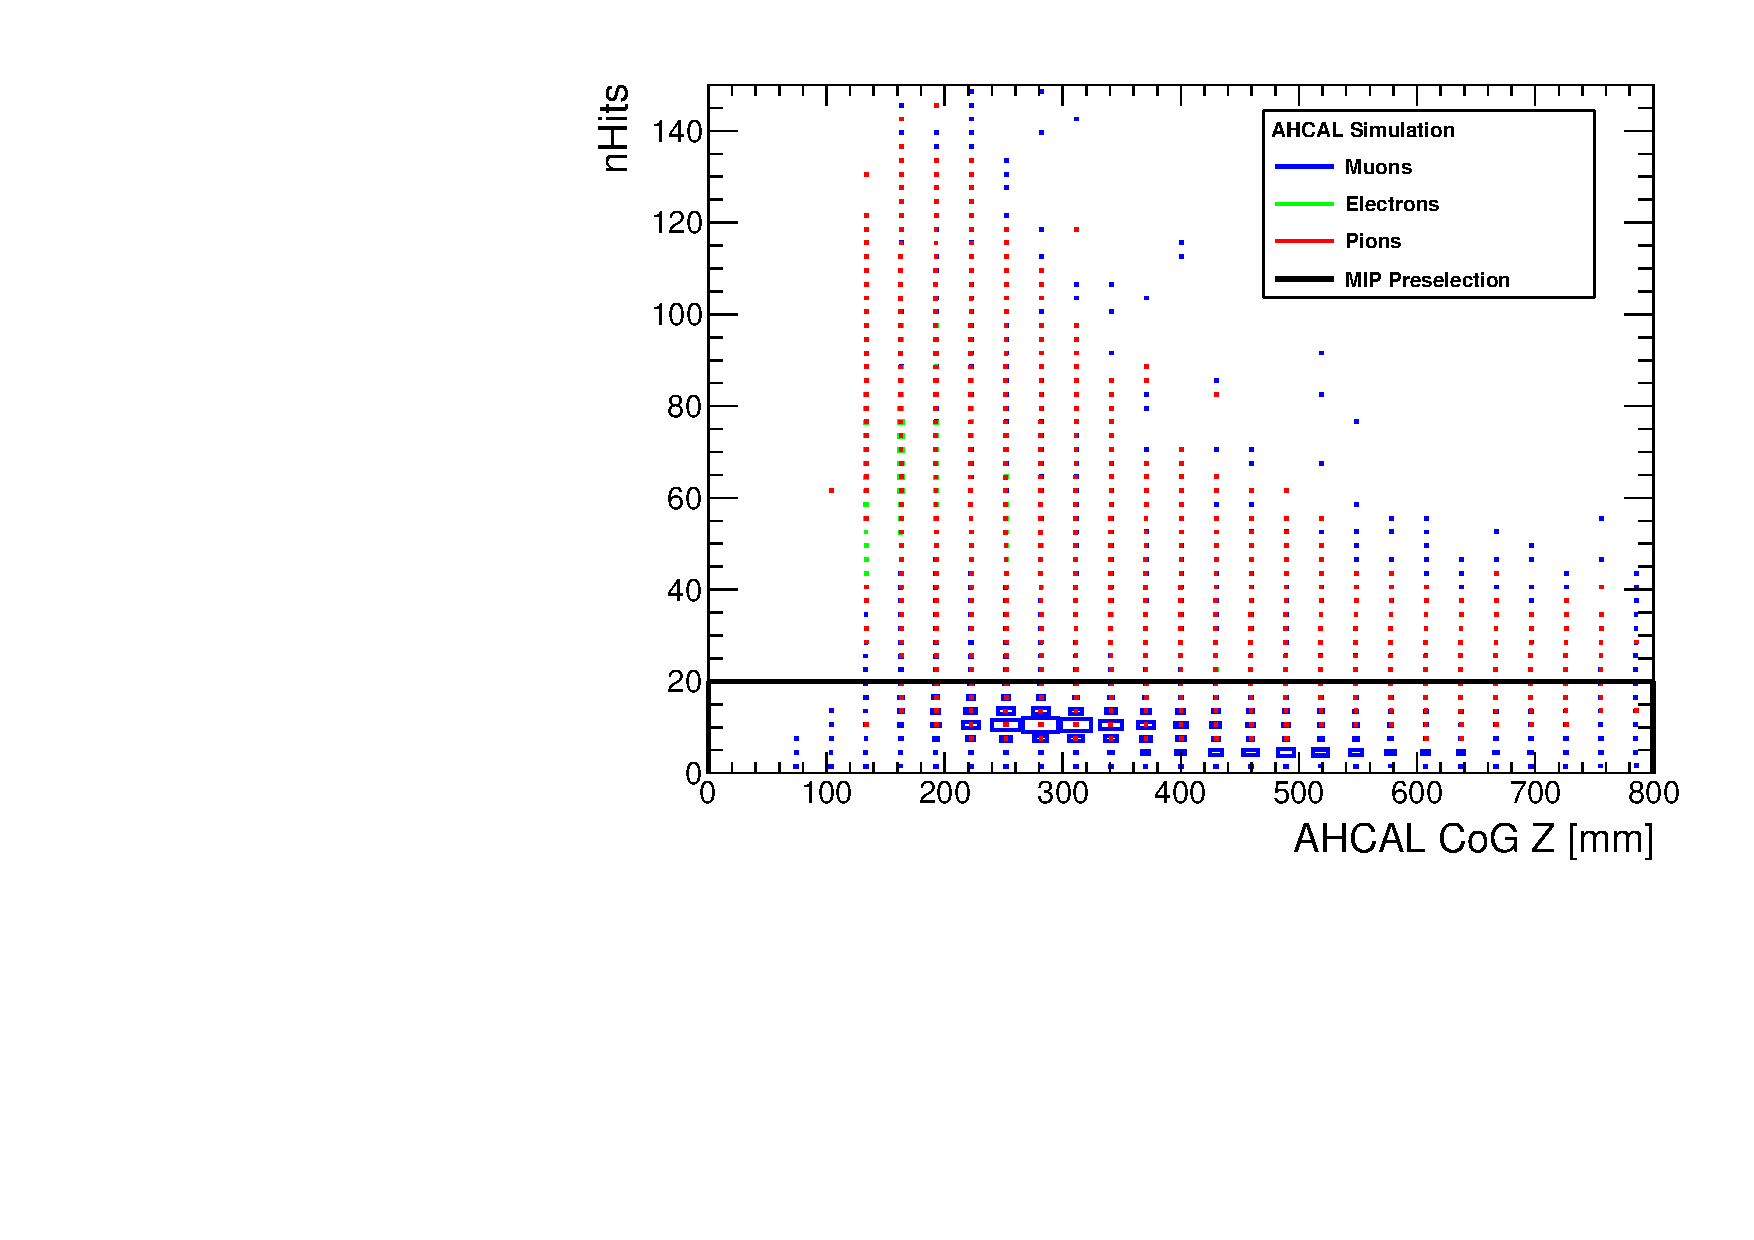
\includegraphics[width=0.5\linewidth]{chap5/fig_AHCAL_timing/Muons/SelectionCut_nHitsCoGZ_Muons}
	\caption{Event distribution in $cog_Z:n_{Hits}$ plane. The black box represents the space-phase covered by the pre-selection.} \label{fig:Muons_CoGZ_nHits}
\end{figure}

\subsection{MIP Selection}
\label{subsec:Muon_sel}

The muon runs were taken first at 50 GeV then another scan at the end of the campaign was performed at 150 GeV. The muon beam was produced by scrapping the halo of a secondary pion beam using collimators. After investigation, muon runs were contaminated by pions showers especially late and passing though the pre-selection due to the small number of active layers in the back of the calorimeter. A simple estimation provided that around 30\% of the events were contaminated.

The muon selection was designed to efficiently select muons and reject late pion showers. For this, a simple MIP track-finder has been developed based on pre-existing work \cite{Hartbrich:2016bbz}. The algorithm selects AHCAL towers of hits in the same $x:y$ plane and rejects towers under a certain number of hits. In order to select muons or punch-through pions, a straight track of at least 7 hits is required in the whole AHCAL without a hard interaction. This also assumes that the calorimeter was perfectly perpendicular to the beam, any angled tracks would be missed. In addition to reject late pion showers, not more than 2 hits are required per layer accounting for some flexibility with noise hits. The distributions of the maximum number of hits in a layer and the number of hits of a track are shown in figures \ref{fig:Muons_Track_nHitsLayer} and \ref{fig:Muons_Track_nHits} for simulated samples of 50 GeV muons, electrons and pions after pre-selection. The track-finder was performed in two steps for the inner part of the detector of $12 \times 12$ tiles and the outer part of the big layers (BL) in order to catch the halo of muons.

The selection efficiency is 72.5\% for muons, 0\% for electrons and 5.6\% for pions. The selection effectively reduces the contamination of late pion showers by over 50\% and the remaining pion efficiency is well compatible with the fraction of pions traversing the AHCAL without hard interaction. A detailed overview of the MIP selection is given in table \ref{table:muon_sel}.

\begin{figure}[htbp!]
	\begin{subfigure}[t]{0.45\textwidth}
		\centering
		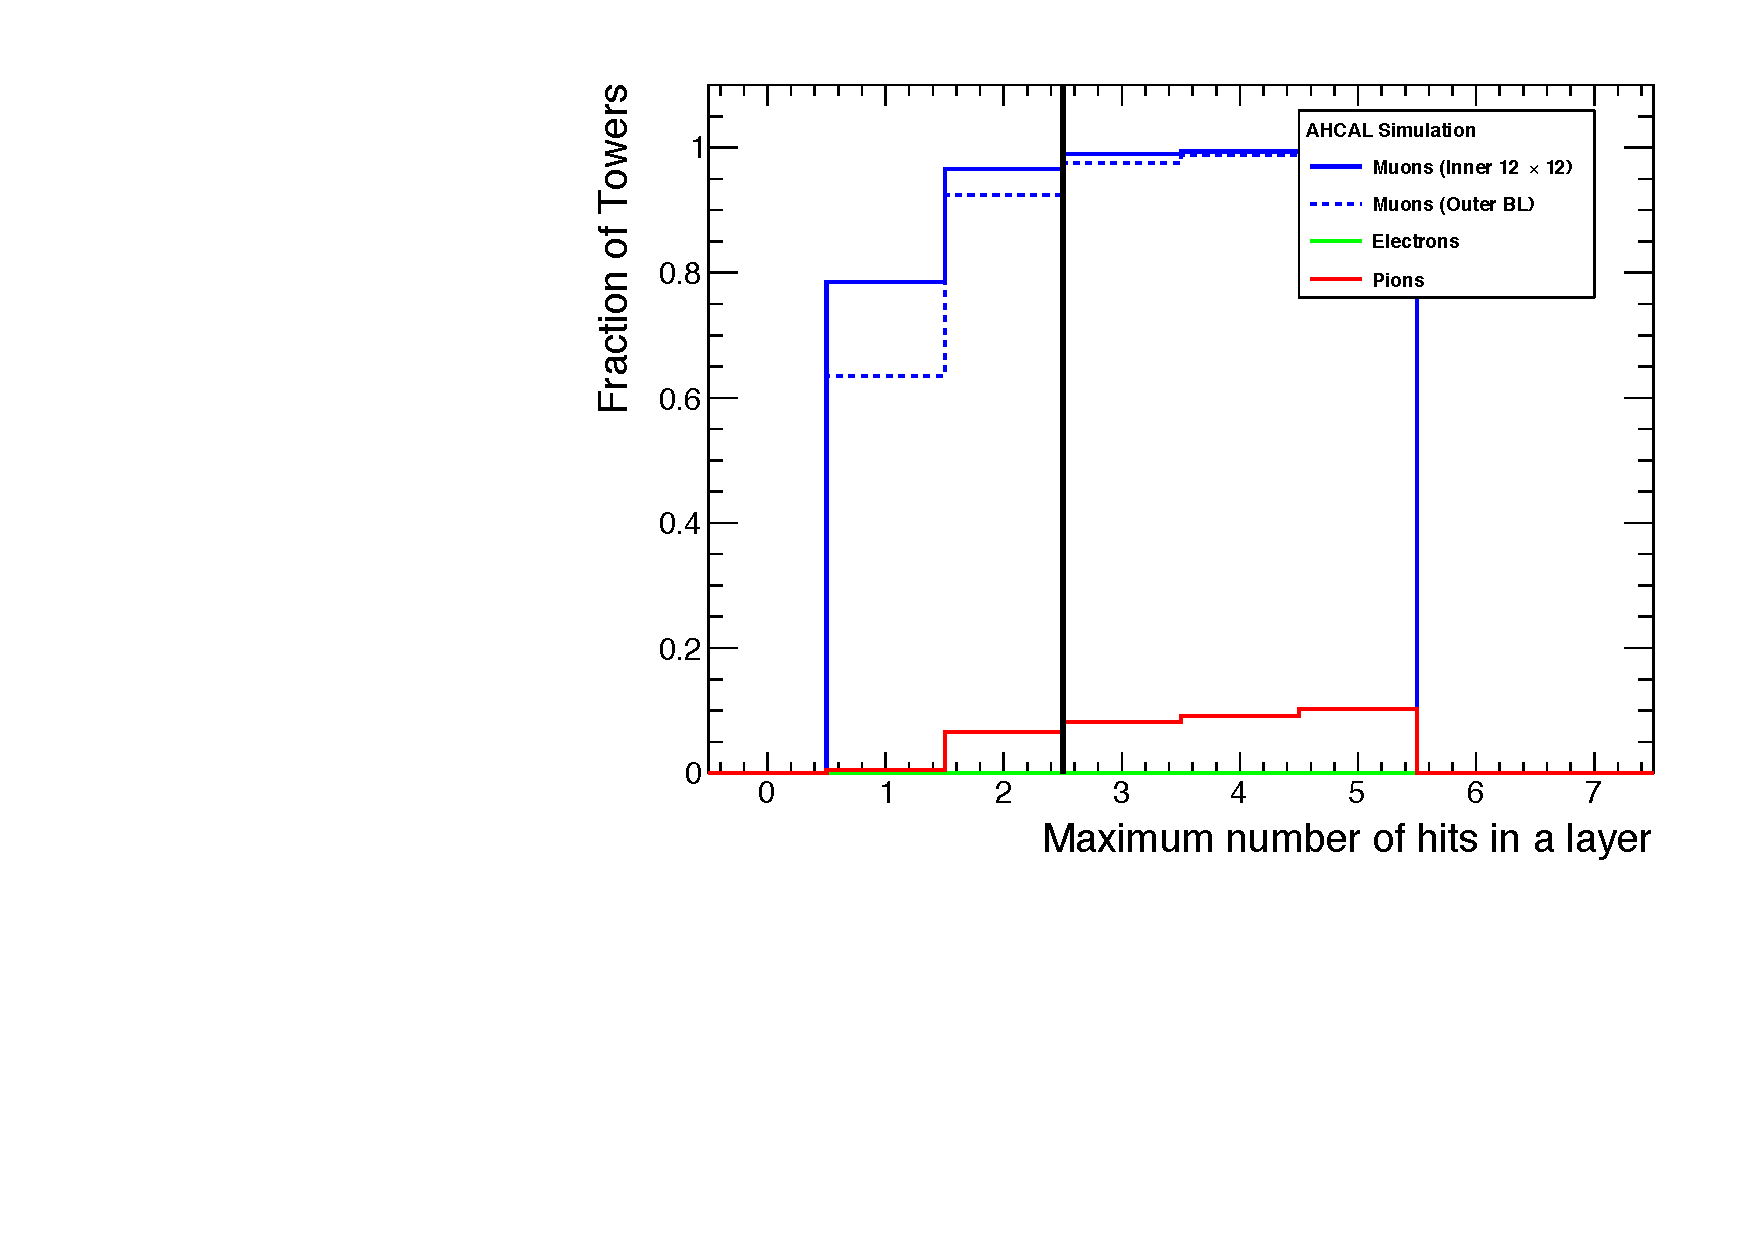
\includegraphics[width=1\linewidth]{chap5/fig_AHCAL_timing/Muons/TrackFinderCut_nHitsLayer_Muons}
		\caption{Maximum number of hits per layer normalized to the number of AHCAL Towers.} \label{fig:Muons_Track_nHitsLayer}
	\end{subfigure}
	\hfill
	\begin{subfigure}[t]{0.45\textwidth}
		\centering
		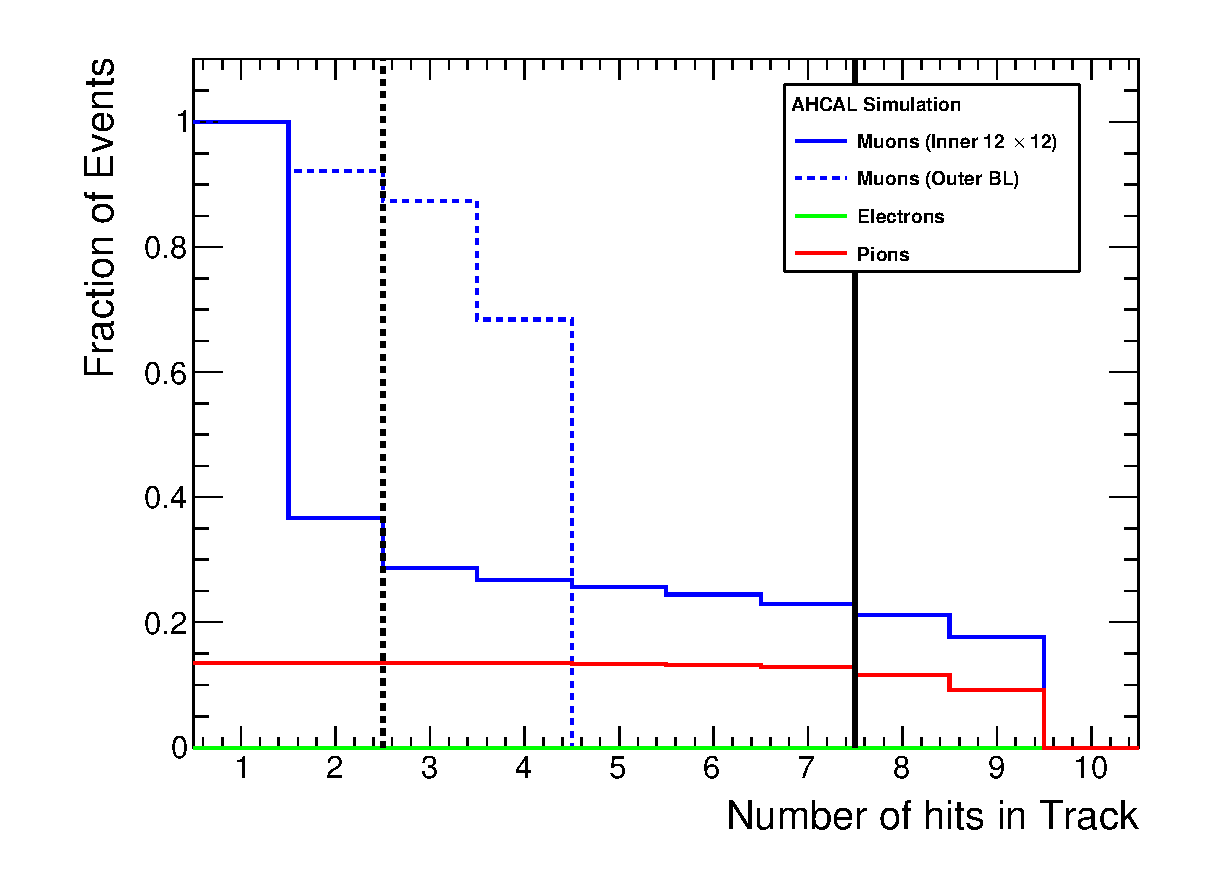
\includegraphics[width=1\linewidth]{chap5/fig_AHCAL_timing/Muons/TrackFinderCut_nHitsTrack_Muons}
		\caption{Number of hits in a track normalized to the number of events.} \label{fig:Muons_Track_nHits}
	\end{subfigure}
	\caption{\subref{fig:Muons_Track_nHitsLayer}) Distribution of the maximum number of hits for simulated muons, electrons and pions at 50 GeV. The black line represents the cut of maximum 2 hits per layer applied for the MIP selection. This cut was done in order to reject late pion showers but avoiding to reject too much of the muons. \subref{fig:Muons_Track_nHits}) Distribution of the number of hits in a track for simulated muons, electrons and pions at 50 GeV. A Tower size of 7 for the inner detector and 2 for the outer big layers was chosen.}
\end{figure}

\subsection{Electron Selection}
\label{subsec:elec_sel}

The electron selection is done to simply extract single electron showers contained in the AHCAL. These events are needed in order to validate the timing behavior in simulation as well as the detector simulation model. For the selection, an \textit{Event Quality} pre-selection is done using the beam instrumentation and layer information. Only events with a Cherenkov tag (only applied on data) are used and as well the energy in the three first layer of the AHCAL ($E_3+E_4+E_5$) must be over 10 MIP. Distributions of the energy in the three first layer of the AHCAL for simulated 10 and 50 GeV muons, electrons and pions can be seen on figures \ref{fig:e10GeV_E3} and \ref{fig:e50GeV_E3}.

In a next step, the electron selection is performed. Due to the number of unusable layers especially the front ECAL layers and the fact that the detector is not fully equipped, an alternative selection needed to be performed to effectively select electrons. As no look into calorimeter linearity and energy resolution is done in this thesis, a cut on the number of hits per event ($n_{Hits}$) versus the center of gravity in z ($CoG_Z < 250 mm$) can be done. This does not induce any bias for a timing analysis, just would only slightly reduce the event statistic.

To ensure a complete containment of the shower and a rejection of possible pion showers, an additional cut on the energy deposited in the last two layers ($(E_{13}+E_{14})/\Sigma E$) is done and must be under 1\% of the energy sum of the event. Distributions of each selection cut are shown in figures \ref{fig:e10GeV_nHitsCoGZ}, \ref{fig:e50GeV_nHitsCoGZ}, \ref{fig:e10GeV_Elast} and \ref{fig:e50GeV_Elast} for simulated 10 GeV and 50 GeV muons, electrons and pions. Due to the restriction on the number of hits per event, the cuts are energy dependent. Additionally to reduce transverse leakage, the shower center of gravity in X and Y needs to be within $-90 mm$ and $90 mm$.

The selection cuts are summed up in table \ref{table:electron_sel} for each energies. The selection efficiency between 10 and 50 GeV are shown in table \ref{table:eff_electron} obtained from simulated samples of muons, electrons and pions with QGSP\_BERT\_HP physics list.

\begin{table}[htb!]
	\centering
	\caption{Electron selection efficiency for between 10 and 50 GeV.}
	\label{table:eff_electron}
	\begin{tabular}{@{} llll @{}}
		\hline
		\textbf{Beam Energy} & \textbf{$\epsilon_{\mu}$} & \textbf{$\epsilon_{e}$} & \textbf{$\epsilon_{\pi}$}\\
		\hline
		10 GeV & <0.1\% & 96\% & 15.9\%\\
		15 GeV & <0.1\% & 95.7\% & 10.1\%\\
		20 GeV & <0.1\% & 95.2\% & 6.3\%\\
		30 GeV & <0.1\% & 93.9\% & 2.3\%\\
		40 GeV & <0.1\% & 92.7\% & 1.2\%\\
		50 GeV & <0.1\% & 91.5\% & 1.1\%\\
		\hline
	\end{tabular}
\end{table}

\begin{figure}[htbp!]
	\begin{subfigure}[t]{0.45\textwidth}
		\centering
		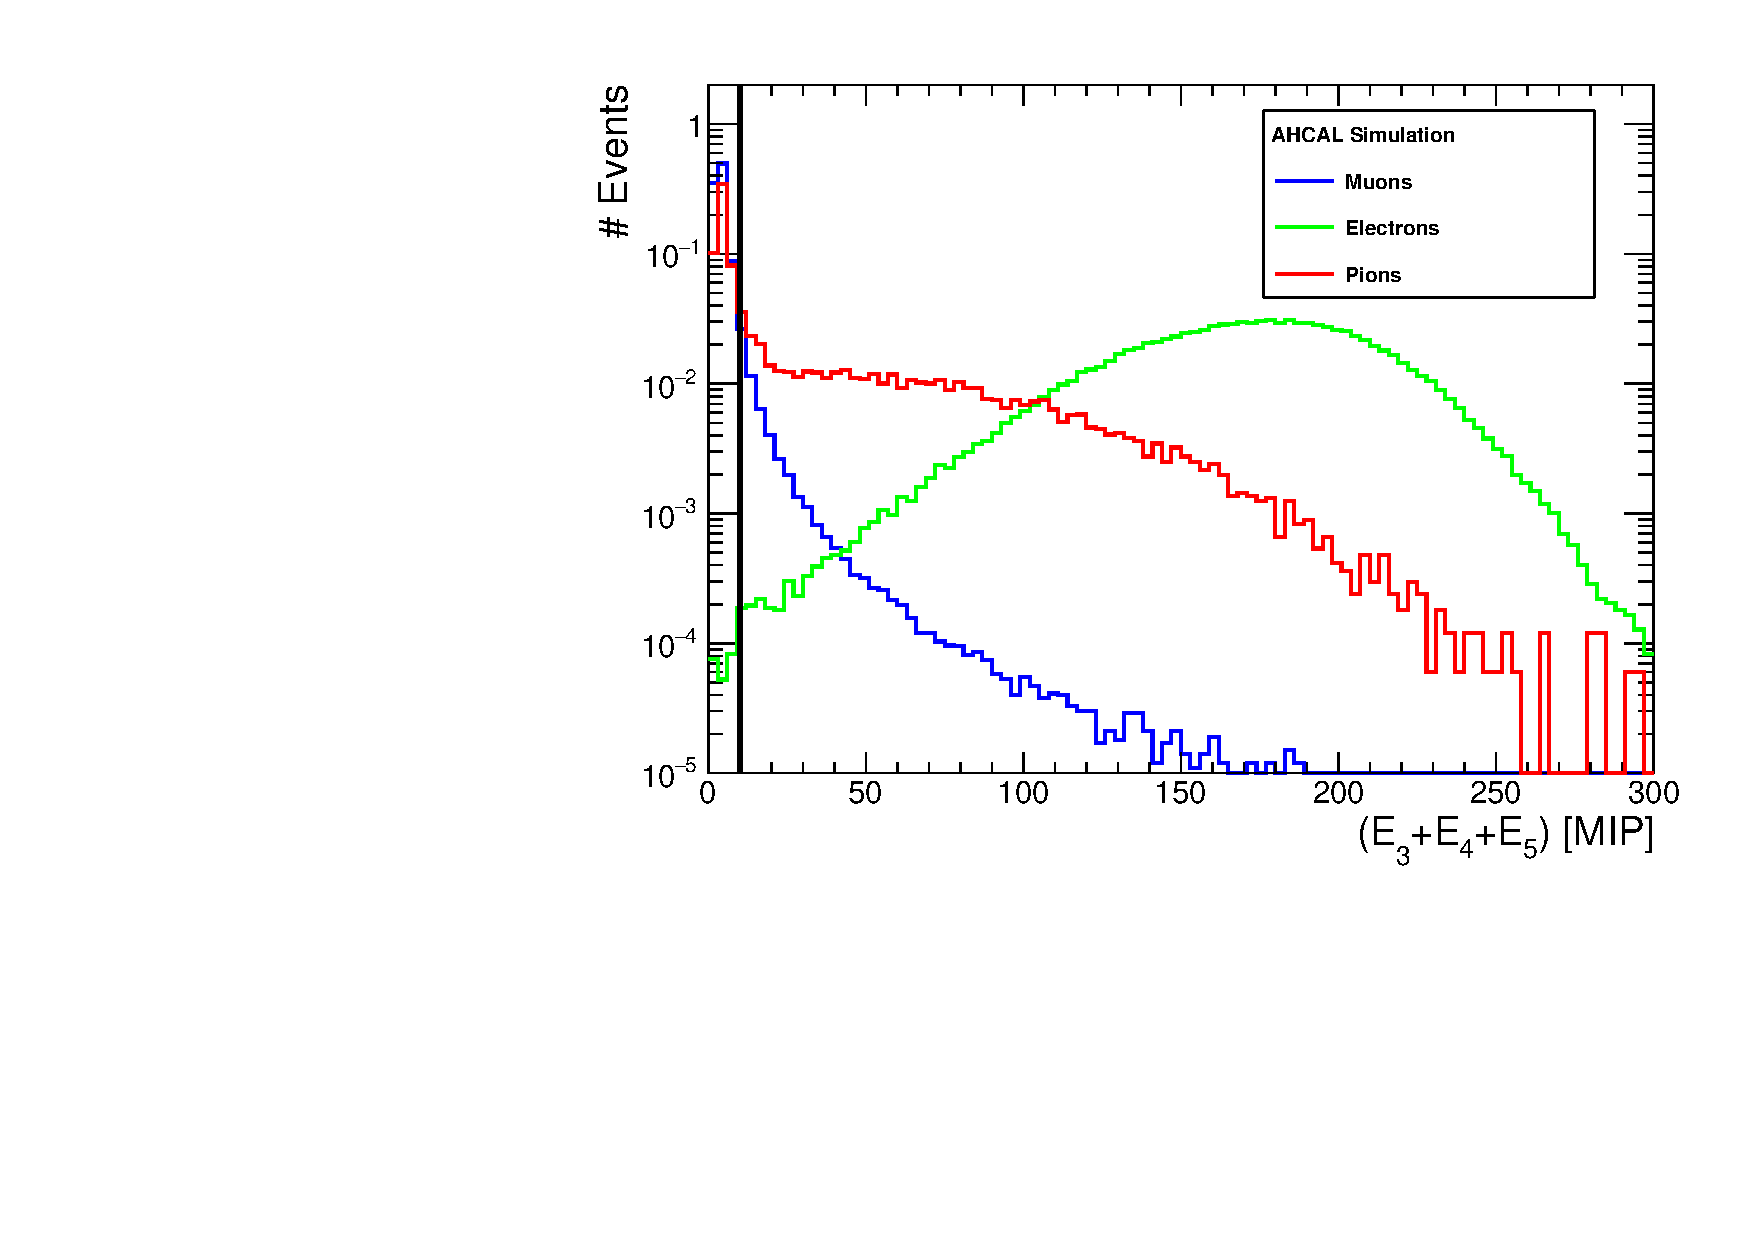
\includegraphics[width=1\linewidth]{chap5/fig_AHCAL_timing/Electrons/SelectionCut_EnergyE3_10GeV}
		\caption{10 GeV.} \label{fig:e10GeV_E3}
	\end{subfigure}
	\hfill
	\begin{subfigure}[t]{0.45\textwidth}
		\centering
		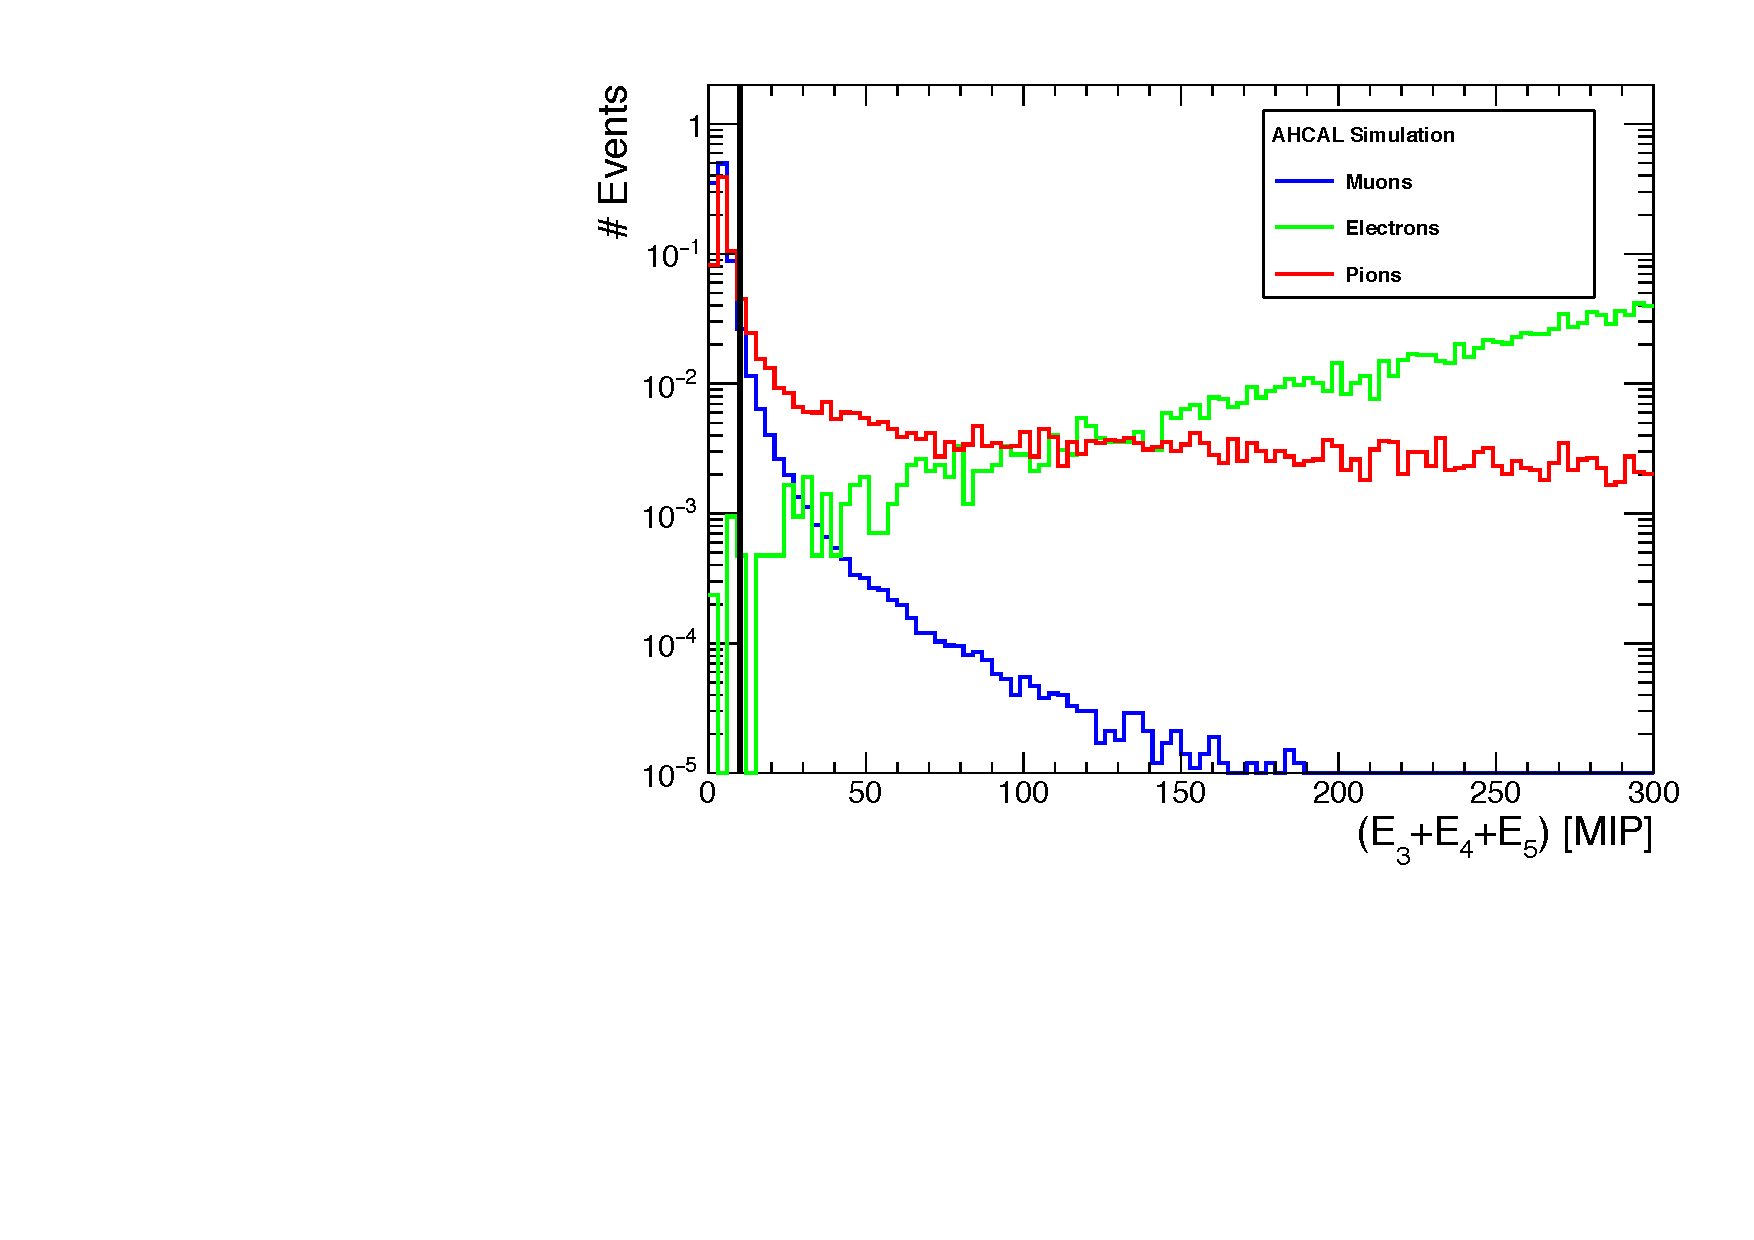
\includegraphics[width=1\linewidth]{chap5/fig_AHCAL_timing/Electrons/SelectionCut_EnergyE3_50GeV}
		\caption{50 GeV.} \label{fig:e50GeV_E3}
	\end{subfigure}
	\hfill
	\begin{subfigure}[t]{0.45\textwidth}
		\centering
		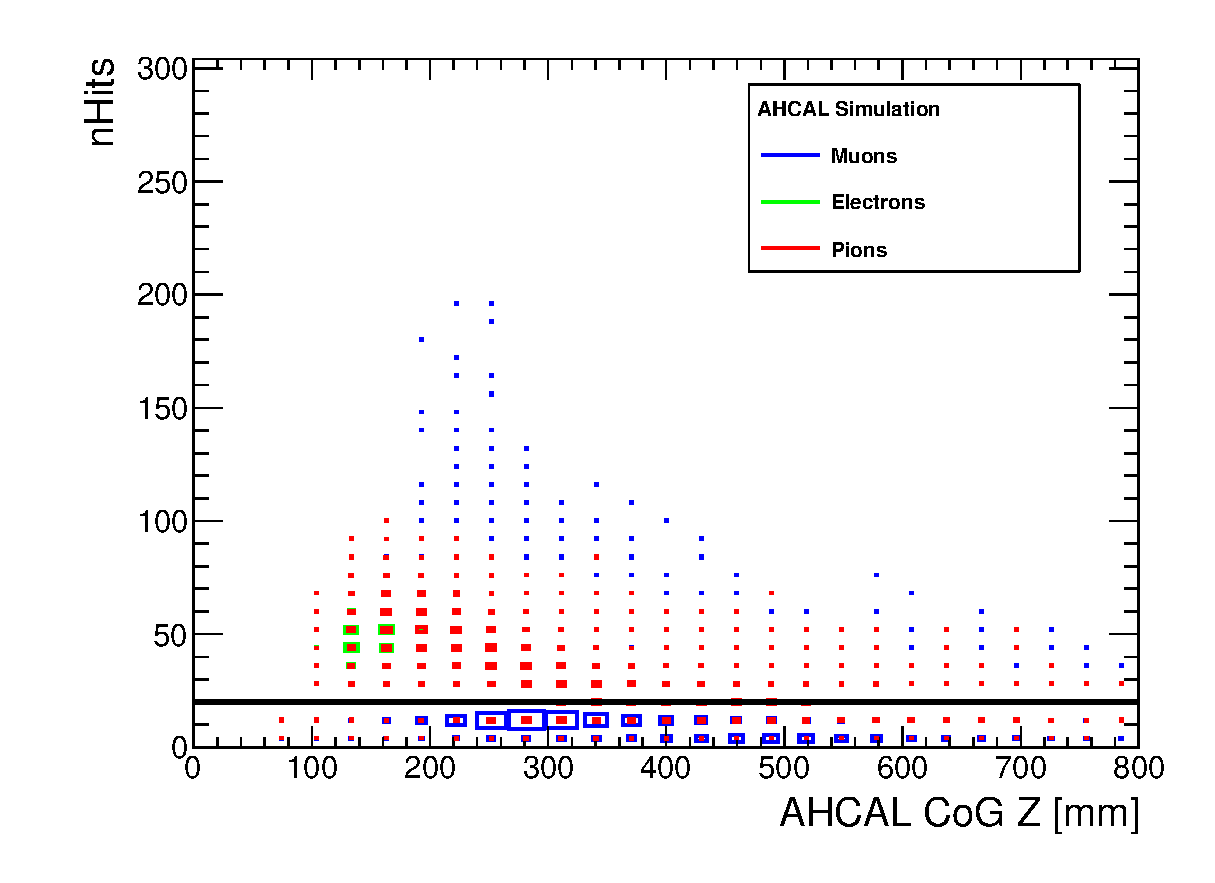
\includegraphics[width=1\linewidth]{chap5/fig_AHCAL_timing/Electrons/SelectionCut_nHitsCoGZ_10GeV}
		\caption{10 GeV.} \label{fig:e10GeV_nHitsCoGZ}
	\end{subfigure}
	\hfill
	\begin{subfigure}[t]{0.45\textwidth}
		\centering
		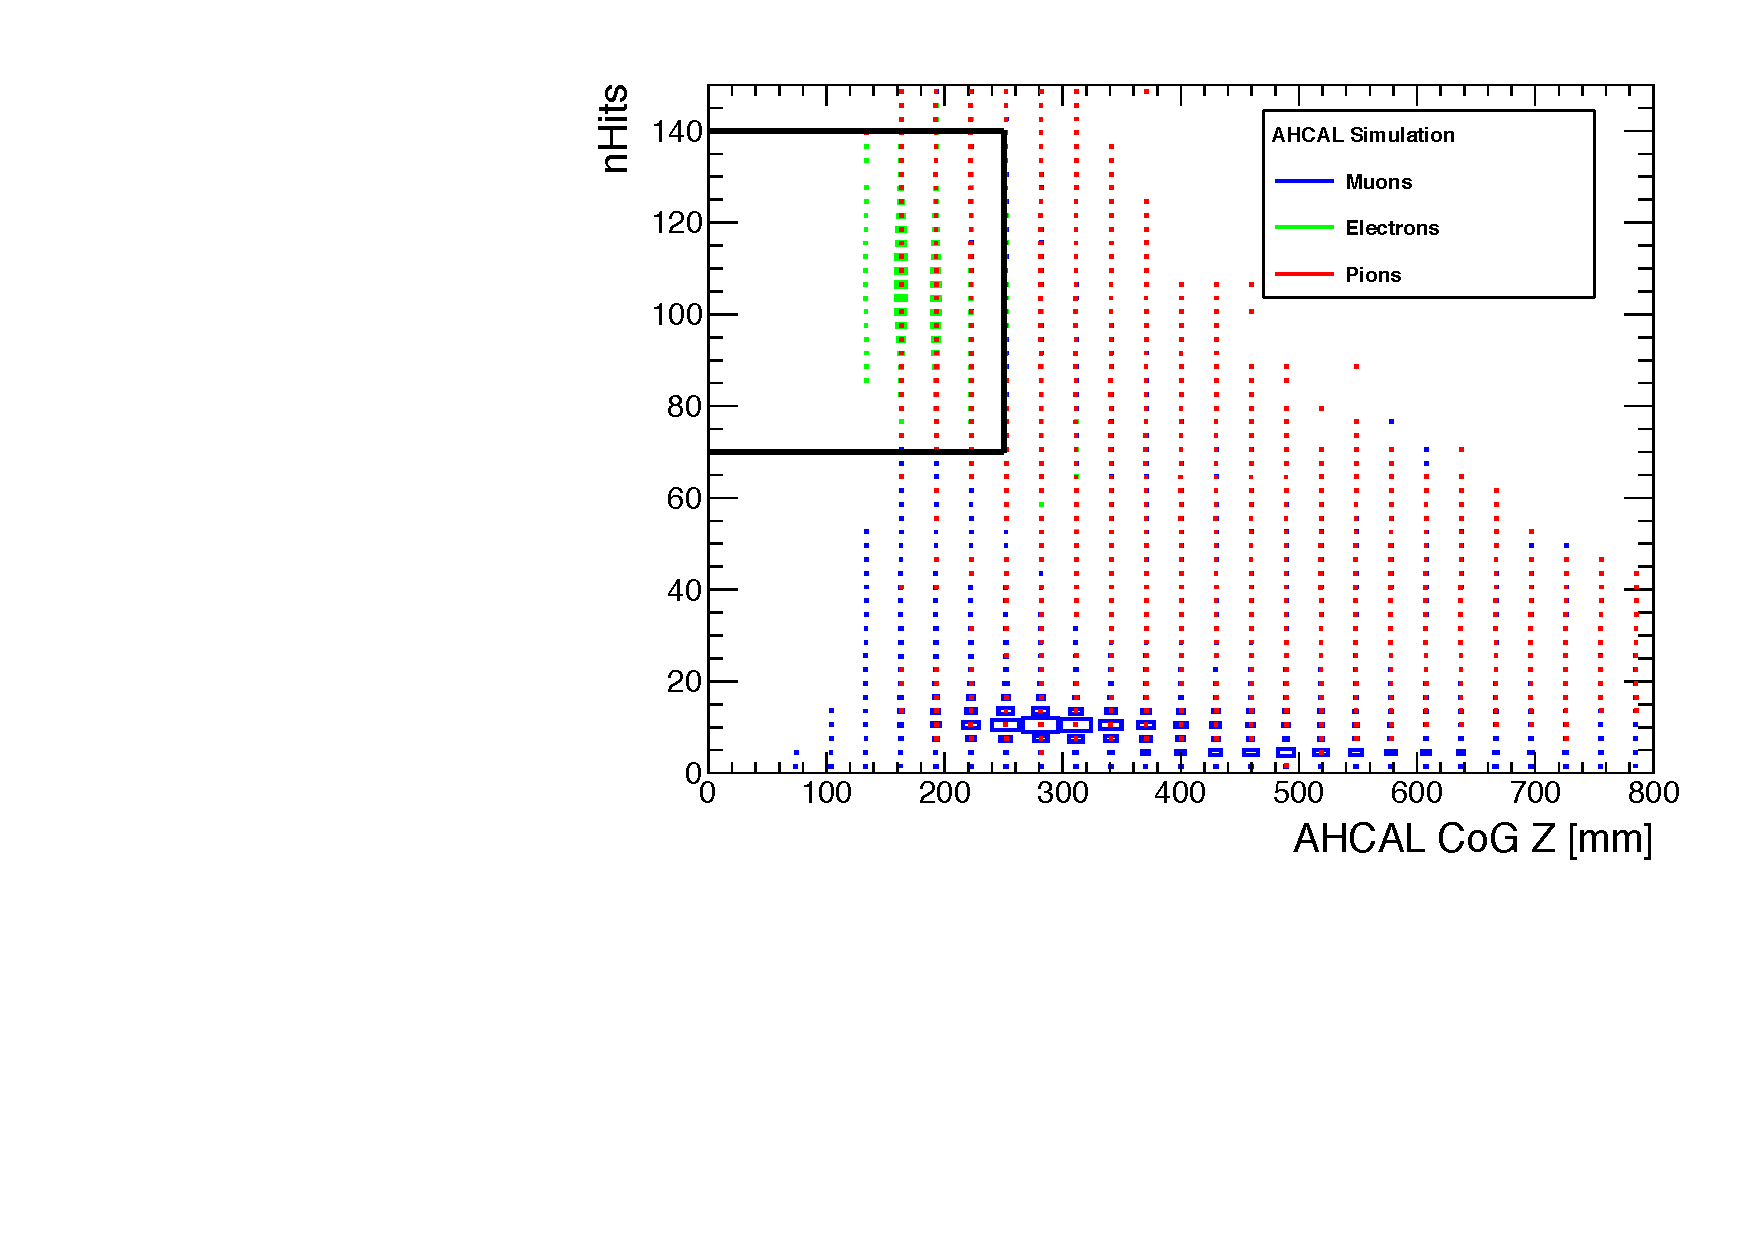
\includegraphics[width=1\linewidth]{chap5/fig_AHCAL_timing/Electrons/SelectionCut_nHitsCoGZ_50GeV}
		\caption{50 GeV.} \label{fig:e50GeV_nHitsCoGZ}
	\end{subfigure}
	\hfill
	\begin{subfigure}[t]{0.45\textwidth}
		\centering
		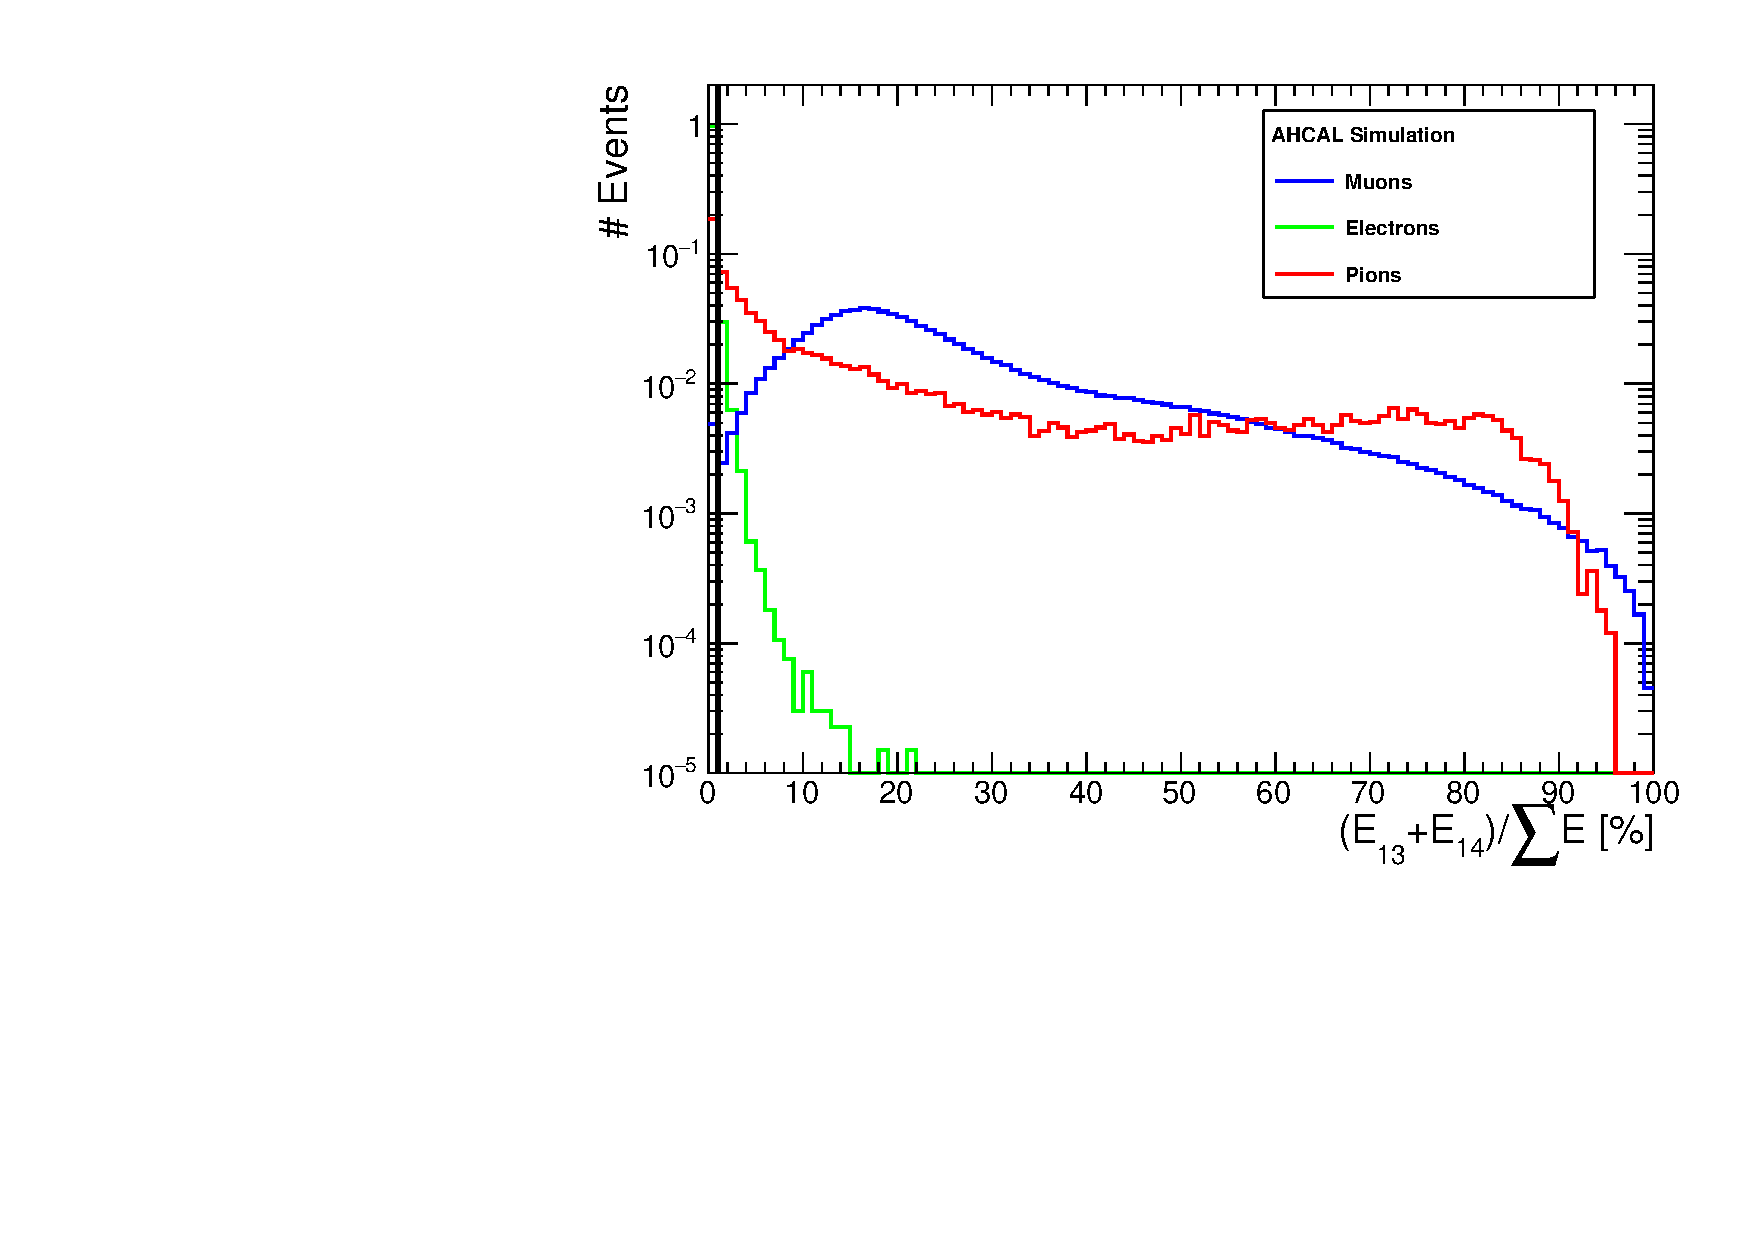
\includegraphics[width=1\linewidth]{chap5/fig_AHCAL_timing/Electrons/SelectionCut_EnergyLastLayers_10GeV}
		\caption{10 GeV.} \label{fig:e10GeV_Elast}
	\end{subfigure}
	\hfill
	\begin{subfigure}[t]{0.45\textwidth}
		\centering
		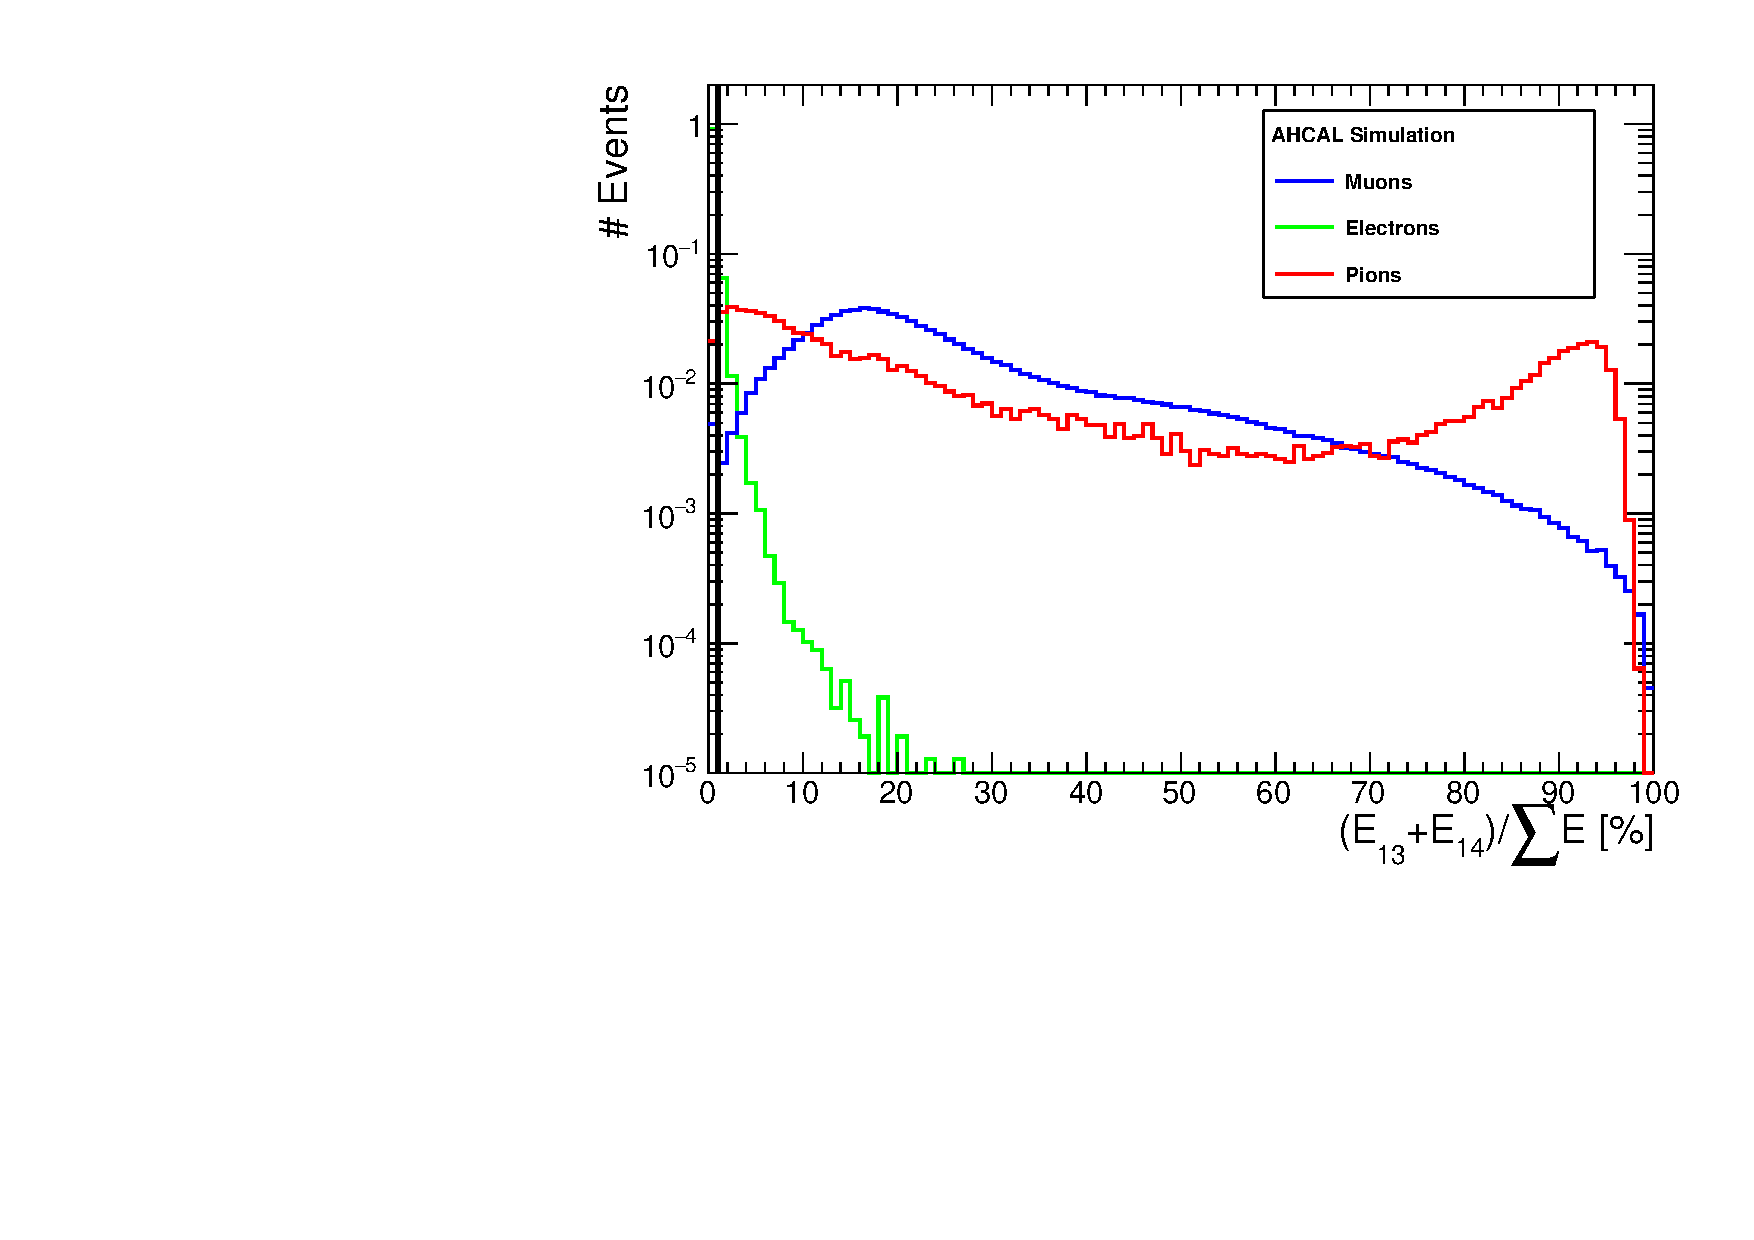
\includegraphics[width=1\linewidth]{chap5/fig_AHCAL_timing/Electrons/SelectionCut_EnergyLastLayers_50GeV}
		\caption{50 GeV.} \label{fig:e50GeV_Elast}
	\end{subfigure}
	\caption{\subref{fig:e10GeV_E3}) . \subref{fig:e50GeV_E3}) . \subref{fig:e10GeV_nHitsCoGZ}) . \subref{fig:e50GeV_nHitsCoGZ}) . \subref{fig:e10GeV_Elast}) . \subref{fig:e50GeV_Elast}) .}
\end{figure}

\subsection{Pion Selection}

A simple selection is performed on pion events. The goal is to reject punch-through pions, muons and possible electron contamination. The selection is similar as the electron selection. An \textit{Event Quality} pre-selection is performed utilizing the Cherenkov information, events with no Cherenkov ON are selected, this is only applied to data. The pion selection is based on the same variables: $cog_Z:n_{Hits}$ plane, $(E_{13}+E_{14})/\Sigma E$ and additionally the number of hits in two first AHCAL layers ($N_3+N_4$). The number of hits required per event needs to be over 20 to reject most muons or punch-through pions without cutting on the center of gravity in z in order not to bias the selection on the start of the pion shower. To ensure that the pion showered, the energy in the last two layers of the AHCAL must be over 1\%. And finally, to mitigate possible particle contamination from electrons, the number of hits in the two first AHCAL layer must be under 5.

Moreover, after a long investigation, multiple particle events were observed in the data. As no beam instrumentation could be utilized for rejecting these events, a simple rejection method based on time clusters was developed. All hits per event are placed and ordered in time in a vector. For each hits after 50 ns, a window of 30 ns is looked after and the number of hits in that window is counted. If the number of hits is over 5, it is counted as a late cluster. The event is rejected if the number of late clusters is over a zero. This method was based on data in order to remove efficiently multi-particle events.

A detailed description of the selection cuts are shown in table \ref{table:pion_sel}.

\begin{table}[htb!]
	\centering
	\caption{Pion selection efficiency between 10 and 90 GeV before multi particle rejection.}
	\label{table:eff_electron}
	\begin{tabular}{@{} llll @{}}
		\hline
		\textbf{Beam Energy} & \textbf{$\epsilon_{\mu}$} & \textbf{$\epsilon_{e}$} & \textbf{$\epsilon_{\pi}$}\\
		\hline
		10 GeV & \% & \% & \%\\
	 	30 GeV & \% & \% & \%\\
		50 GeV & \% & \% & \%\\
		70 GeV & \% & \% & \%\\
		90 GeV & \% & \% & \%\\
		\hline
	\end{tabular}
\end{table}

\section{Timing Calibration}

To perform the timing calibration of the AHCAL, the complete muon dataset is used. The electron dataset is used in a next step to validate the calibration procedure as described in subsection \ref{subsec:validation}. Table \ref{table:mu_elec_runs} summarizes the runs and datasets used. Raw events are considered if the reference signals T$_{12}$,  T$_{13}$ and T$_{14}$ are present in the event. Selected events are counted after the selection on the error of the time reference as explained in \ref{subsection:time_ref}.

\begin{table}[htb!]
	\centering
	\caption{Table with the statistic before and after selection used for timing calibration.}
	\label{table:mu_elec_runs}
	\resizebox{0.9\textwidth}{!}{%
	\begin{tabular}{@{} llllll @{}}
		\hline
		Runs & Energy & Particle Type & Events (Raw) & Events (sel.) & $\frac{\text{N$_{sel.}$}}{\text{N$_{raw}$}}$ \\
		\hline
		24016-24663 & 50-150 GeV & $\mu^-$ & 1851536 & 836796 & 45.2\% \\
		24528-24577 & 10 GeV & $e^-$ & 268275 & 216656 & 80.8\% \\
		24510-24520 & 15 GeV & $e^-$ & 108092 & 90395 & 83.6\% \\
		24486-24504 & 20 GeV & $e^-$ & 130232 & 110161 & 84.6\% \\
		24460-24470 & 30 GeV & $e^-$ & 82202 & 69692 & 84.8\% \\
		24427-24435 & 40 GeV & $e^-$ & 65901 & 55660 & 84.5\% \\
		24405-24419 & 50 GeV & $e^-$ & 123422 & 104030 & 84.3\% \\
		\hline
	\end{tabular}
	}
\end{table}

\subsection{Slope calibration}
\label{subsec:slope_calib}

The data analysis is performed in several steps. The first step is the calibration of the time provided by the SPIROC2B chip. To reconstruct the time of the first hit (only a single hit per channel is registered during a bunch-crossing) in a channel, the TDC value measured needs to be converted into nanoseconds. The value is converted using the following equations:

\begin{equation} \label{eq:slope}
	\text{slope}_{chip, BXID} \: \text{[ns/TDC]} = \frac{3920 \: \text{ns}}{\text{Max}_{chip, BXID} - \text{Pedestal}_{chip, BXID}}
\end{equation}
\begin{equation} \label{eq:time_chn}
	\text{T}_{chn} \: \text{[ns]} = \text{slope}_{chip, BXID} \times (\text{TDC} - \text{Pedestal}_{mem=1} )
\end{equation}

The determination of the parameter $\text{slope}_{chip, BXID}$ is assuming that the TDC ramp is linear. The parameters Max$_{chip, BXID}$ and Pedestal$_{chip, BXID}$ in eq.\ref{eq:slope} are extracted from the TDC spectrum from a specific chip and BXID using only the first memory cell as illustrated in figure \ref{fig:TDC_Spectrum}. At the same time, the parameter Pedestal$_{mem=1}$ in eq.\ref{eq:time_chn} is extracted from the spectrum for each channel and the first memory cell of a chip without taking into account the BXID of the ramp as the difference between both pedestal can be corrected for at a later stage. This is accounting for a total of 208 slopes and 3744 pedestals to be extracted for the testbeam setup.

\begin{figure}[htbp!]
	\begin{subfigure}[t]{0.45\textwidth}
		\centering
		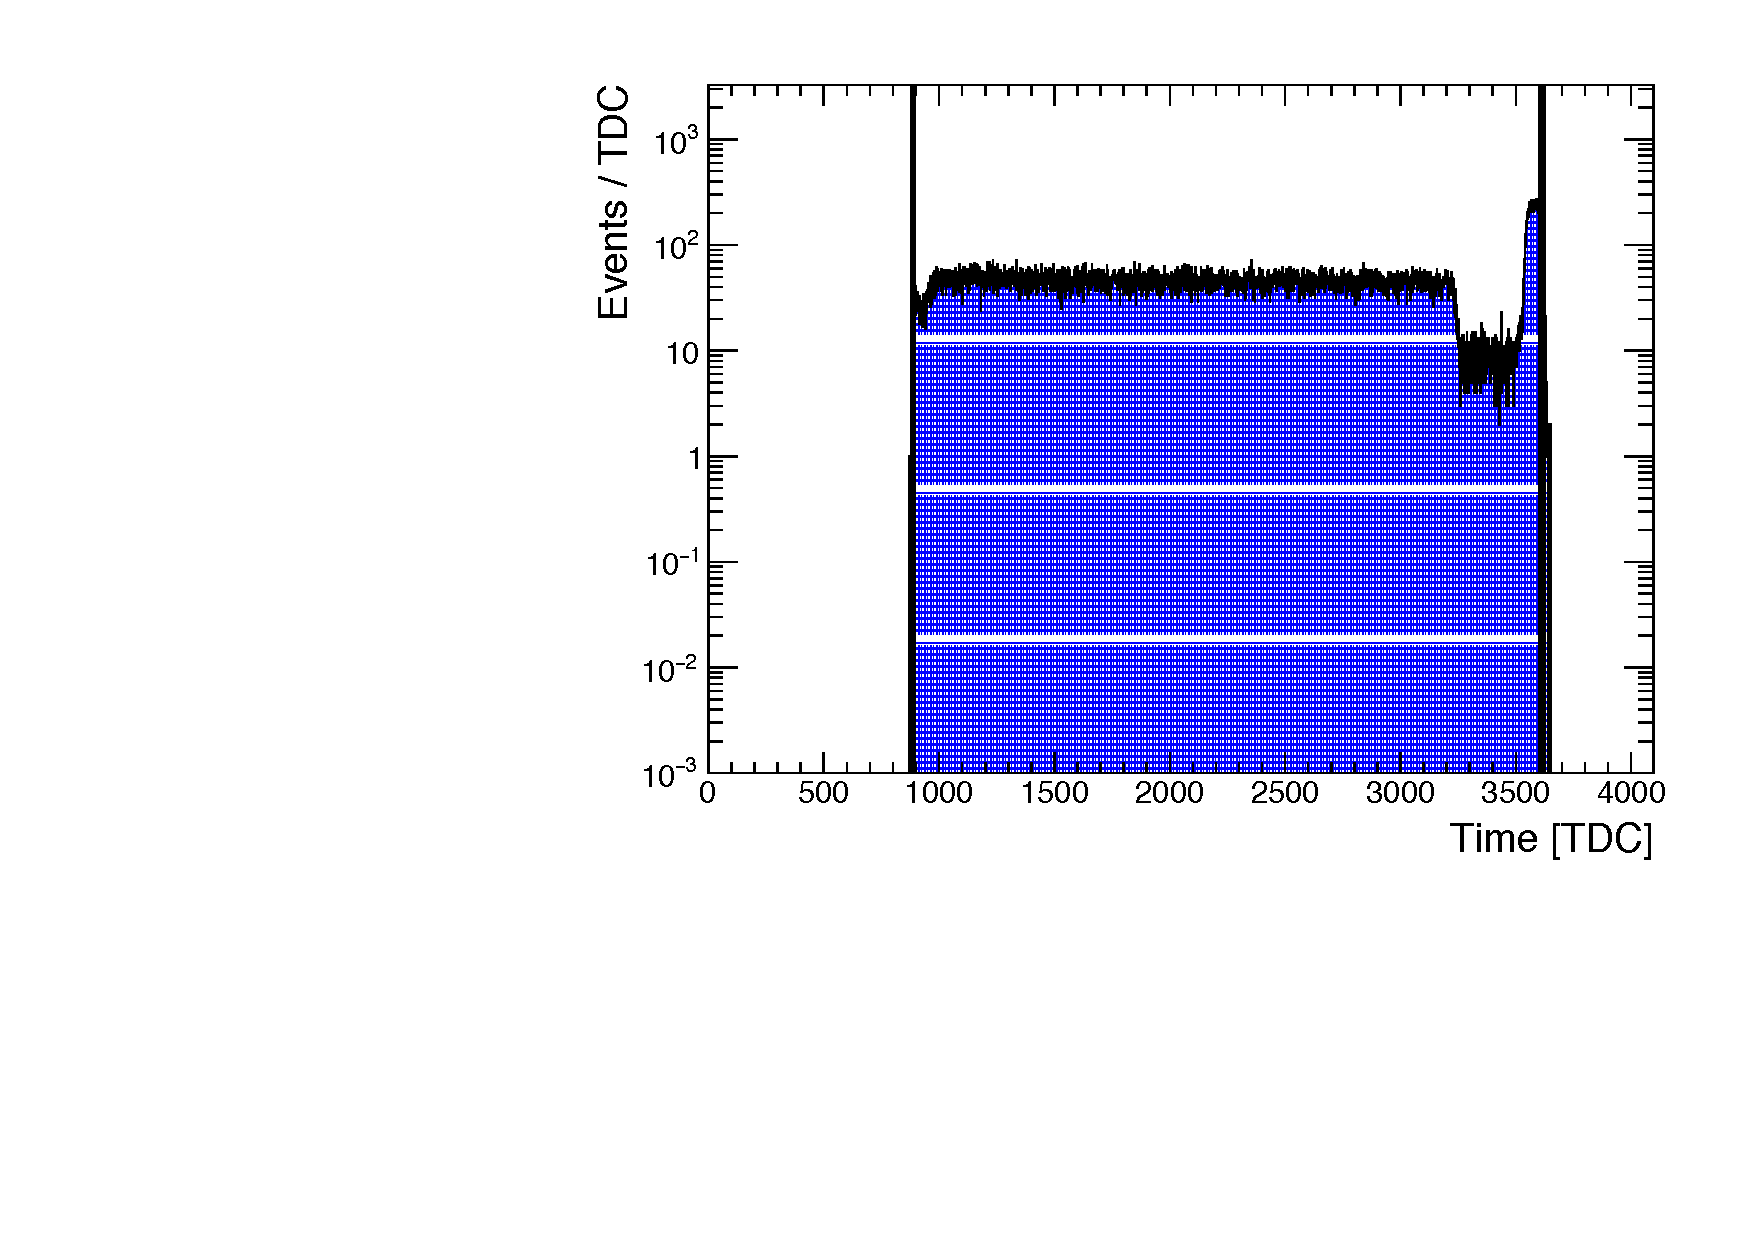
\includegraphics[width=1\linewidth]{chap5/fig_AHCAL_timing/Muons/ExampleTDCSpectra}
		\caption{TDC Spectrum of a typical chip.} \label{fig:TDC_Spectrum}
	\end{subfigure}
	\hfill
	\begin{subfigure}[t]{0.45\textwidth}
		\centering
		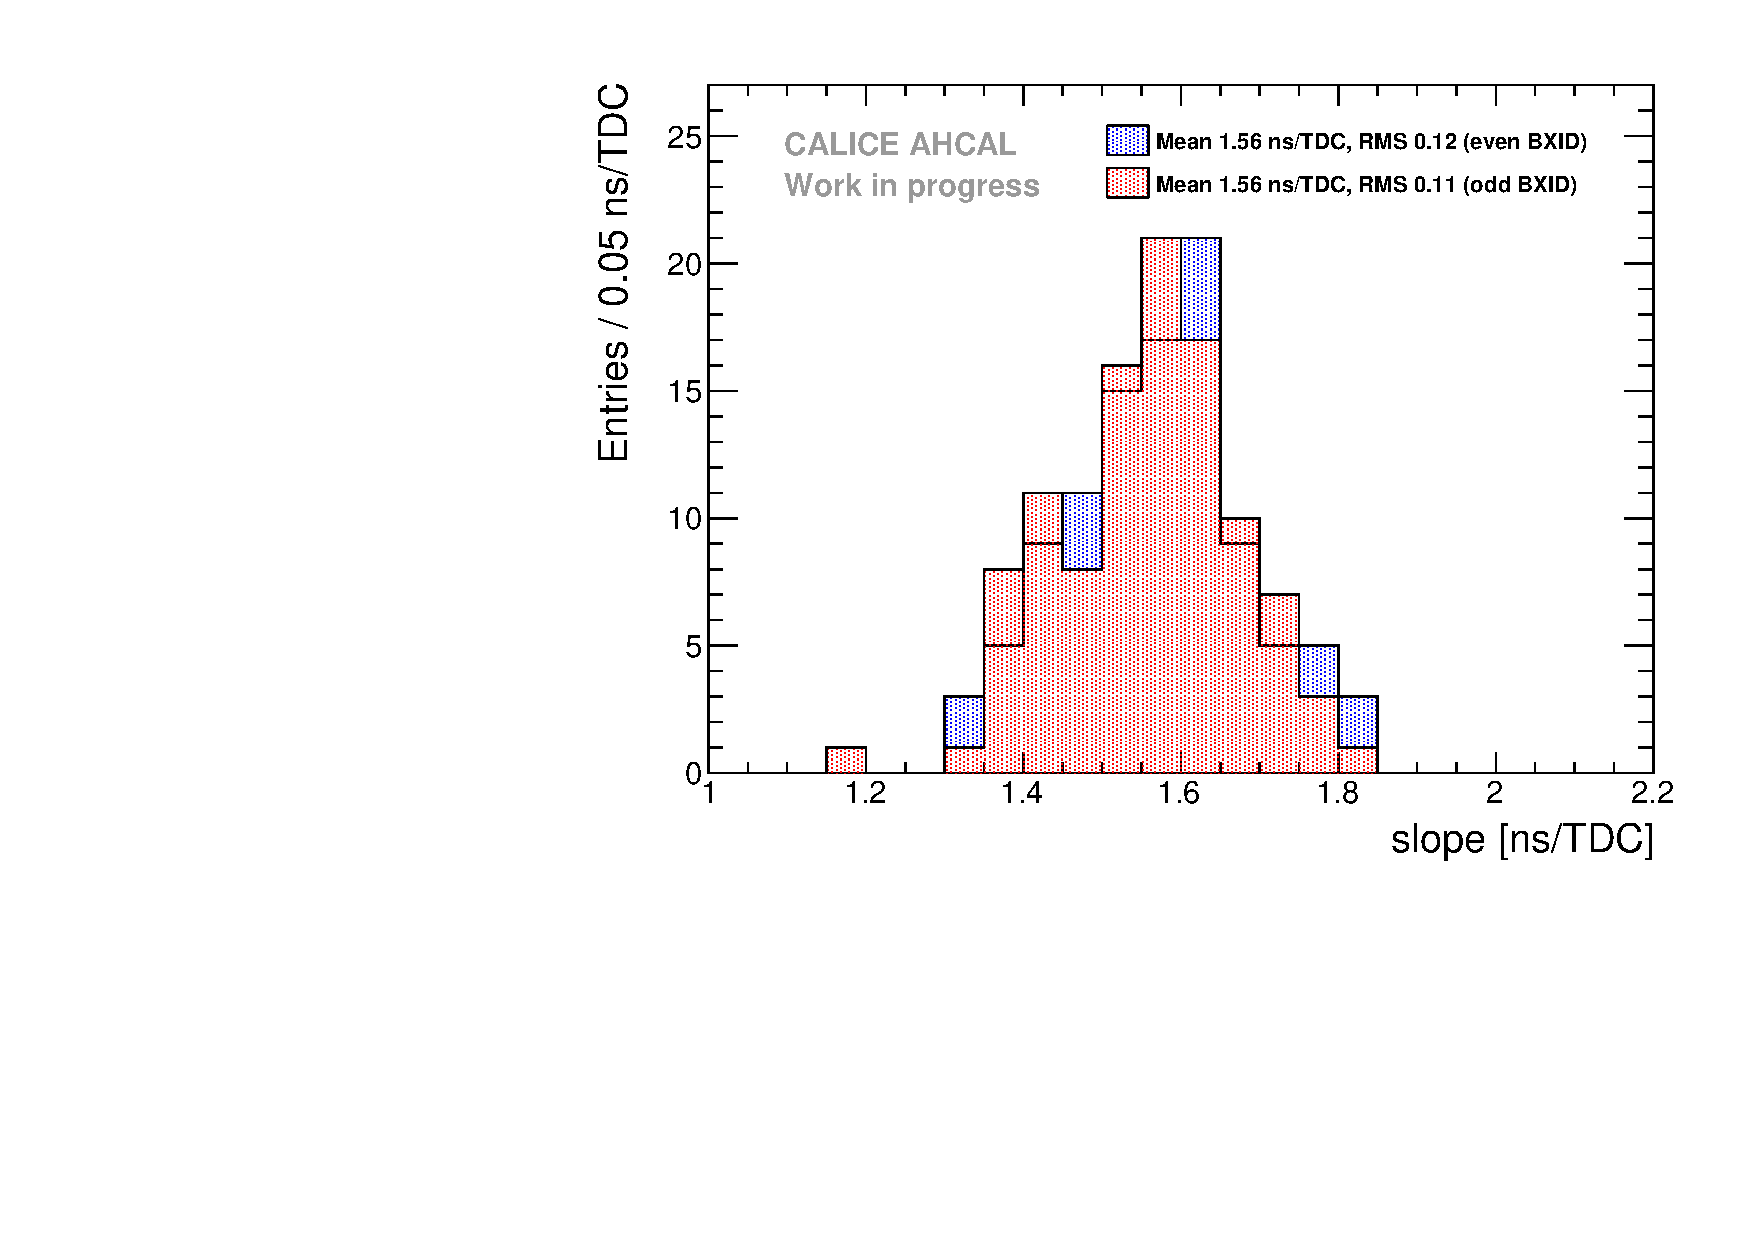
\includegraphics[width=1\linewidth]{chap5/fig_AHCAL_timing/Muons/SlopesTDC}
		\caption{Distribution of the fitted slopes for even and odd bunch-crossing IDs.} \label{fig:slope_time}
	\end{subfigure}
	\caption{\subref{fig:TDC_Spectrum}) The red rectangle are the fitted Max and Pedestal parameters for this chip. The yellow bands represents estimation of the error made on the extraction of the parameters by a variation of 1 RMS of the threshold $\mu$. The parameters extracted are slope = 1.56 $\pm$ 0.01, Pedestal = 816 $\pm$ 9 and Maximum = 3336 $\pm$ 8. \subref{fig:slope_time}) T$\mu_{odd}$ = 1.564 ns/TDC, RMS$_{odd}$ = 0.121, $\mu_{even}$ = 1.556 ns/TDC, RMS$_{even}$ = 0.113.}
\end{figure}

The technique of extraction is based on an edge detection method. For each chip and BXID, an histogram is filled with the y value of each bin then the mean of this histogram is defined as a threshold $\mu$. The parameter Pedestal$_{chip, BXID}$ is extracted as the first bin above 30\% of $\mu$. For the parameter Max$_{chip, BXID}$, it is extracted by taking 50\% of the maximum bin of the original histogram.The maximum seems not to be exactly at the last bin of the spectrum, this is due to the technique that needed to be robust against strange spectra. An estimation of the errors made on the pedestal and maximum is done by looking at the maximum difference between 1 RMS of $\mu$ and 33\% of the maximum bin to the extracted value. More details about the estimations of the calibration errors is described in the appendix \ref{appendix:calib_error}. The extracted values for the slopes are in the expected range of 1.6 ns per TDC bin due to the limited dynamic range provided by the chip (around 2500 bins for 4 $\mu$s) which is in aggreement with figure \ref{fig:slope_time}.

\subsection{Determination of the time of first hit}

\subsubsection{Time reference}
\label{subsection:time_ref}
To reconstruct the time of the first hit in a channel, the measured time of a hit needs to be compared to the time of the reference trigger. The trigger signals described in subsection \ref{subsec:trigger} are calibrated using the same method as explained above. After time calibration of the hit, events are selected by requiring that T$_{12}$, T$_{13}$ and T$_{14}$ are present in the event in a certain amplitude range to reject noise hits from theses channels. In addition, as these channels receive exactly the same signal from the NIM-logic at the same time, a quadratic correction is applied to ensure that they match in time. The correction is performed by correcting the time of T$_{12}$ and T$_{13}$ compared to the time of T$_{14}$. The figure \ref{fig:T0_Correction} shows that the correction reduces the spread of the trigger channels w.r.t to each other. The resulting resolution for the reference trigger signal is around 4-5 ns, this resolution from the electronics contributes to the final timing resolution obtained.

\begin{figure}[htbp!]
	\centering
	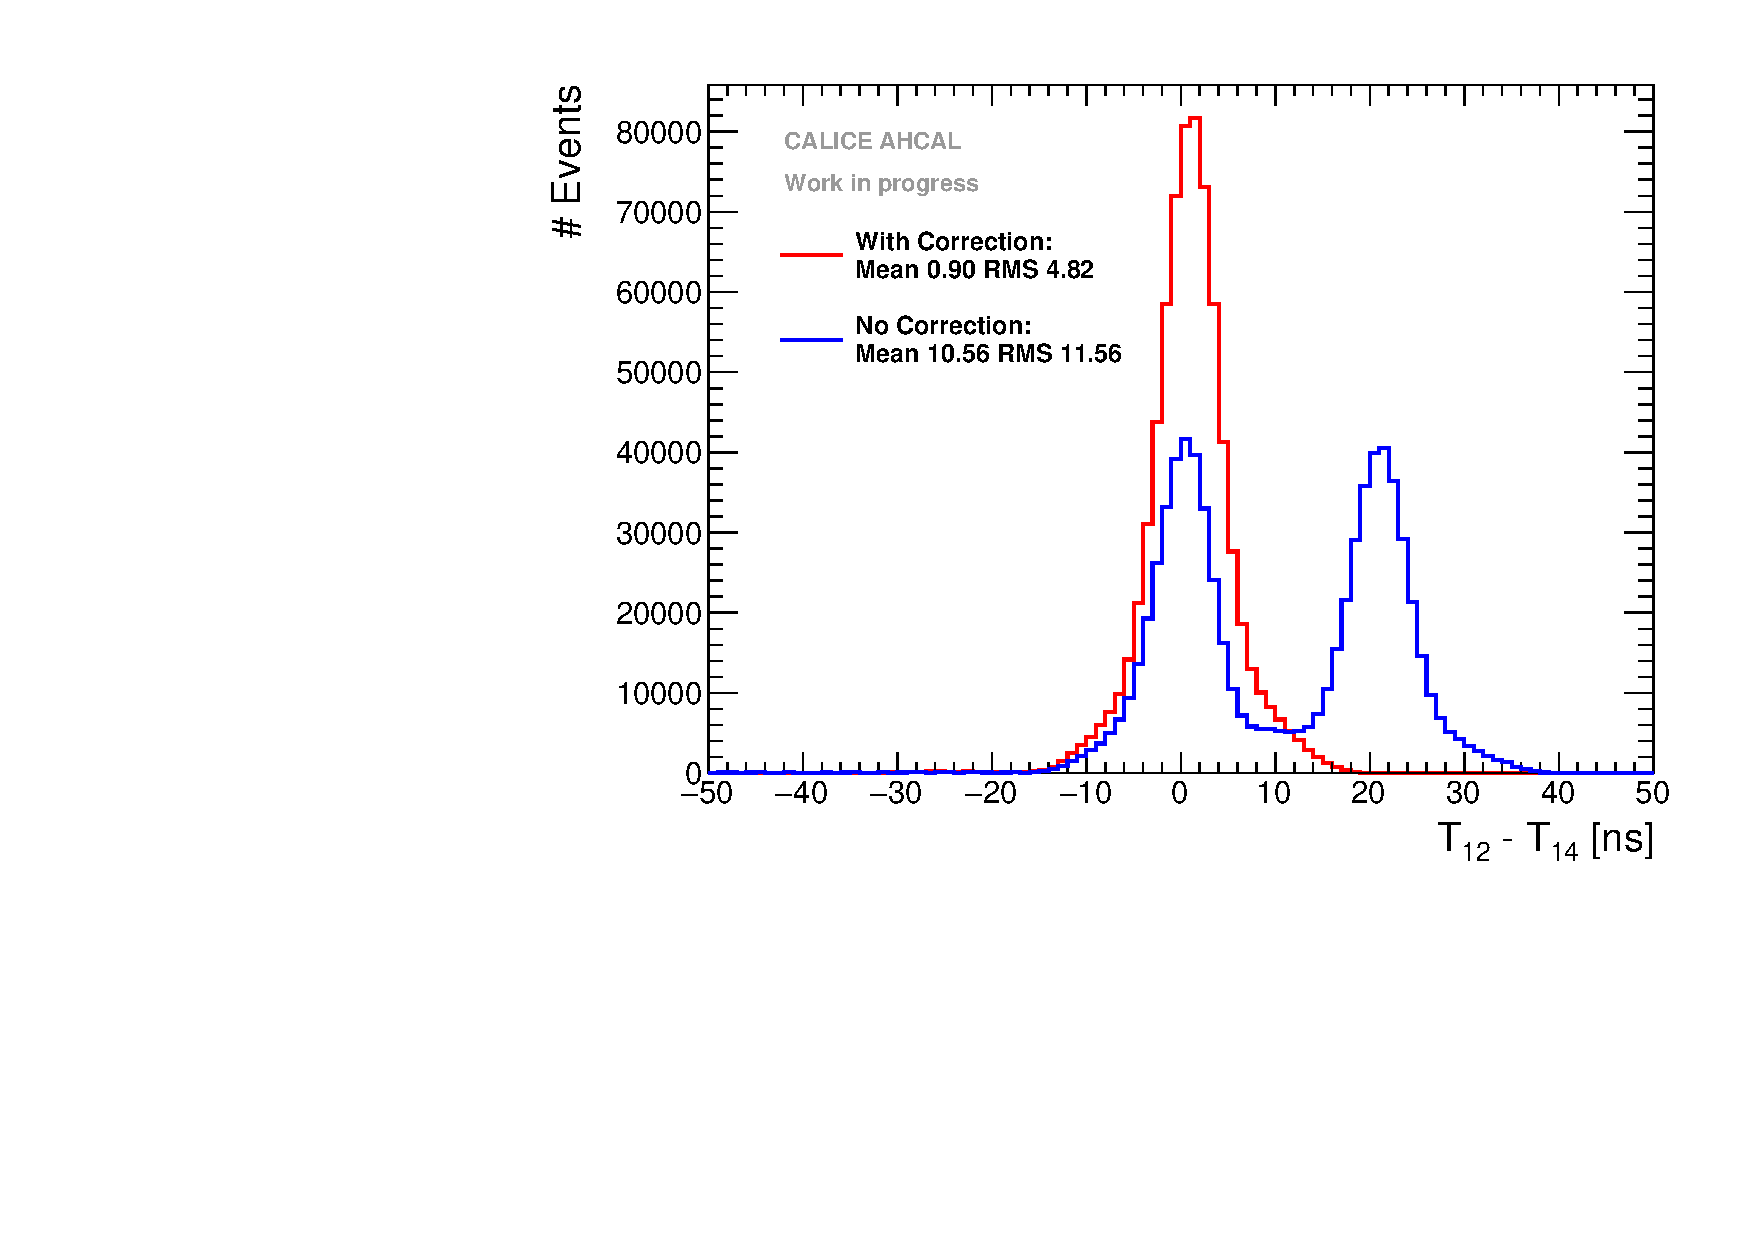
\includegraphics[width=1\textwidth]{chap5/fig_AHCAL_timing/T0s/T0_Resolution_5.pdf}
	\caption{Time difference between the trigger channels before and after correction for T$_{12}$ and T$_{14}$. The histogram in blue shows the difference between the channels before correction, the histogram in red shows the difference after correction. $\mu$ = 10.6 ns, RMS = 11.6 ns, $\mu_{corrected}$ = 0.9 ns, RMS$_{corrected}$ = 4.8 ns}
	\label{fig:T0_Correction}
\end{figure}

In a next step, to reduce the uncertainty made on the time of the trigger, the time reference $T_{ref}$ is calculated using the mean of T$_{12}$, T$_{13}$ and T$_{14}$ and its associated error $\sigma_{ref}$ as shown in eq. \ref{eq:tref} \& \ref{eq:tref_err}. A cut of 4 ns is performed on $\sigma_{ref}$ to reject events with a too large error on the time of the trigger.

\begin{equation} \label{eq:tref}
	\text{T}_{ref} = \frac{\text{T}_{12} + \text{T}_{13} + \text{T}_{14}}{3}
\end{equation}
\begin{equation} \label{eq:tref_err}
	\sigma_{ref}^2 = \frac{ (\text{T}_{12} - \text{T}_{ref})^2 + (\text{T}_{13} - \text{T}_{ref})^2  + (\text{T}_{14} - \text{T}_{ref})^2 }{6}
\end{equation}

Since the absolute time between the passage of a muon and the trigger of a channel is not known due to cabling and the trigger electronics, the time offset relative to the trigger is determined from data. Muons are quasi-instantaneous particles thus the time of the first hit distribution for each channel, memory cells and BXID has to be shifted to \textit{t=0}. This shifting procedure takes into account the delay time of the trigger due to cabling and the NIM-logic as well as mis-calibrations in pedestals. Only memory-cells containing more than 100 events are considered. This offset is determined by iteration requiring at least 4 prompt hits i.e hits in the range from -20 to 20 ns of the event. In this way, 18338 individual offsets are extracted from data. A distribution of the extracted offsets using muon data can be seen in figure \ref{fig:offset_trigger_distribution}. The figure \ref{fig:BXID_offset} shows that individual offsets have to be extracted for each BXID as the correlation is chip-dependent and not the same for odd and even BXIDs.

\begin{figure}[htbp!]
	\begin{subfigure}[t]{0.45\textwidth}
		\centering
		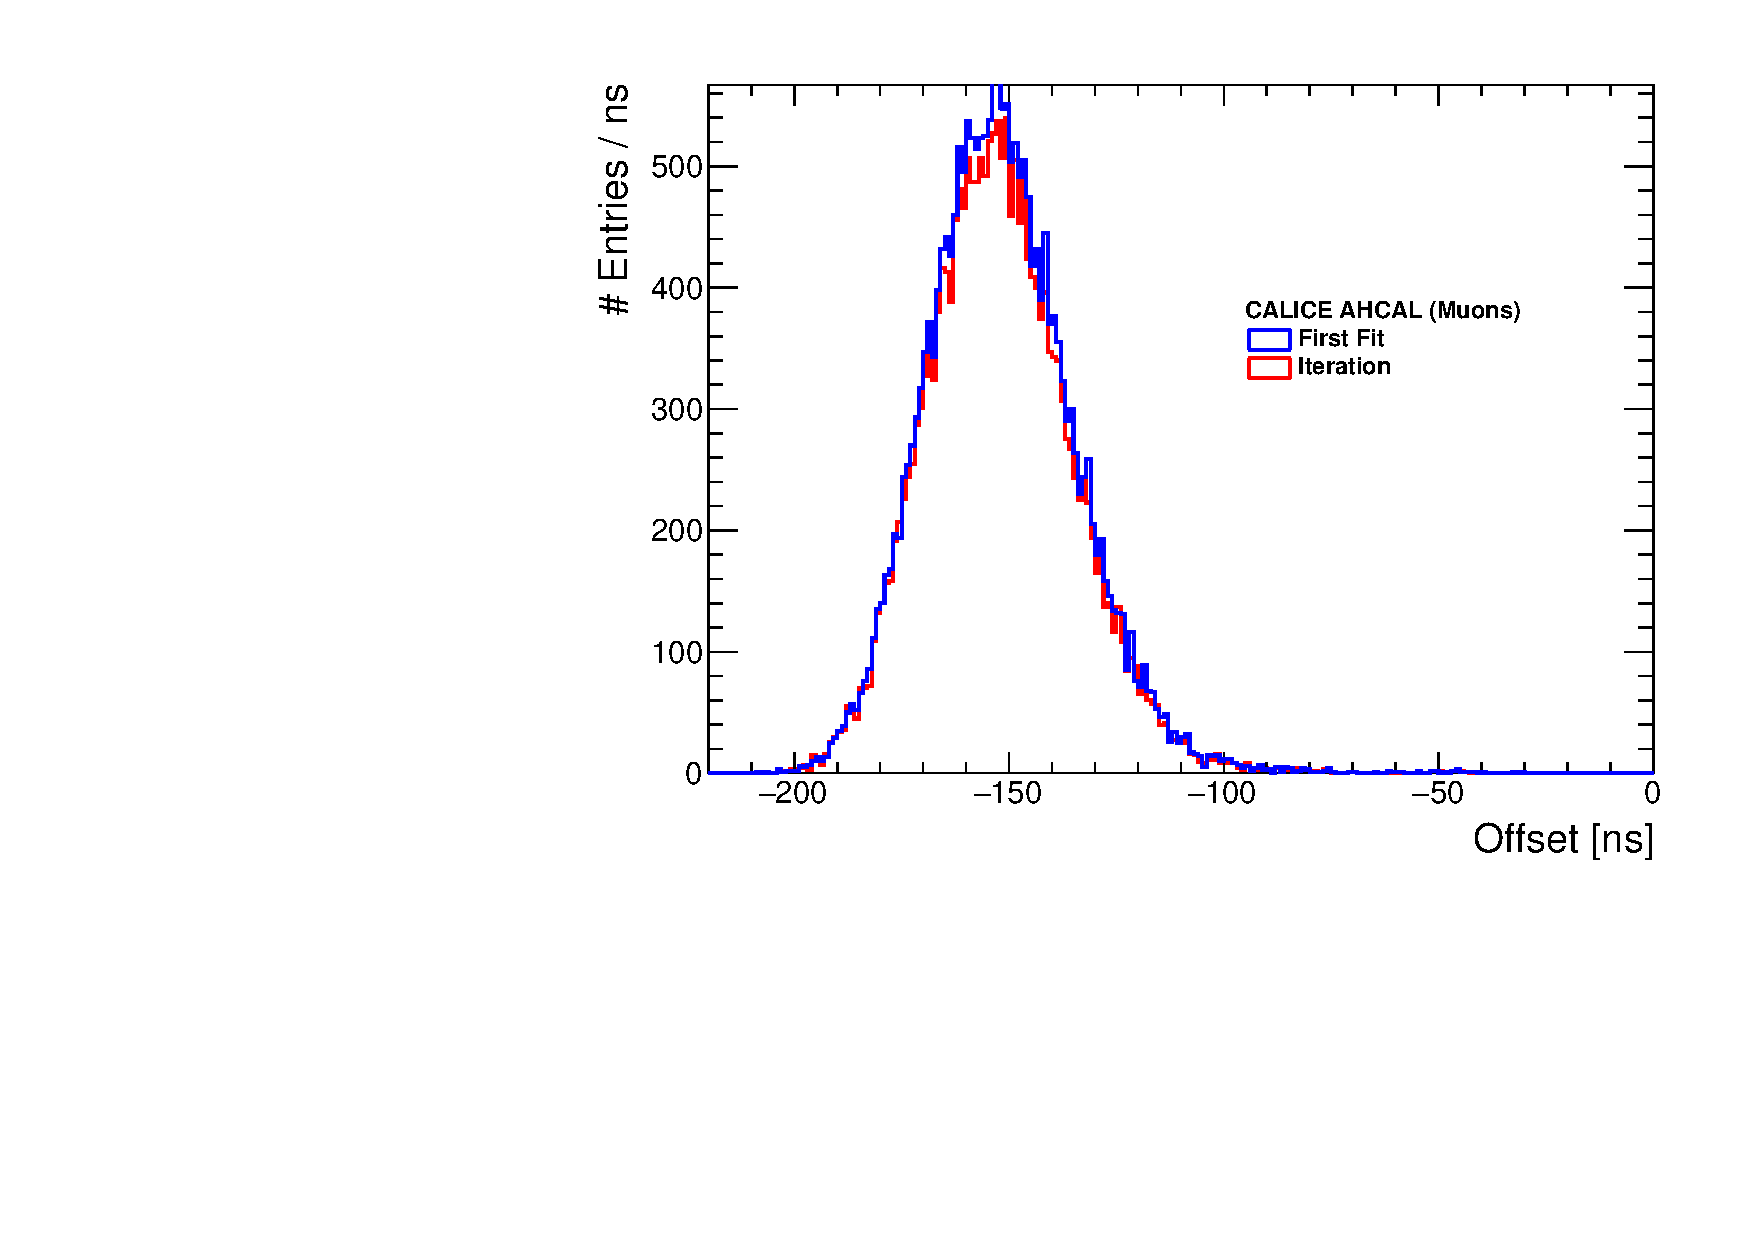
\includegraphics[width=1\textwidth]{chap5/fig_AHCAL_timing/Muons/ExtractedOffsets.pdf}
		\caption{Distribution of the offset used to correct for the trigger delay.}\label{fig:offset_trigger_distribution}
	\end{subfigure}
	\hfill
	\begin{subfigure}[t]{0.45\textwidth}
		\centering
		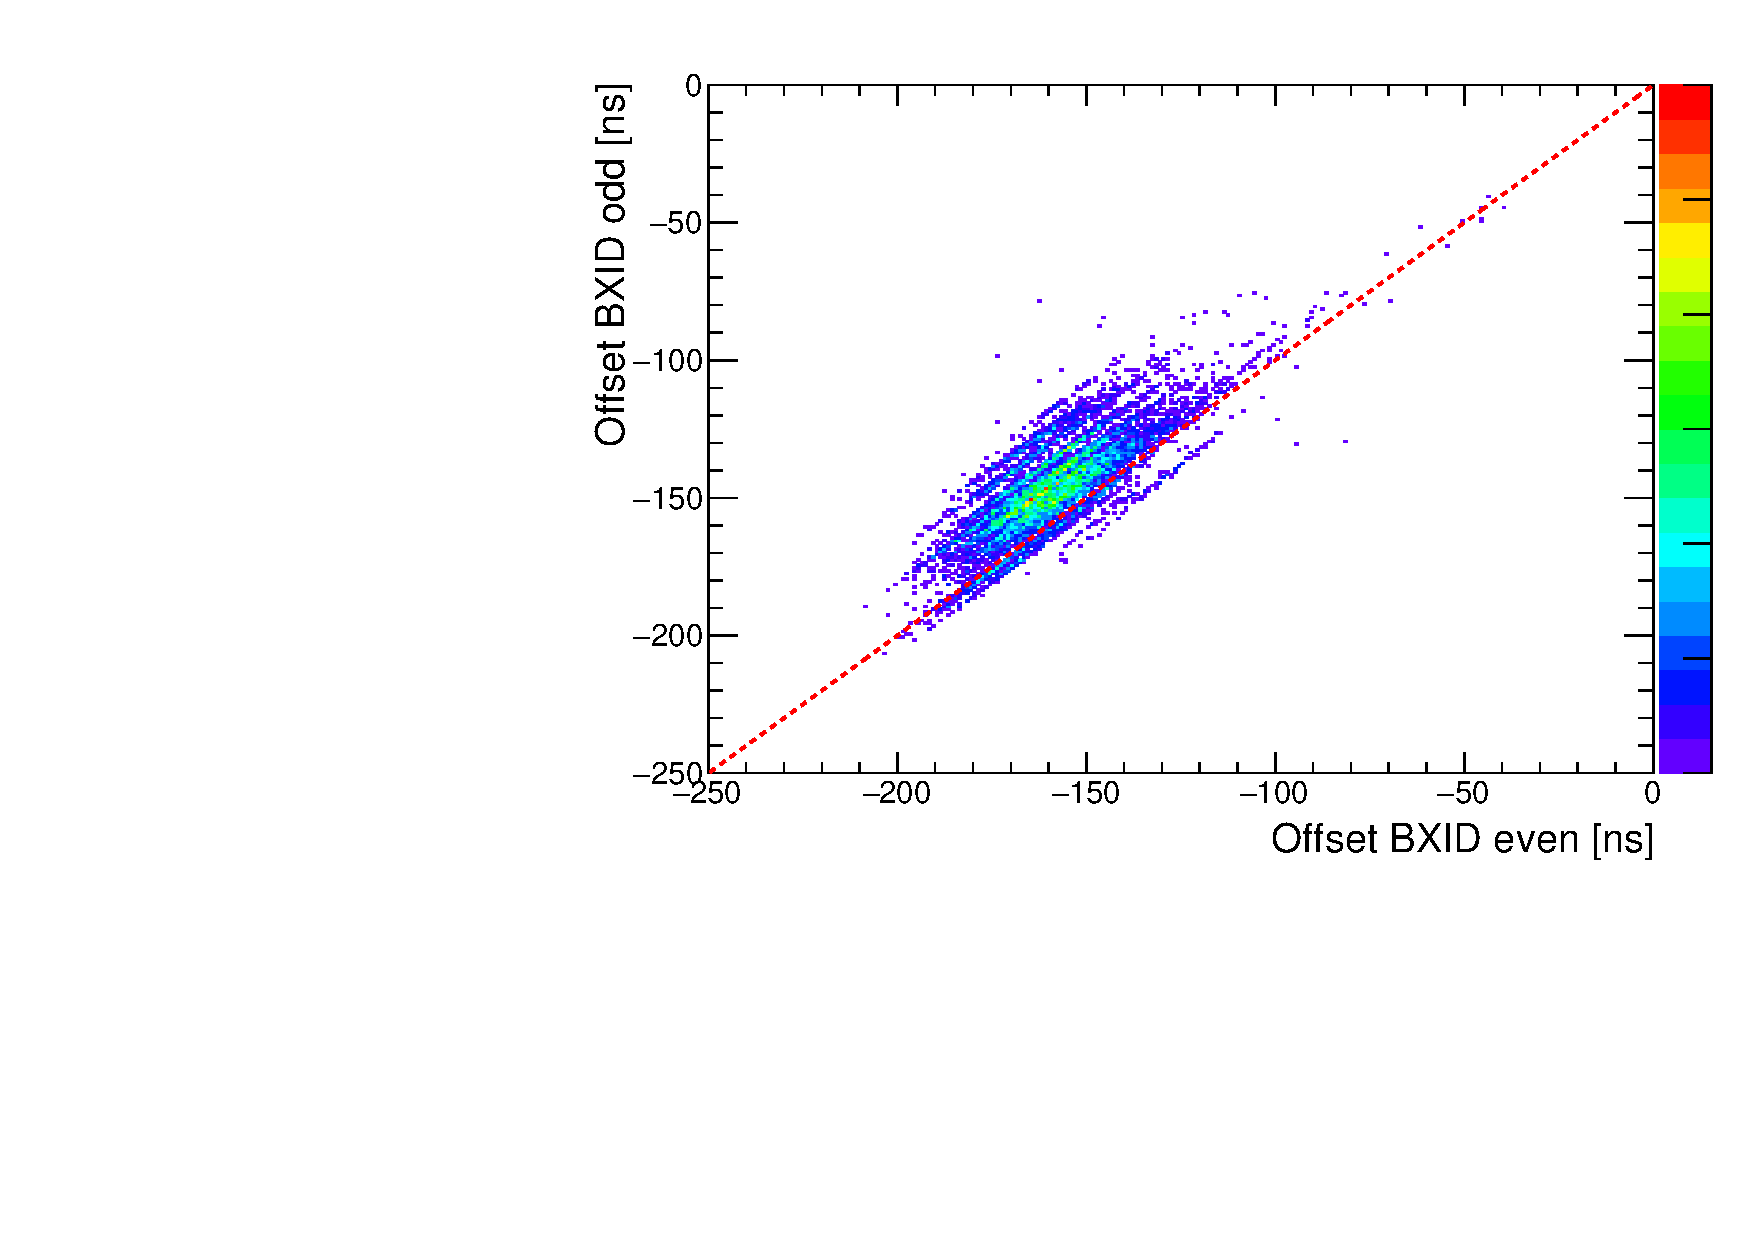
\includegraphics[width=1\textwidth]{chap5/fig_AHCAL_timing/Muons/CorrelationOffsets_BXID.pdf}
		\caption{Correlation between offsets extracted for even and odd BXID.}\label{fig:BXID_offset}
	\end{subfigure}
	\caption{\subref{fig:offset_trigger_distribution} Extracted offset used to correct for the trigger delay signal. The mean delay of the trigger is $\sim$150 ns. \subref{fig:BXID_offset} Correlation between offsets extracted for BXID even and odd.}
\end{figure}

\subsubsection{Time of the first hit distribution}
After the selection, the time of the first hit (T$_{fH}$) can be obtained by plotting the distribution of T$_{chn}$ - T$_{ref}$ as shown in figure \ref{fig:timing_nocorrection}. The combined time resolution (RMS) shown in figure \ref{fig:reso_nocorrection} obtained by combining all layers is around 5.65 ns by just applying the time calibration on the data. Some improvements are possible as described in the subsections \ref{subsec:lin_corr} and \ref{subsec:timewalk}. The discrepancy observed for the layer 11 is most likely due to an electronic problem in the TDC voltage ramp of the chips on that layer.

\begin{figure}[htbp!]
	\begin{subfigure}[t]{0.45\textwidth}
		\centering
		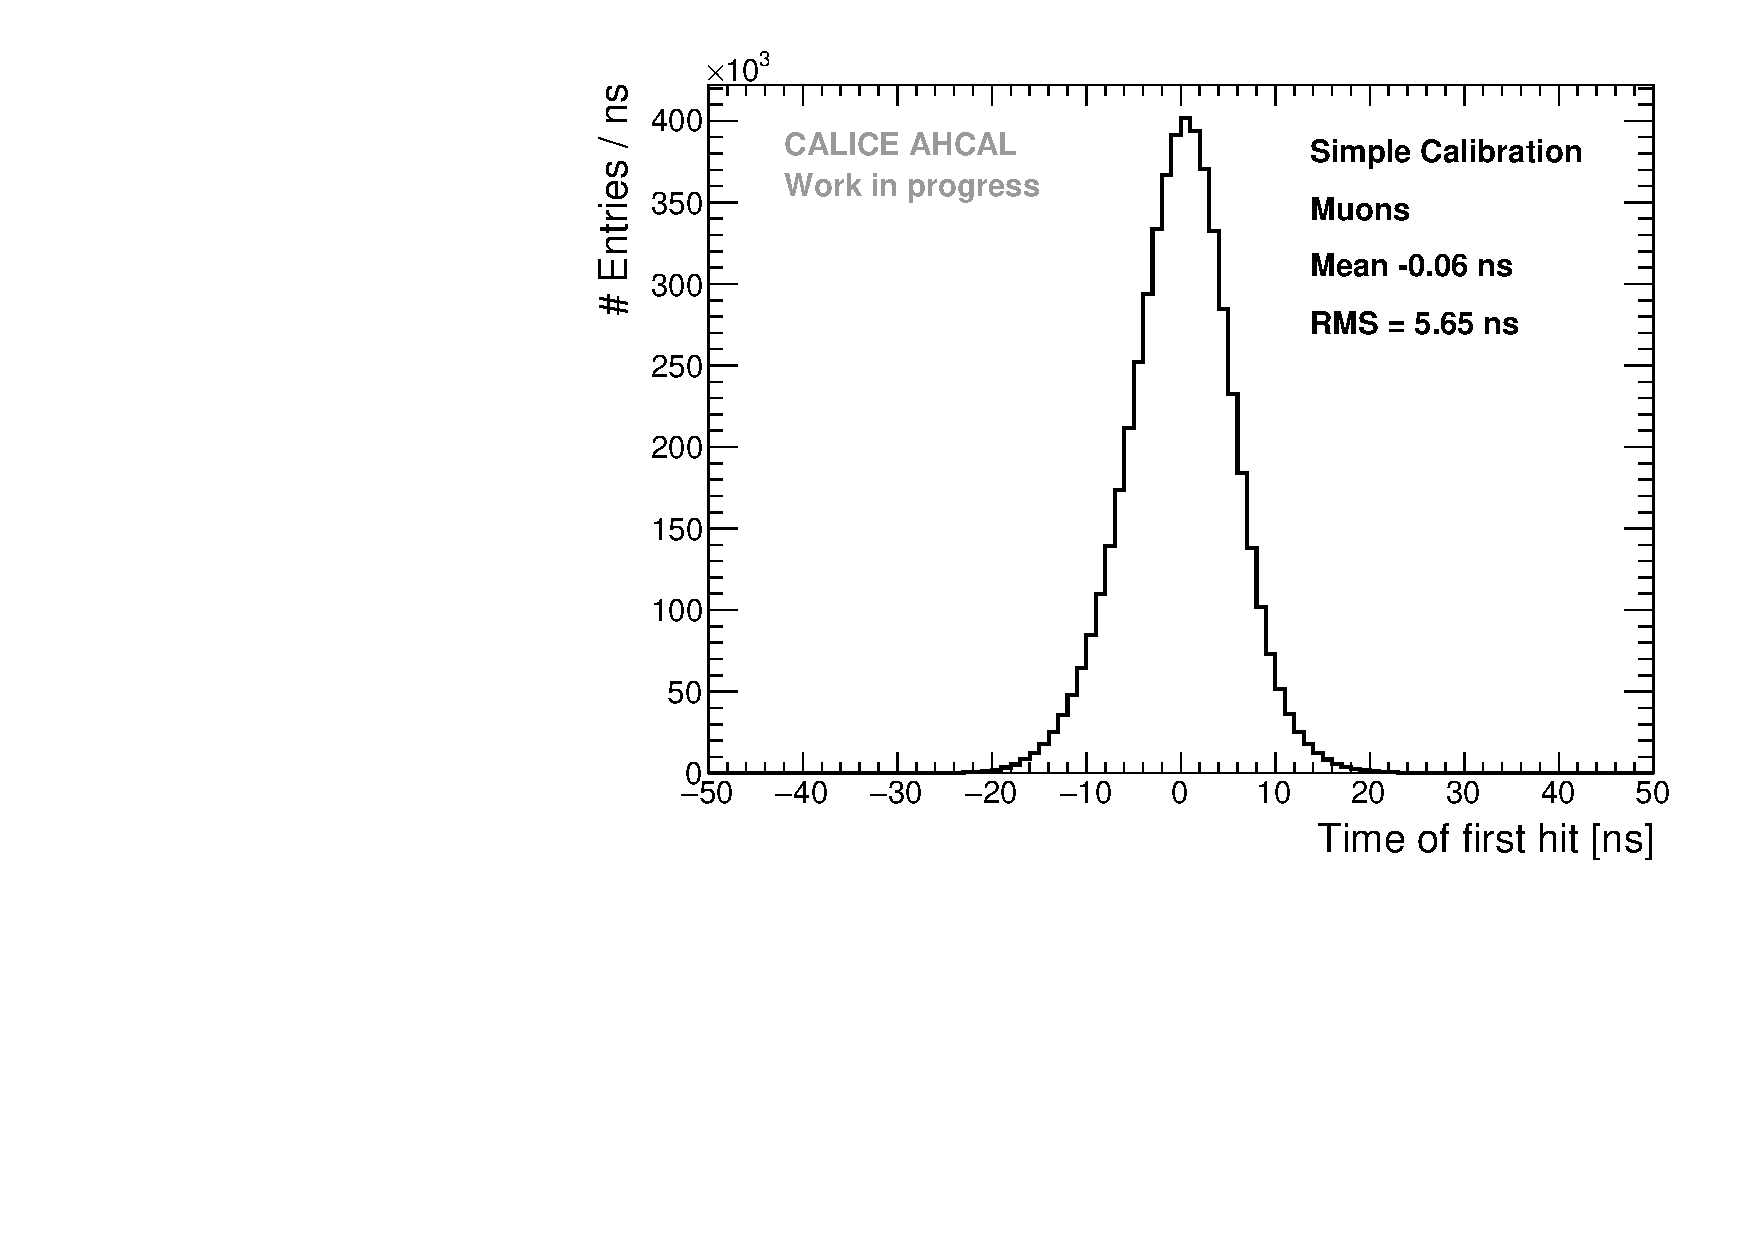
\includegraphics[width=1\textwidth]{chap5/fig_AHCAL_timing/Muons/Timing_AHCAL_noCorrections.pdf}
		\caption{Timing for all layers in the AHCAL.}\label{fig:timing_nocorrection}
	\end{subfigure}
	\hfill
	\begin{subfigure}[t]{0.45\textwidth}
		\centering
		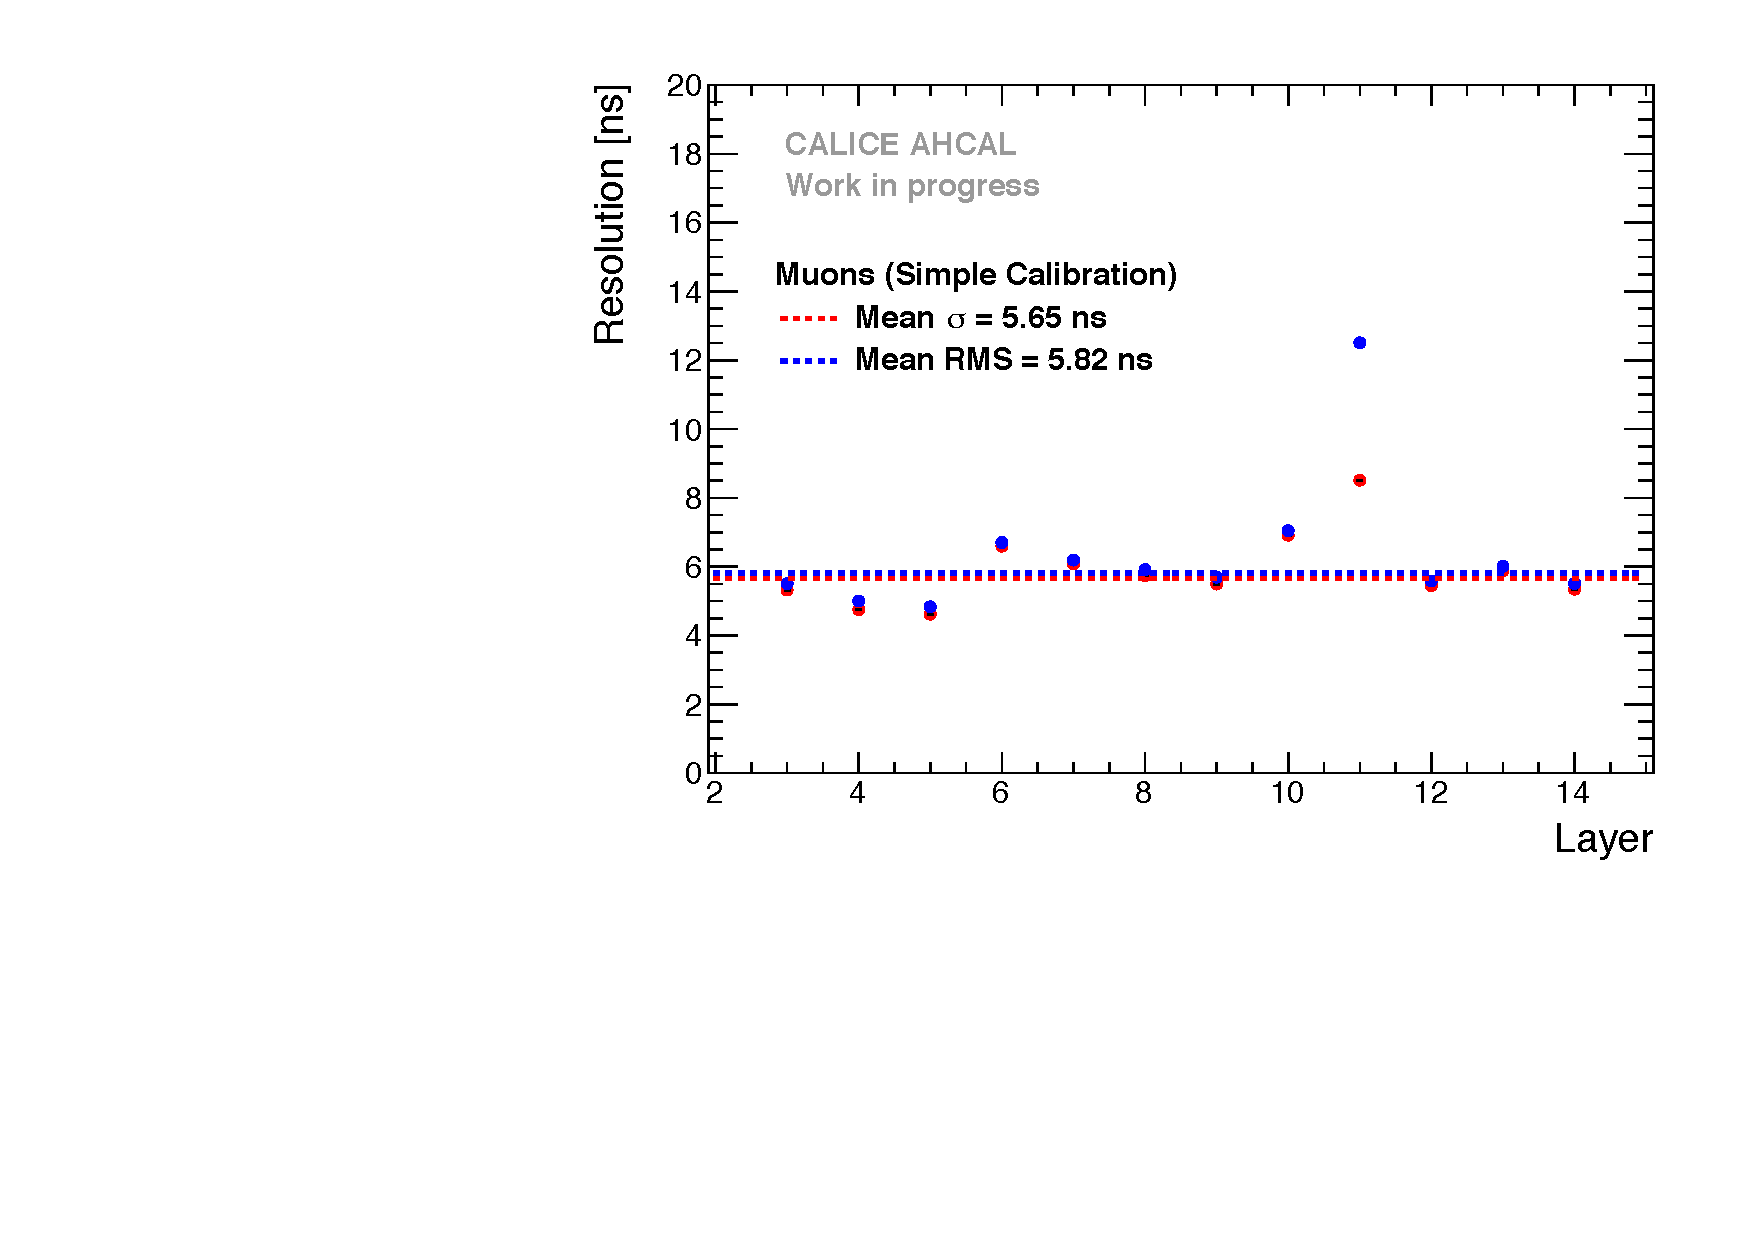
\includegraphics[width=1\textwidth]{chap5/fig_AHCAL_timing/Muons/ResolutionPerModule_noCorrections.pdf}
		\caption{Extracted resolution for all layers in the AHCAL.}\label{fig:reso_nocorrection}
	\end{subfigure}
	\caption{\subref{fig:timing_nocorrection} Time of the first hit distribution of the AHCAL after the first part of the calibration. $\mu$ = -0.06 ns , RMS = 5.65 ns. The distribution is clearly asymmetric. \subref{fig:reso_nocorrection} Time resolution for all layers in the AHCAL. The mean RMS is 5.65 ns.}
\end{figure}

\subsection{Corrections applied to data}
\subsubsection{Ramp non-linearity correction}
\label{subsec:lin_corr}

The calibration relies on the linearity of the TDC voltage ramp in the SPIROC2b by measuring the minimum and maximum of the ramp and interpolating assuming a linear ramp. This assumption is not entirely reliable as described in \cite{OskarSSP, EldwanSSP}. For this, a correction of the non-linearity has to be applied. By simply looking at the time of the first hit (T$_{fH}$) for each chip and BXID versus the TDC value of the hit, the shape of the graph would indicate how reliable is the assumption. Indeed if the ramp would be perfectly linear, one would obtain a flat graph. A quadratic fit is performed for each chip and BXID in order to correct for the non-linearity of the ramp as shown in figure \ref{fig:LinCorr}. A check has been performed on the quality of the correction, seen in figure \ref{fig:LinCorr_2}. The non-linearity correction results in an improvement on the timing resolution (RMS) of the AHCAL of $\sim$5.1\% (5.36 ns) as shown in figure \ref{fig:timing_lincorrection}.

\begin{figure}[htbp!]
	\begin{subfigure}[t]{0.45\textwidth}
		\centering
		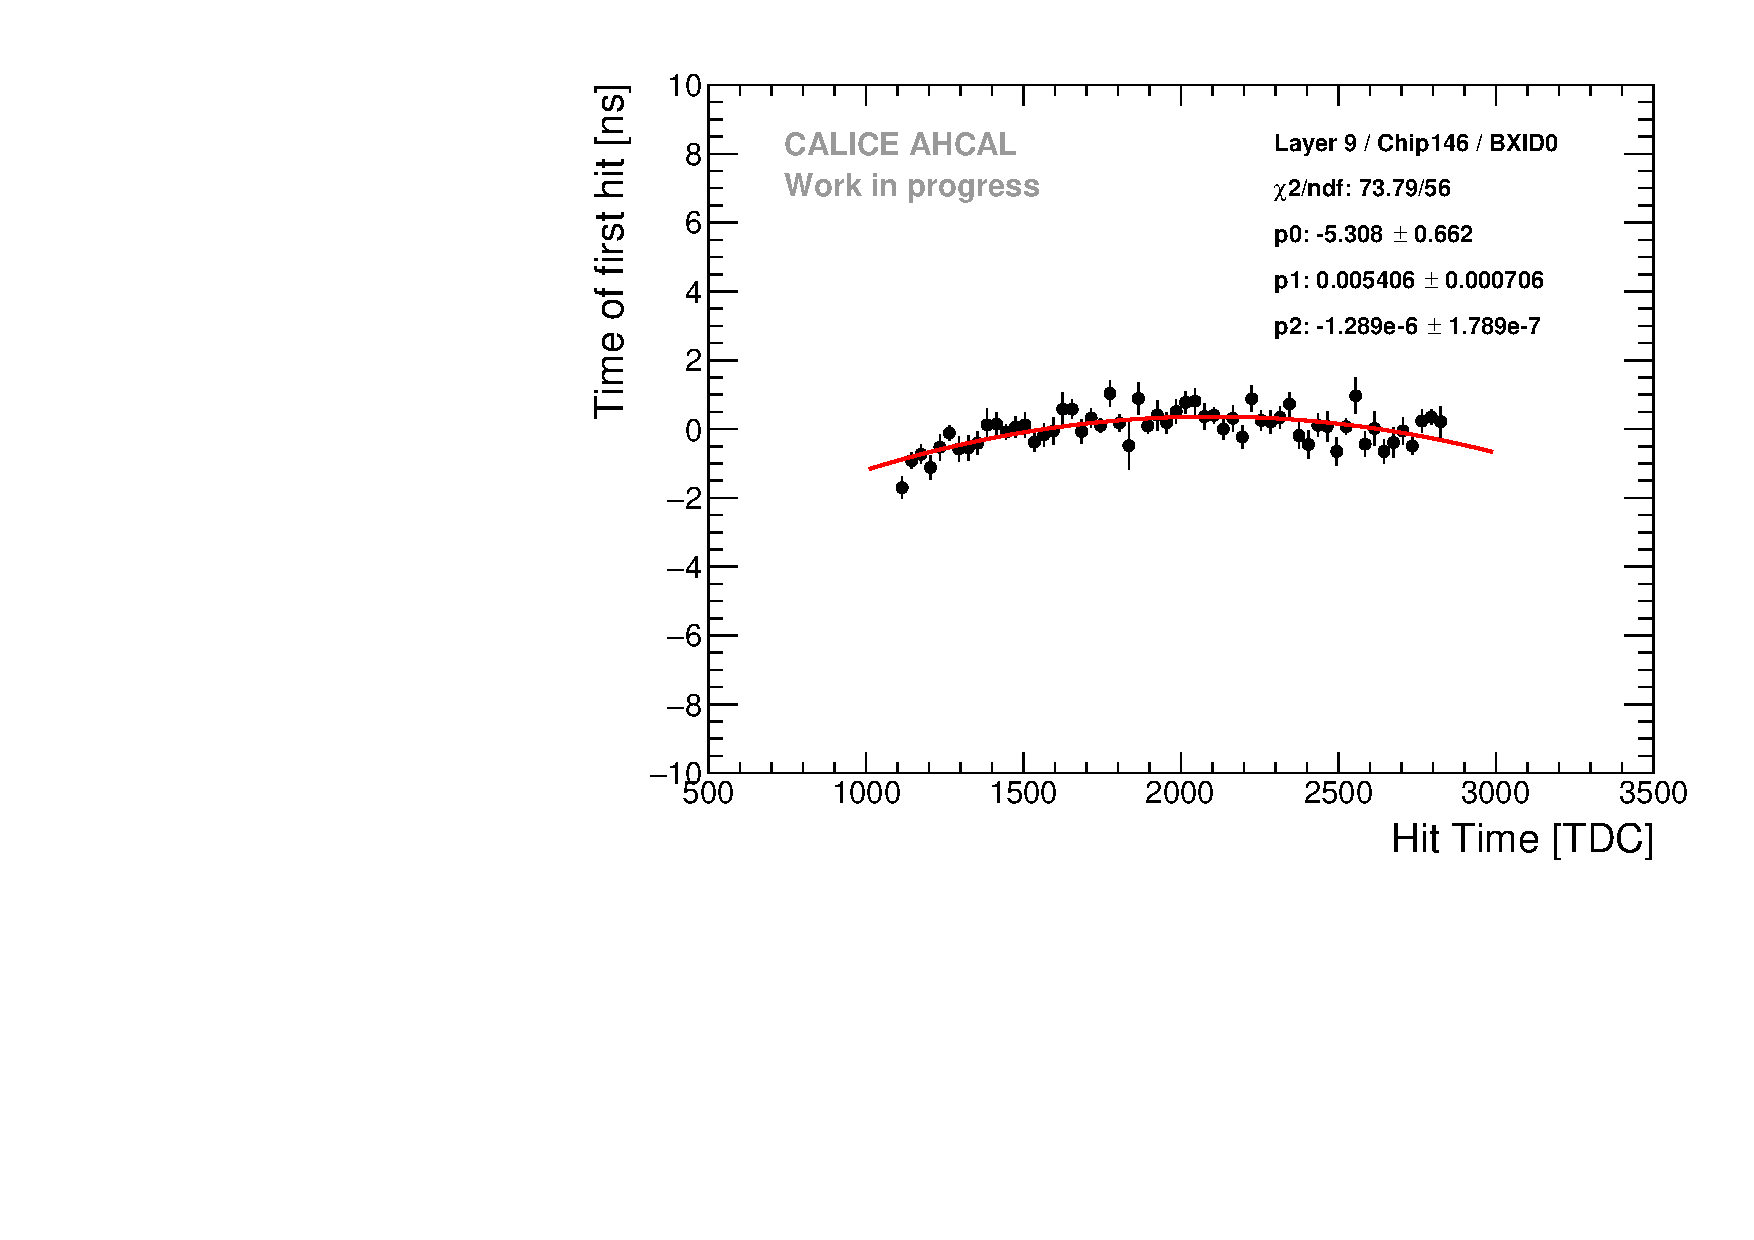
\includegraphics[width=1\textwidth]{chap5/fig_AHCAL_timing/Muons/LinearityCorrection_Module09_Chip146_BXID0.pdf}
		\caption{Quadratic fit of chip 146 (BXID even) on layer 09.}\label{fig:LinCorr}
	\end{subfigure}
	\hfill
	\begin{subfigure}[t]{0.45\textwidth}
		\centering
		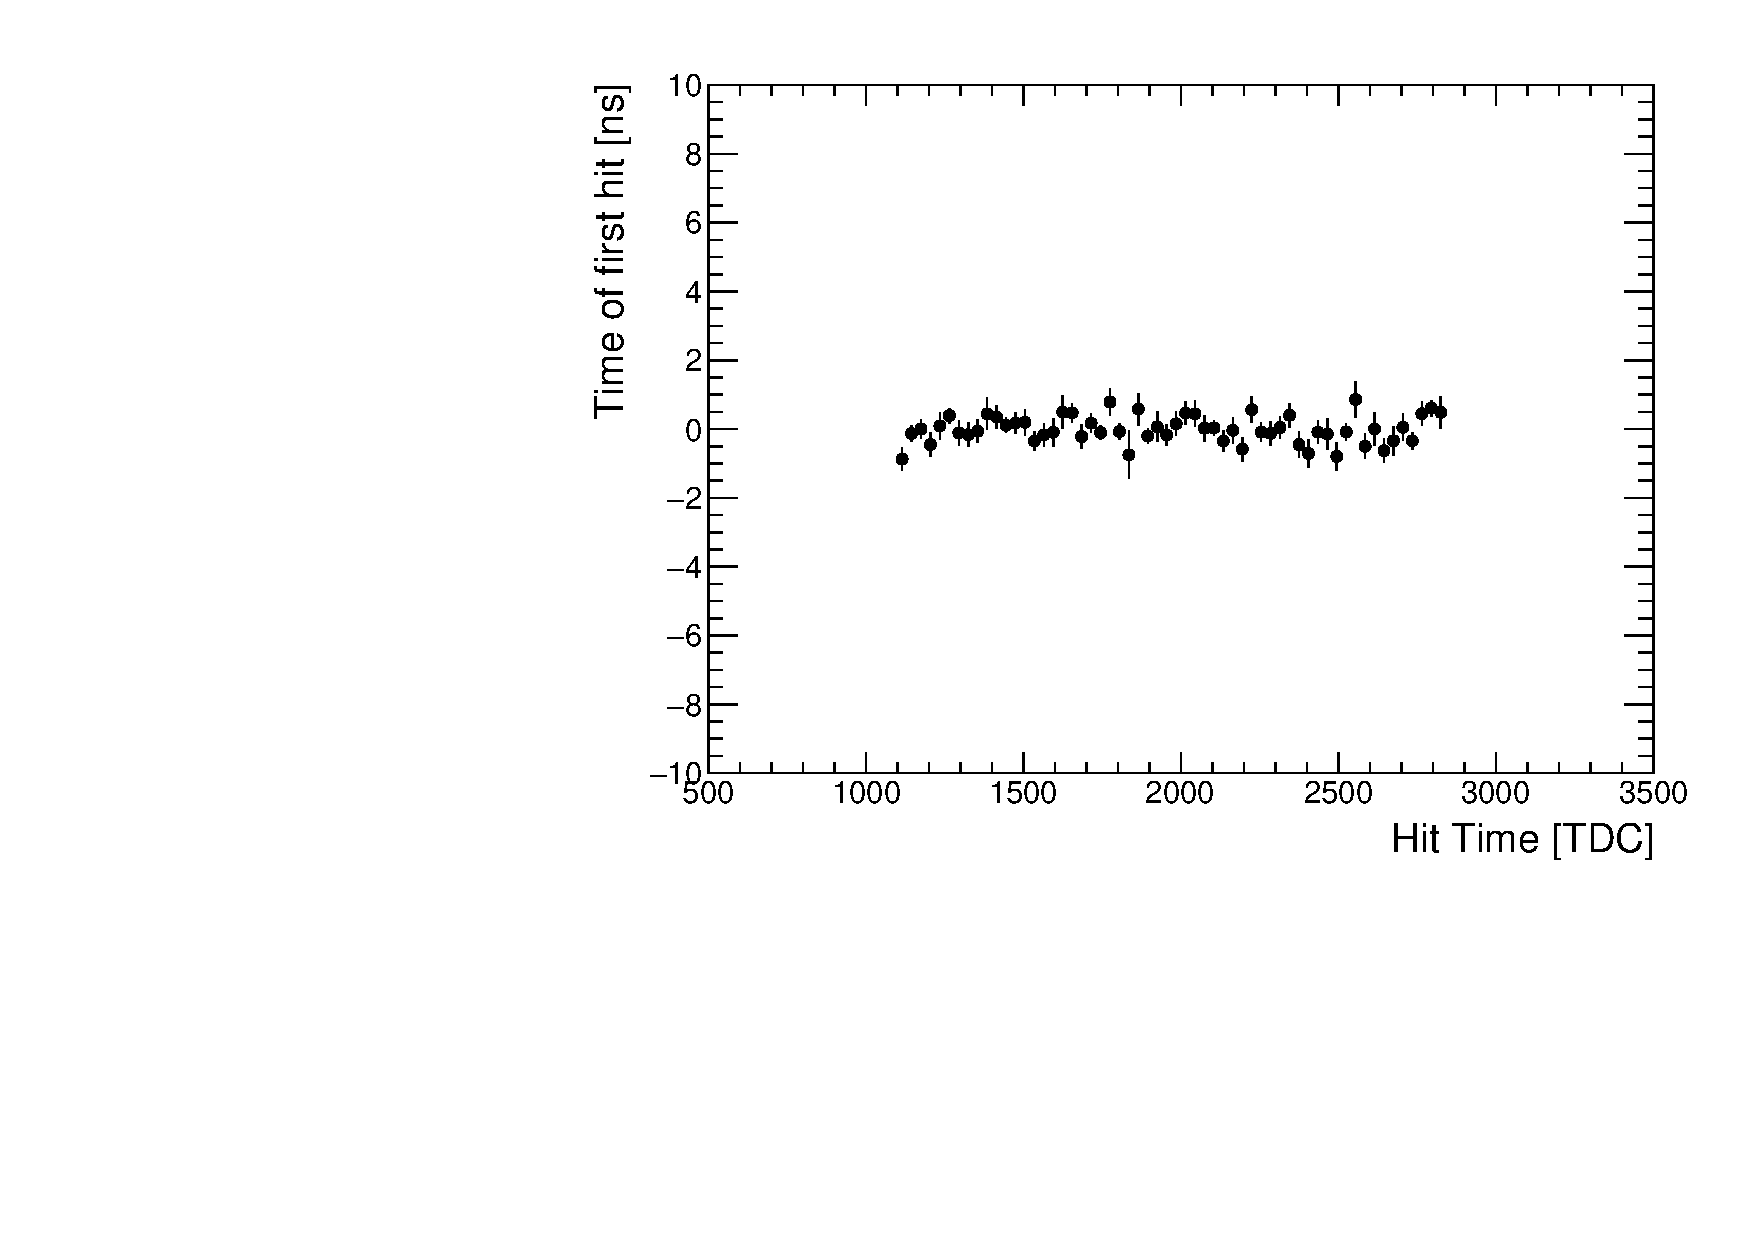
\includegraphics[width=1\textwidth]{chap5/fig_AHCAL_timing/Muons/LinearityCorrection_Module09_Chip146_BXID0_Corrected.pdf}
		\caption{Profile for chip 146 on layer 09 after the non-linearity correction of the ramp.}\label{fig:LinCorr_2}
	\end{subfigure}
	\caption{\subref{fig:LinCorr} The $\chi^2$ of the fit is 1.29. \subref{fig:LinCorr_2} The correction parameter are applied then on the data to cross-check the quality of the correction. One can see that the curve flattens with the correction applied.}
\end{figure}

\begin{figure}[htbp!]
	\begin{subfigure}[t]{0.45\textwidth}
		\centering
		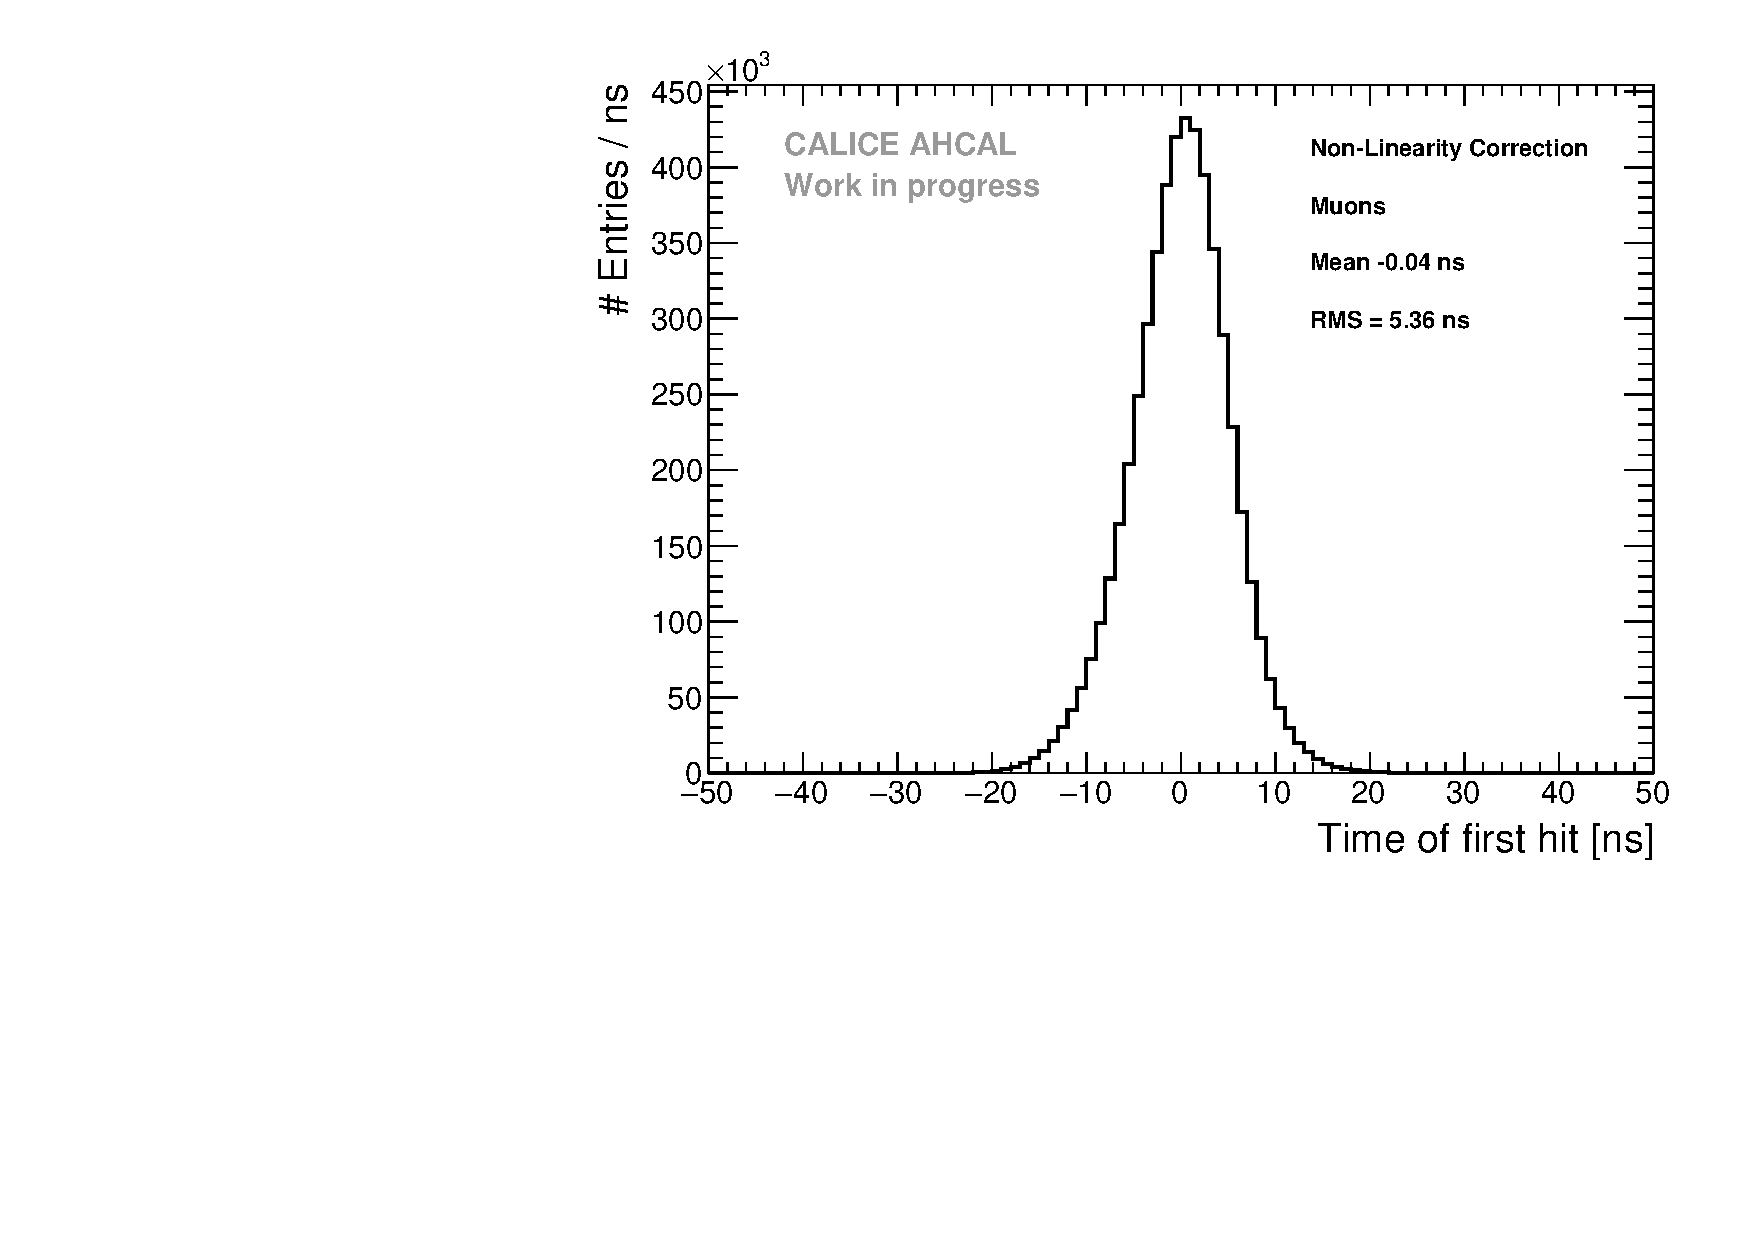
\includegraphics[width=1\textwidth]{chap5/fig_AHCAL_timing/Muons/Timing_AHCAL_LinCorrection.pdf}
		\caption{Timing for all layers in the AHCAL.}\label{fig:timing_lincorrection}
	\end{subfigure}
	\hfill
	\begin{subfigure}[t]{0.45\textwidth}
		\centering
		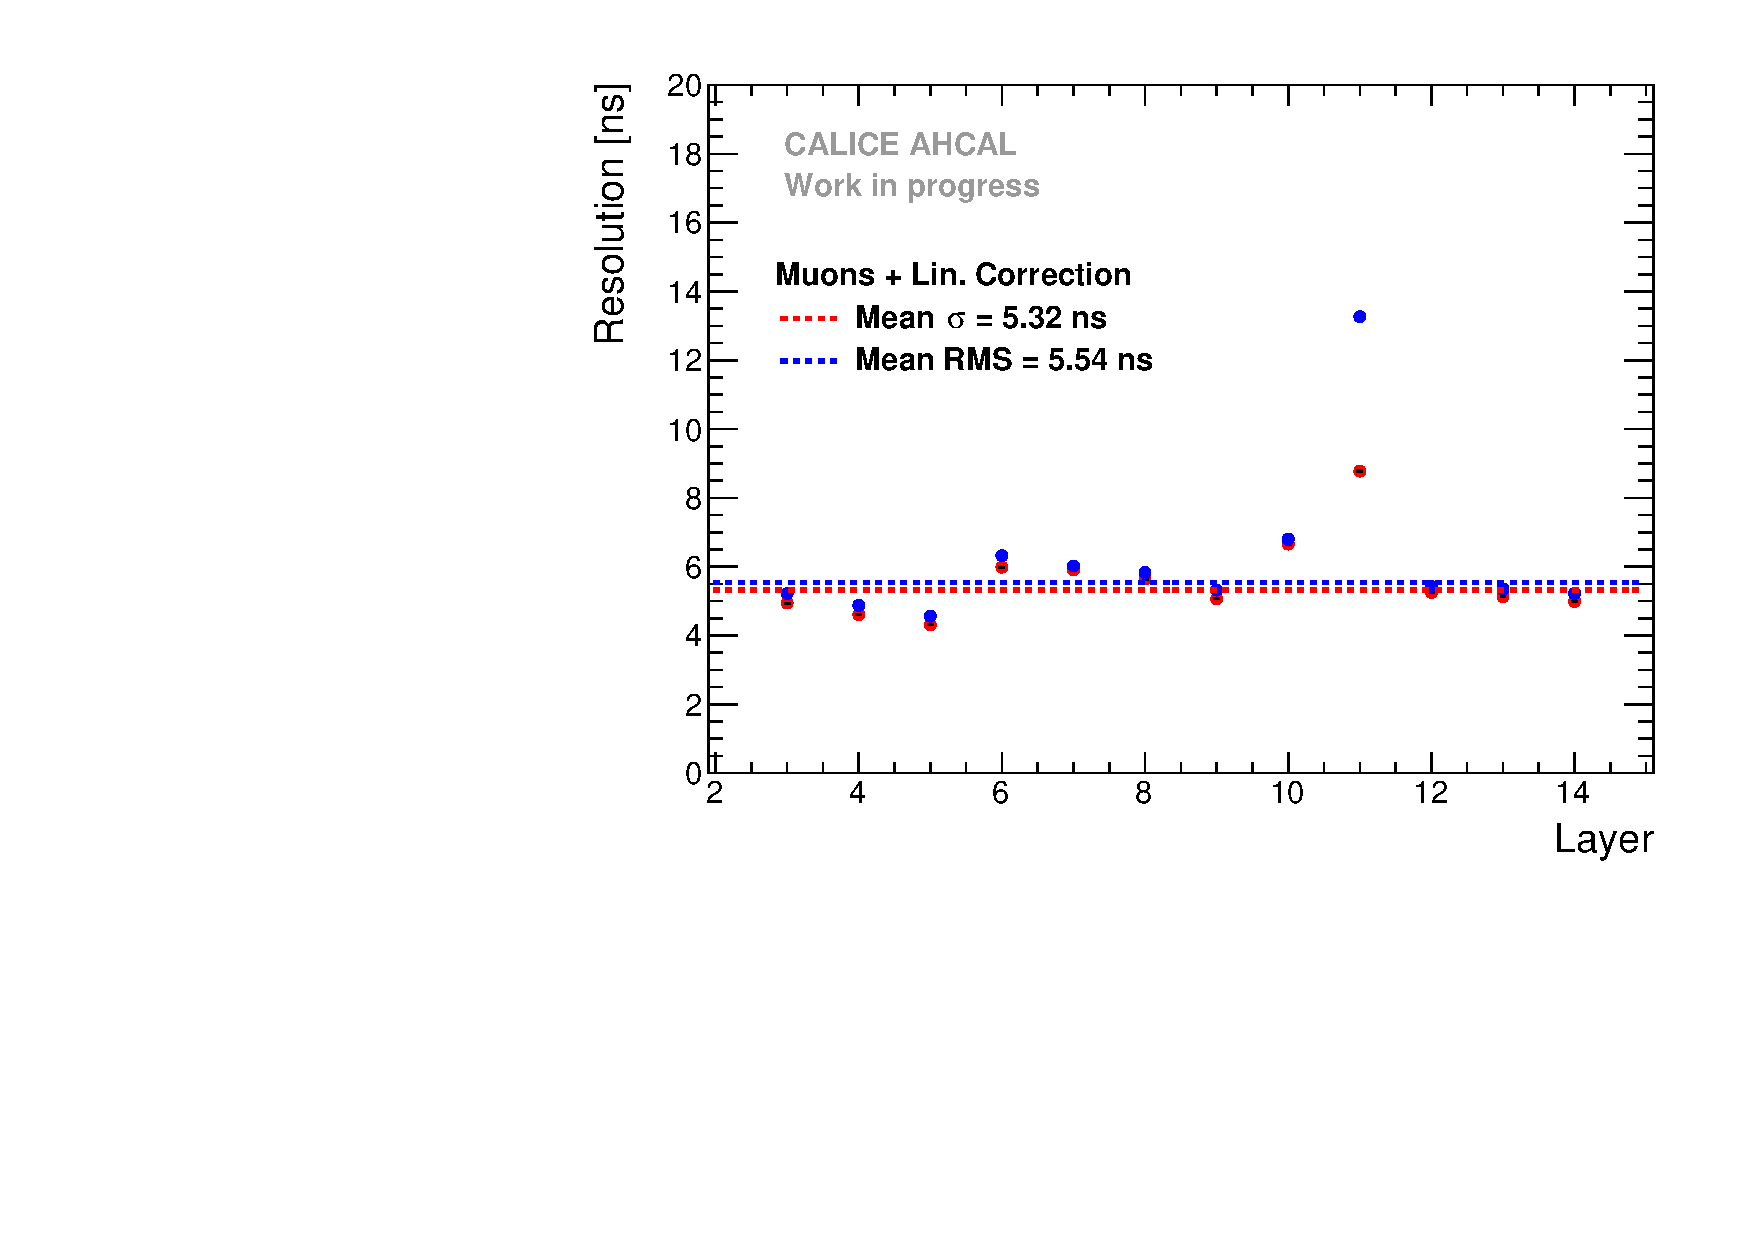
\includegraphics[width=1\textwidth]{chap5/fig_AHCAL_timing/Muons/ResolutionPerModule_LinCorrection.pdf}
		\caption{Extracted resolution for all layers in the AHCAL.}\label{fig:reso_lincorrection}
	\end{subfigure}
	\caption{\subref{fig:timing_lincorrection} Time of the first hit distribution of the AHCAL after the non-linearity correction. $\mu$ = -0.04 ns , RMS = 5.36 ns. \subref{fig:reso_lincorrection} Time resolution for all layers in the AHCAL. The mean RMS is 5.54 ns.}
\end{figure}

\subsubsection{Time Walk correction}
\label{subsec:timewalk}

The time-walk effect is due to the presence of a threshold that induces a time shift between a small amplitude signal and a high amplitude signal. Small amplitude signals will systematically trigger at a later time than high amplitude signals. A correction can be applied on the data by looking at the time of the first hit versus the amplitude of the hit. This might be particularly important for late neutrons signals that generally deposit very little energy in the calorimeter. The correction is assumed to be the same for all the chips, independent of the position of the threshold of each chip, as hits are cut at 0.5 MIP and most of the chips were having the threshold set-up well below 0.5 MIP. An exponential fit of the form $\text{A} \times e^{-\lambda{}x} + \text{B}$ is performed on the data to extract the parameters needed to correct the time walk effect as shown on figure \ref{fig:time_walk}. The residuals after correction are in the order of few hundreds of picoseconds as seen in figure \ref{fig:time_walk_corr}.

\begin{figure}[htbp!]
	\begin{subfigure}[t]{0.45\textwidth}
		\centering
		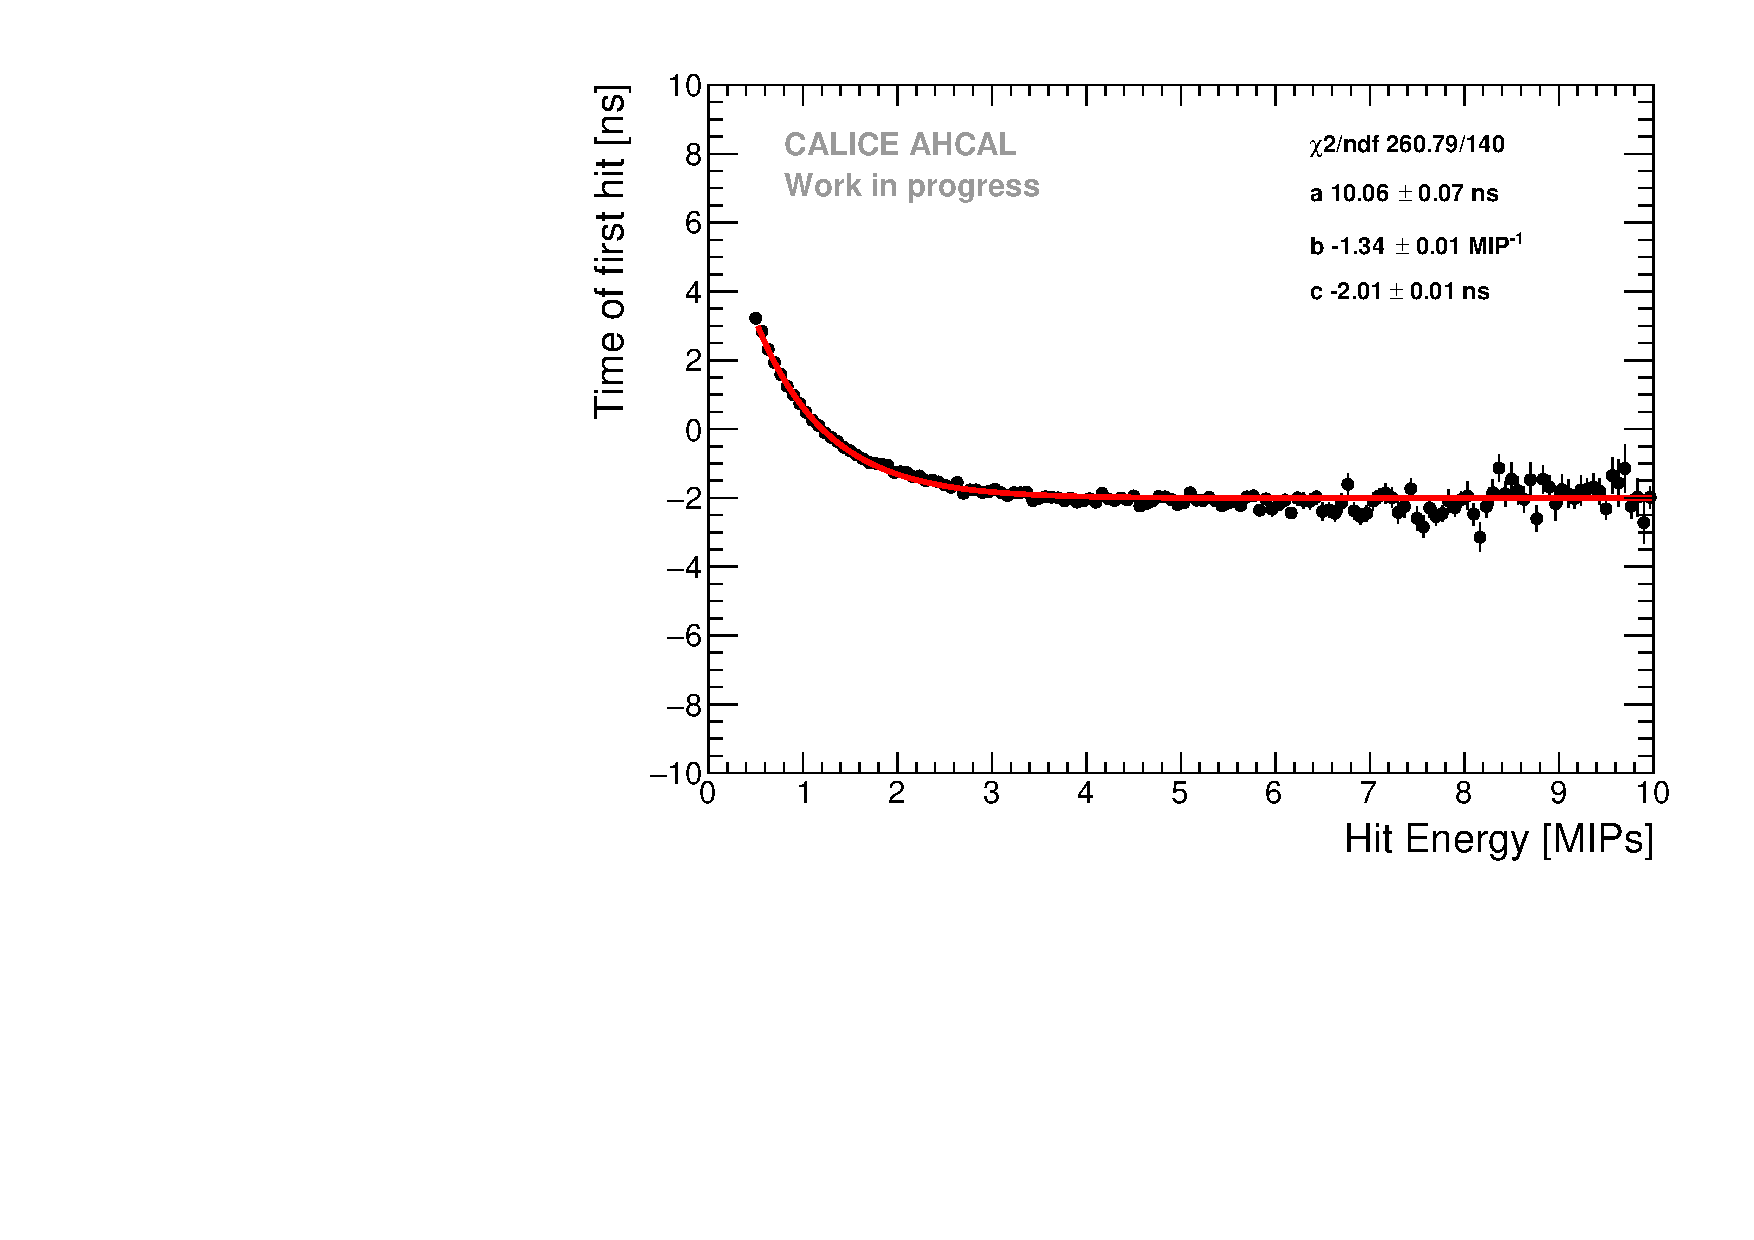
\includegraphics[width=1\textwidth]{chap5/fig_AHCAL_timing/Muons/TimeWalkProfile.pdf}
		\caption{Profile of the time of first hit as function of the hit energy.}\label{fig:time_walk}
	\end{subfigure}
	\hfill
	\begin{subfigure}[t]{0.45\textwidth}
		\centering
		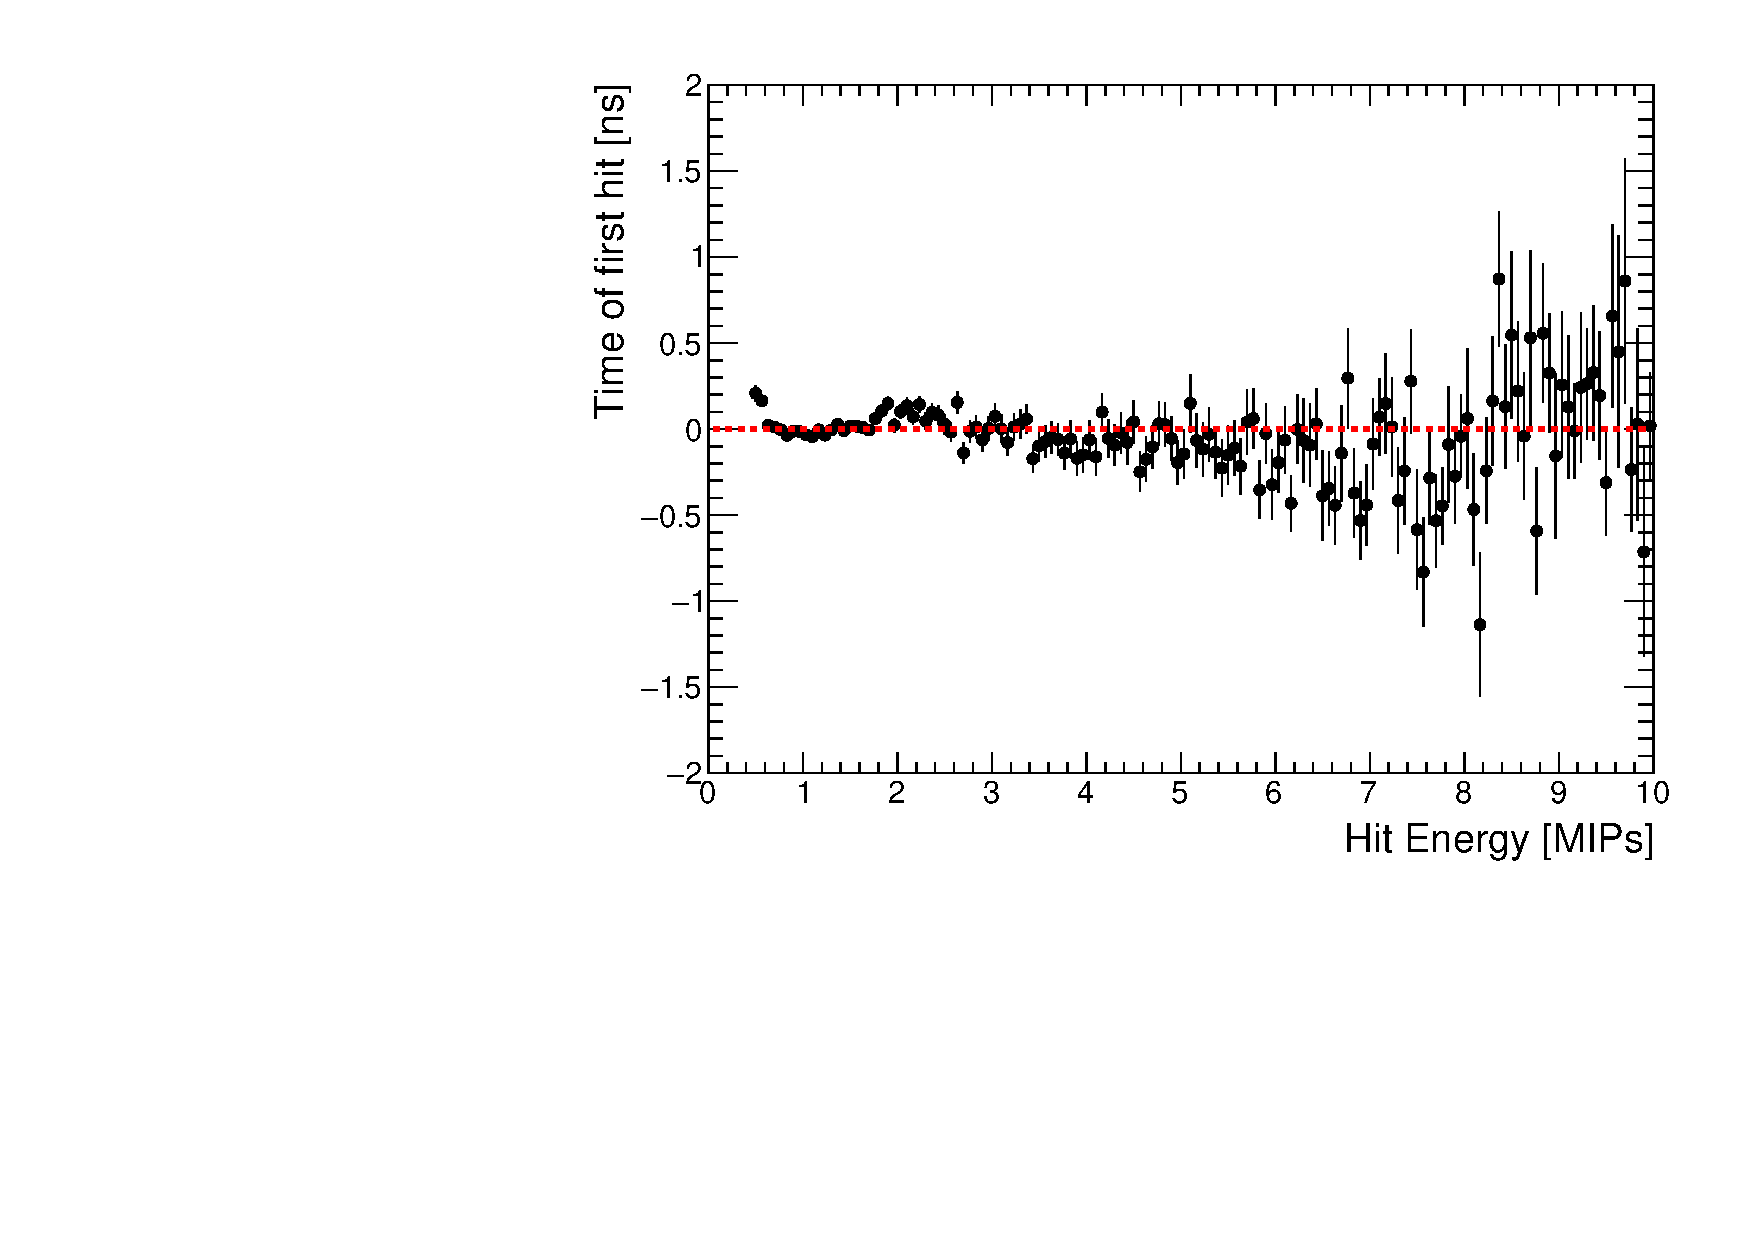
\includegraphics[width=1\textwidth]{chap5/fig_AHCAL_timing/Muons/TimeWalkProfile_Correction.pdf}
		\caption{Same profile after time-walk correction.}\label{fig:time_walk_corr}
	\end{subfigure}
	\caption{\subref{fig:time_walk} Time-walk correction extracted from data. A = 10.06 $\pm$ 0.07, $\lambda$ = -1.34 $\pm$ 0.01, B = -2.01 $\pm$ 0.01. A difference up to 6 ns is seen between small and large amplitudes. \subref{fig:time_walk_corr} Time-walk profile after correction showing a spread of less than 1 ns.}
\end{figure}

\subsubsection{Time of first hit for muons}
\label{subsec:Muon_final}

After the time-walk correction, an improvement of $\sim$3\% can be achieved on the time resolution of the AHCAL (RMS 5.20 ns) as shown in figure \ref{fig:timing_muons}. The figure \ref{fig:timing_reso_all_muons} shows the time resolution obtained in the complete AHCAL. The obtained time resolution is around 5 ns. The distribution is still asymmetric, it is most likely coming from the non-linearity of the TDC ramp of the trigger reference as no external time is available to correct for it. This is taken into account in the simulation by parametrising the time distribution with a double Gaussian function. The number of events identified later than 5$\sigma$ ($\sim$25 ns) is around 1.22\% giving us a good assessment of the noise suppression for muons.

\begin{figure}[htbp!]
	\begin{subfigure}[t]{0.45\textwidth}
		\centering
		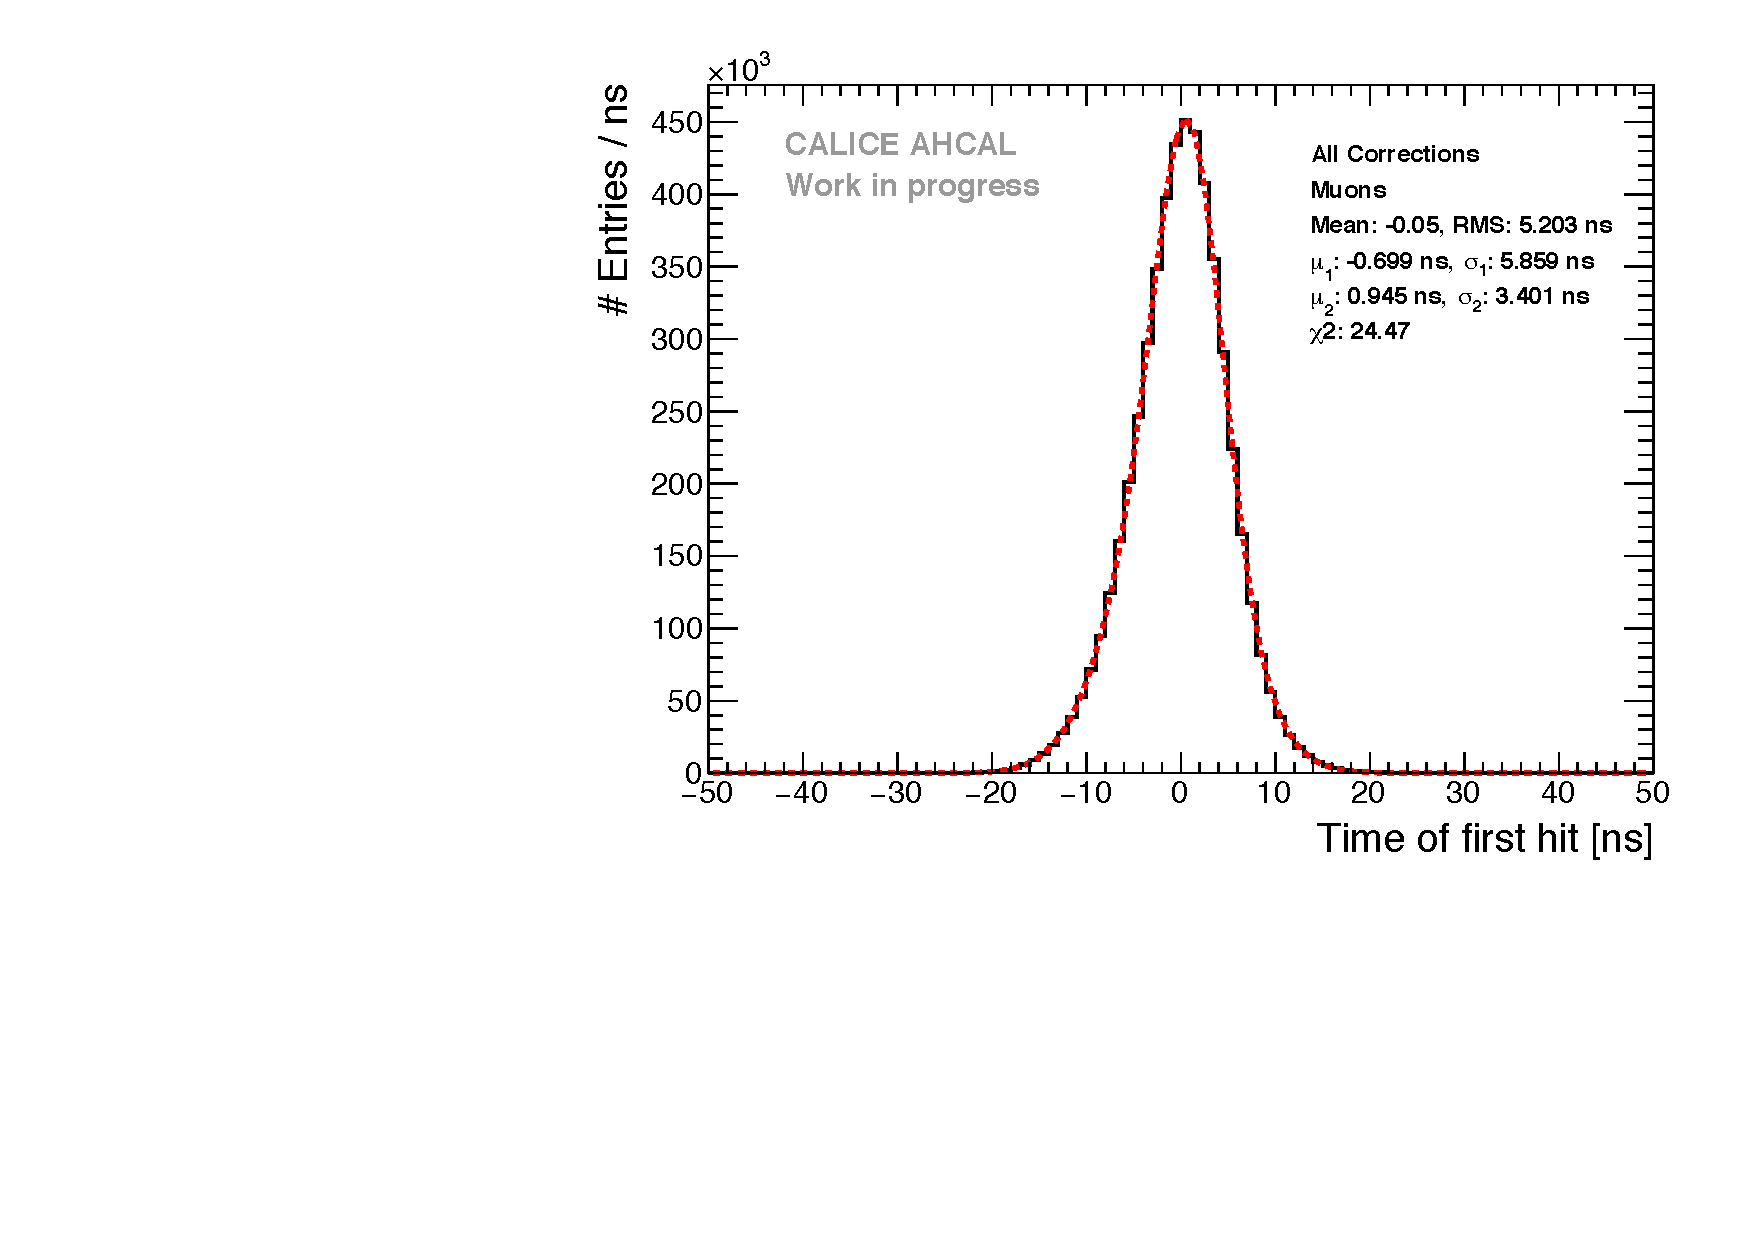
\includegraphics[width=1\textwidth]{chap5/fig_AHCAL_timing/Muons/Timing_AllLayers.pdf}
		\caption{Time of the first hit distribution of the AHCAL after all corrections.}\label{fig:timing_muons}
	\end{subfigure}
	\hfill
	\begin{subfigure}[t]{0.45\textwidth}
		\centering
		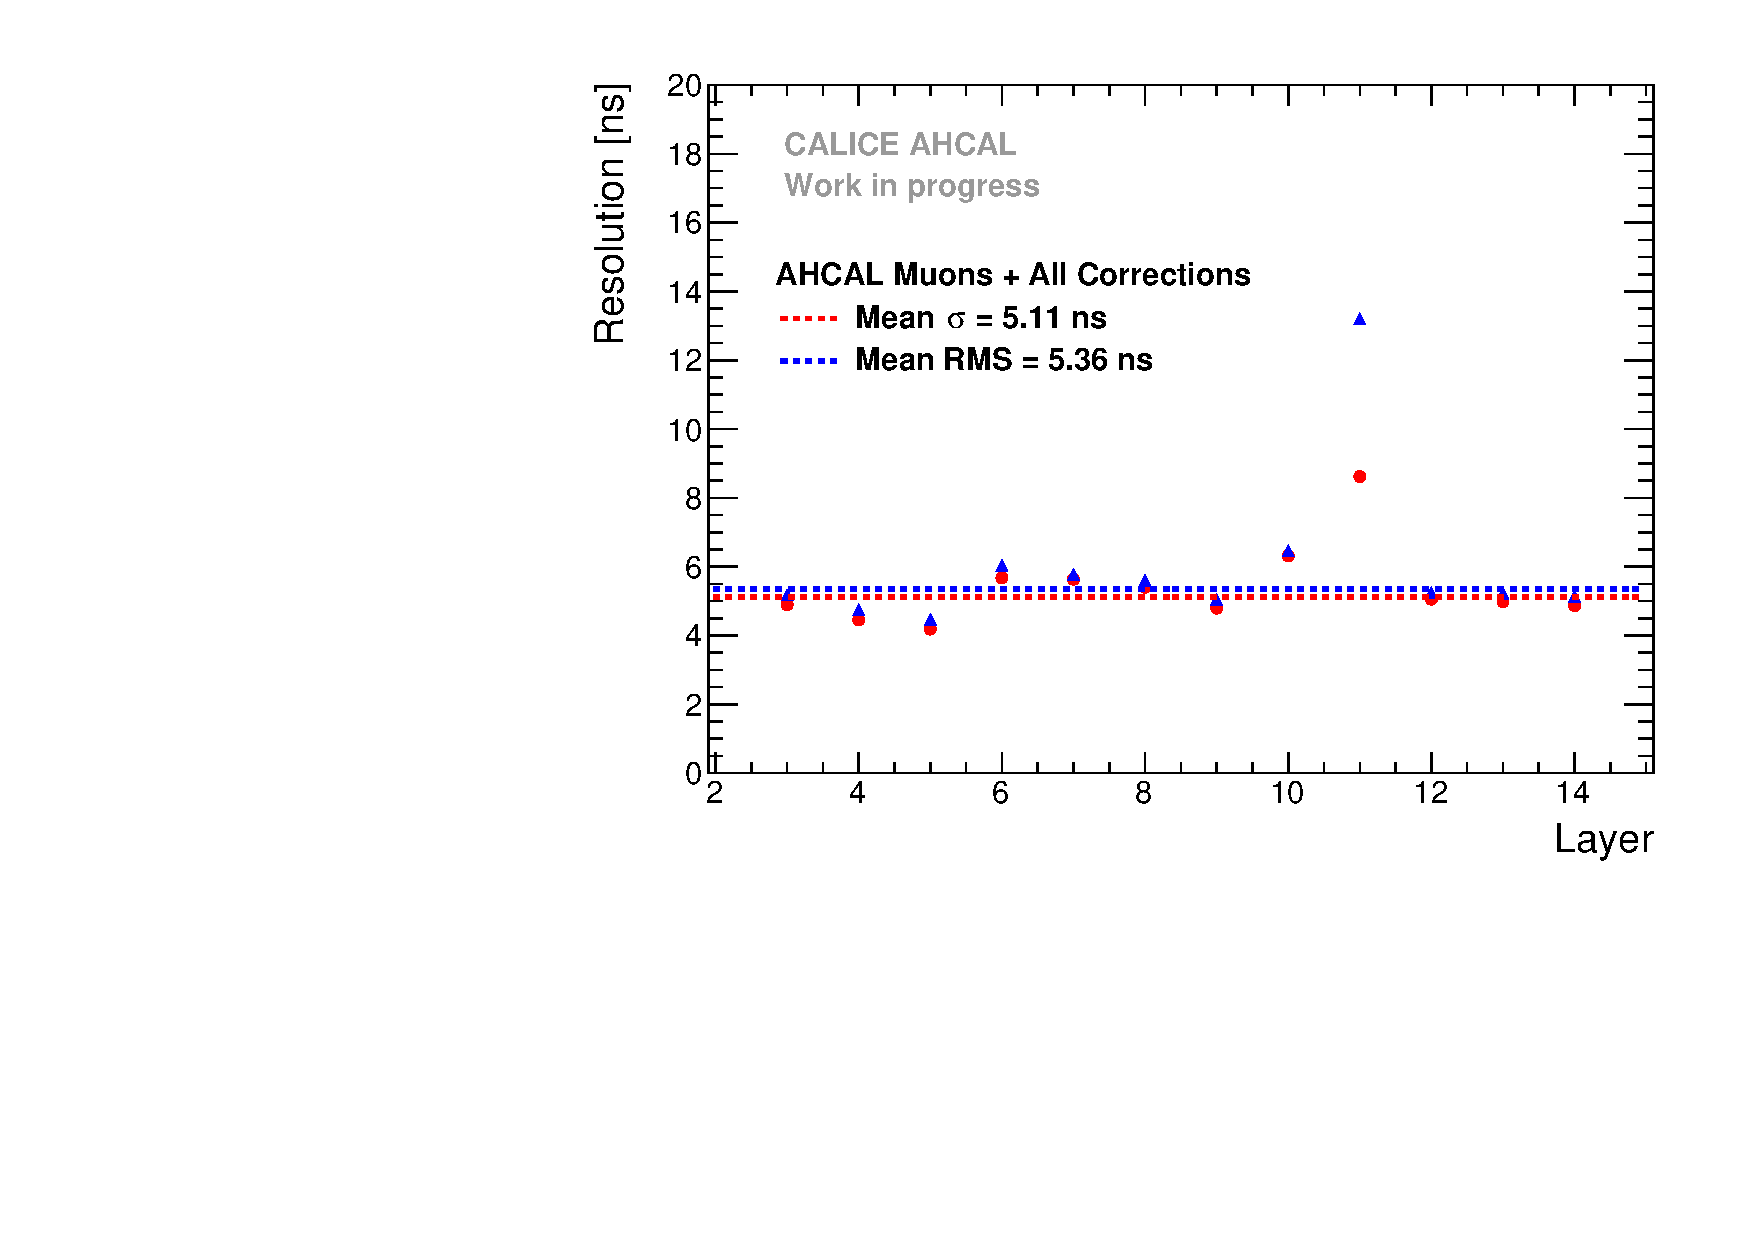
\includegraphics[width=1\textwidth]{chap5/fig_AHCAL_timing/Muons/ResolutionPerModule_AllCorrection.pdf}
		\caption{Time resolution obtained for each AHCAL layers.}\label{fig:timing_reso_all_muons}
	\end{subfigure}
	\caption{\subref{fig:timing_muons} Time of the first hit for muons after all corrections. \subref{fig:timing_reso_all_muons} Time resolution obtained for each layer in the AHCAL. Mean RMS = 5.35 ns.}
\end{figure}

\subsection{Cross-check of the calibration with electrons}
\label{subsec:validation}

In order to validate the calibration, an electron sample is taken. Electromagnetic showers are quasi-instantaneous and perfect to cross-check the time calibration procedure. The selection applied to the data sample is described in subsection \ref{subsec:elec_sel}. The same calibration constants and correction constants are applied to the data except that an additional offset from the trigger signal has to be corrected for. The additional offset is expected to be small as the trigger configuration is very similar to the one for muons. The offset is in the order of 10 ns which is consistent with the changes in trigger configuration. The time of the first hit distribution is shown in figure \ref{fig:Timing_electrons}. The time distribution presents a large tail to the right and is much wider than for muons. This gives a hint that an effect is present in electron data but not in muon data. The difference seen could be related to the fact that in electromagnetic showers, the number of hits is much higher as well as the energy deposited in a single cell can be over hundreds MIP.

\begin{figure}[htbp!]
	\centering
	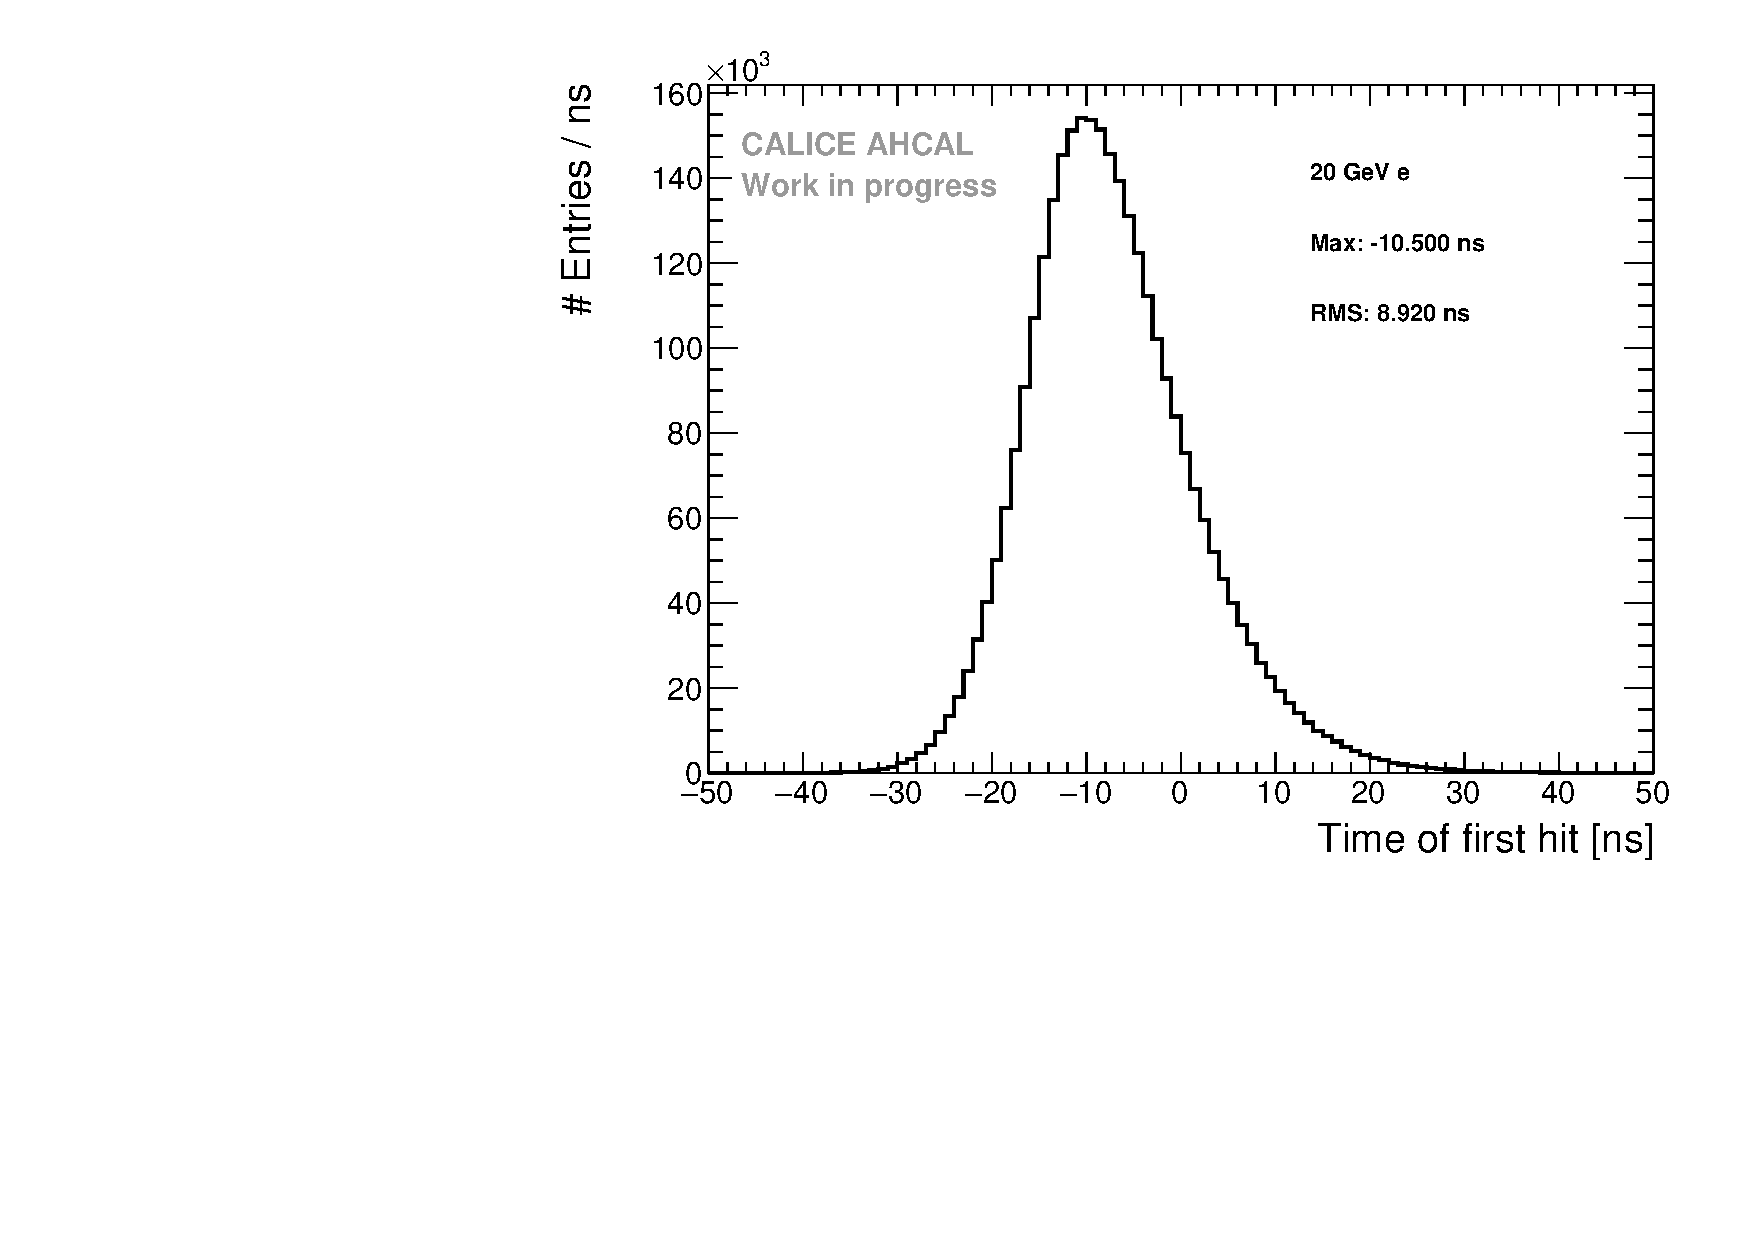
\includegraphics[width=1\textwidth]{chap5/fig_AHCAL_timing/Electrons/Timing_AllLayers_AfterMuons.pdf}
	\caption{Time of the first hit distribution for 20 GeV electrons, Max = 10.05 ns, RMS = 8.92 ns.}
	\label{fig:Timing_electrons}
\end{figure}

\subsection{Influence of the number of triggered channels}
\label{subsec:ped_shift}

Pedestal shift for energy measurement is not a new feature of the SPIROC2b chip \cite{OskarMaster}. This electronic effect may be also present for timing measurement. It can be investigated by looking at the time of the first hit as a function of the number of triggered channels over 0.5 MIP. It is shown in figure \ref{fig:nhits_profile}. This can be drastic on the time measurement of the AHCAL, a correction up to 15-20 ns can be necessary to the data for a high number of trigger. The correction parameters are determined by a linear fit to the data.

\begin{figure}[htbp!]
	\begin{subfigure}[t]{0.45\textwidth}
		\centering
		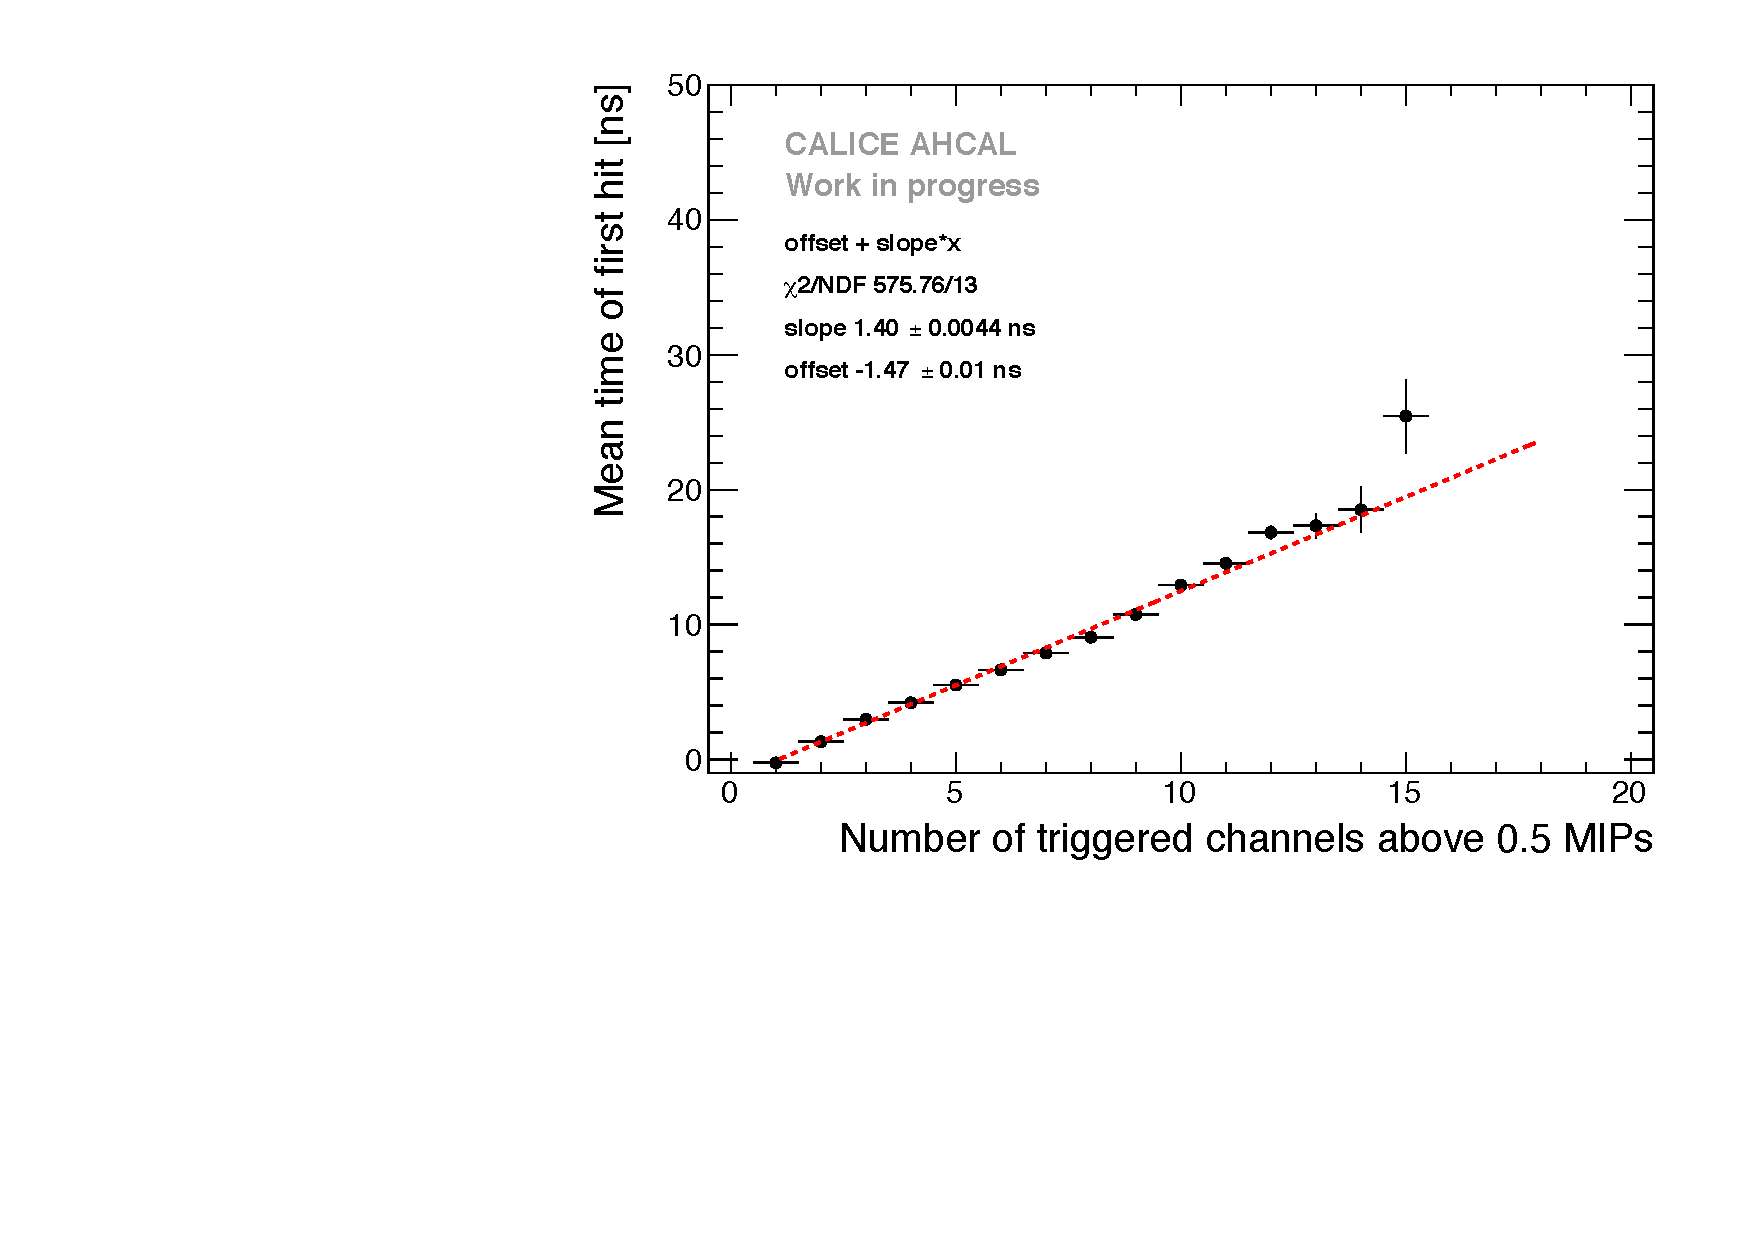
\includegraphics[width=1\textwidth]{chap5/fig_AHCAL_timing/Electrons/NumberHits_Dependance.pdf}
		\caption{Time of the first hit function of the number of triggered channels in a chip (20 GeV).}\label{fig:nhits_profile}
	\end{subfigure}
	\hfill
	\begin{subfigure}[t]{0.45\textwidth}
		\centering
		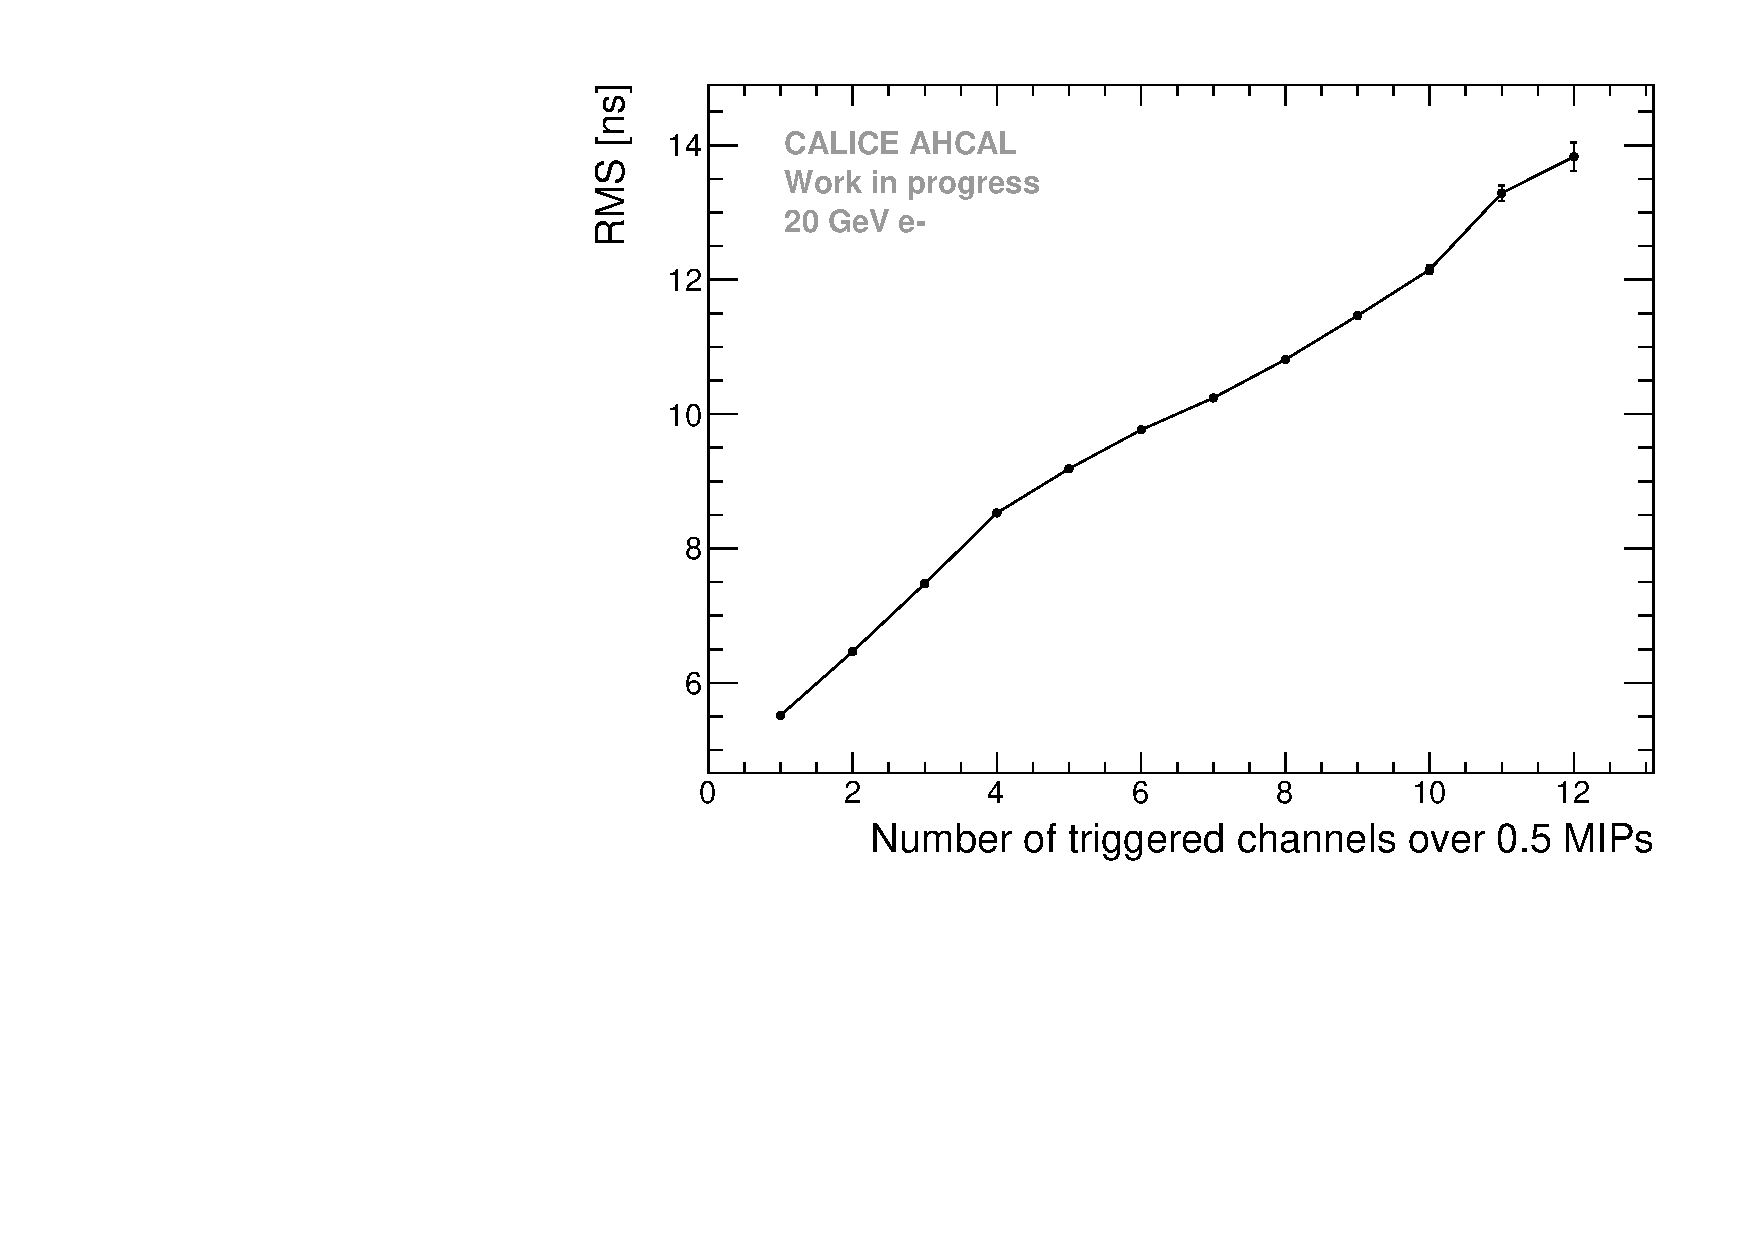
\includegraphics[width=1\textwidth]{chap5/fig_AHCAL_timing/Electrons/ParametrisationPedestalShift_20GeV.pdf}
		\caption{RMS of the time of first hit function of the number of triggered channels (20 GeV).}\label{fig:RMS_nHits}
	\end{subfigure}
	\caption{\subref{fig:nhits_profile} The fit region is between 1 and 15 hits. A linear dependence is clearly visible. \subref{fig:RMS_nHits} The RMS of the time distribution can increase up to 12 ns for a high number of triggered channels.}
\end{figure}

\subsection{Time of the first hit for electrons}
\label{subsec:Electron_Final}

\begin{figure}[htbp!]
	\begin{subfigure}[t]{0.45\textwidth}
		\centering
		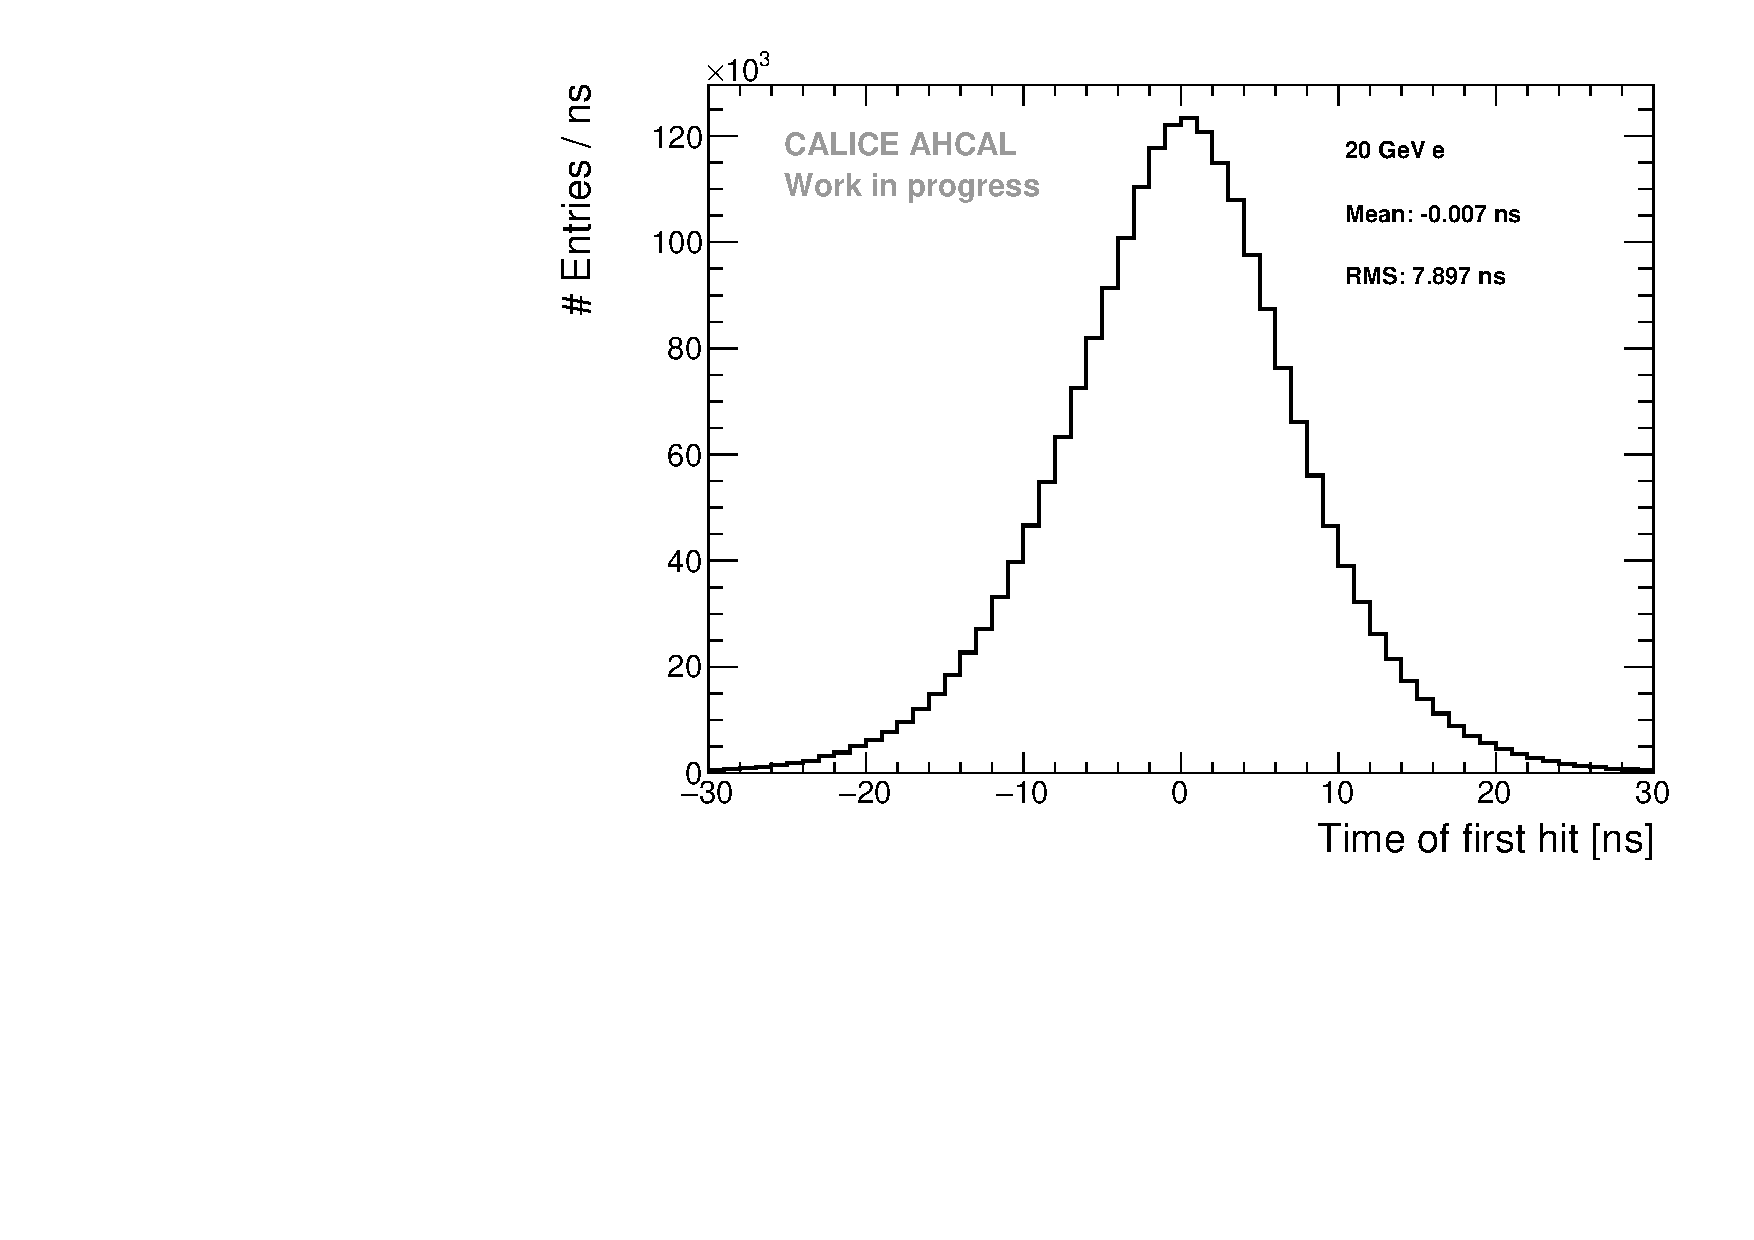
\includegraphics[width=1\textwidth]{chap5/fig_AHCAL_timing/Electrons/Timing_AllLayers_20GeV.pdf}
		\caption{Time of the first hit distribution for 20 GeV electrons after correction.}\label{fig:timing_electrons_corr}
	\end{subfigure}
	\hfill
	\begin{subfigure}[t]{0.45\textwidth}
		\centering
		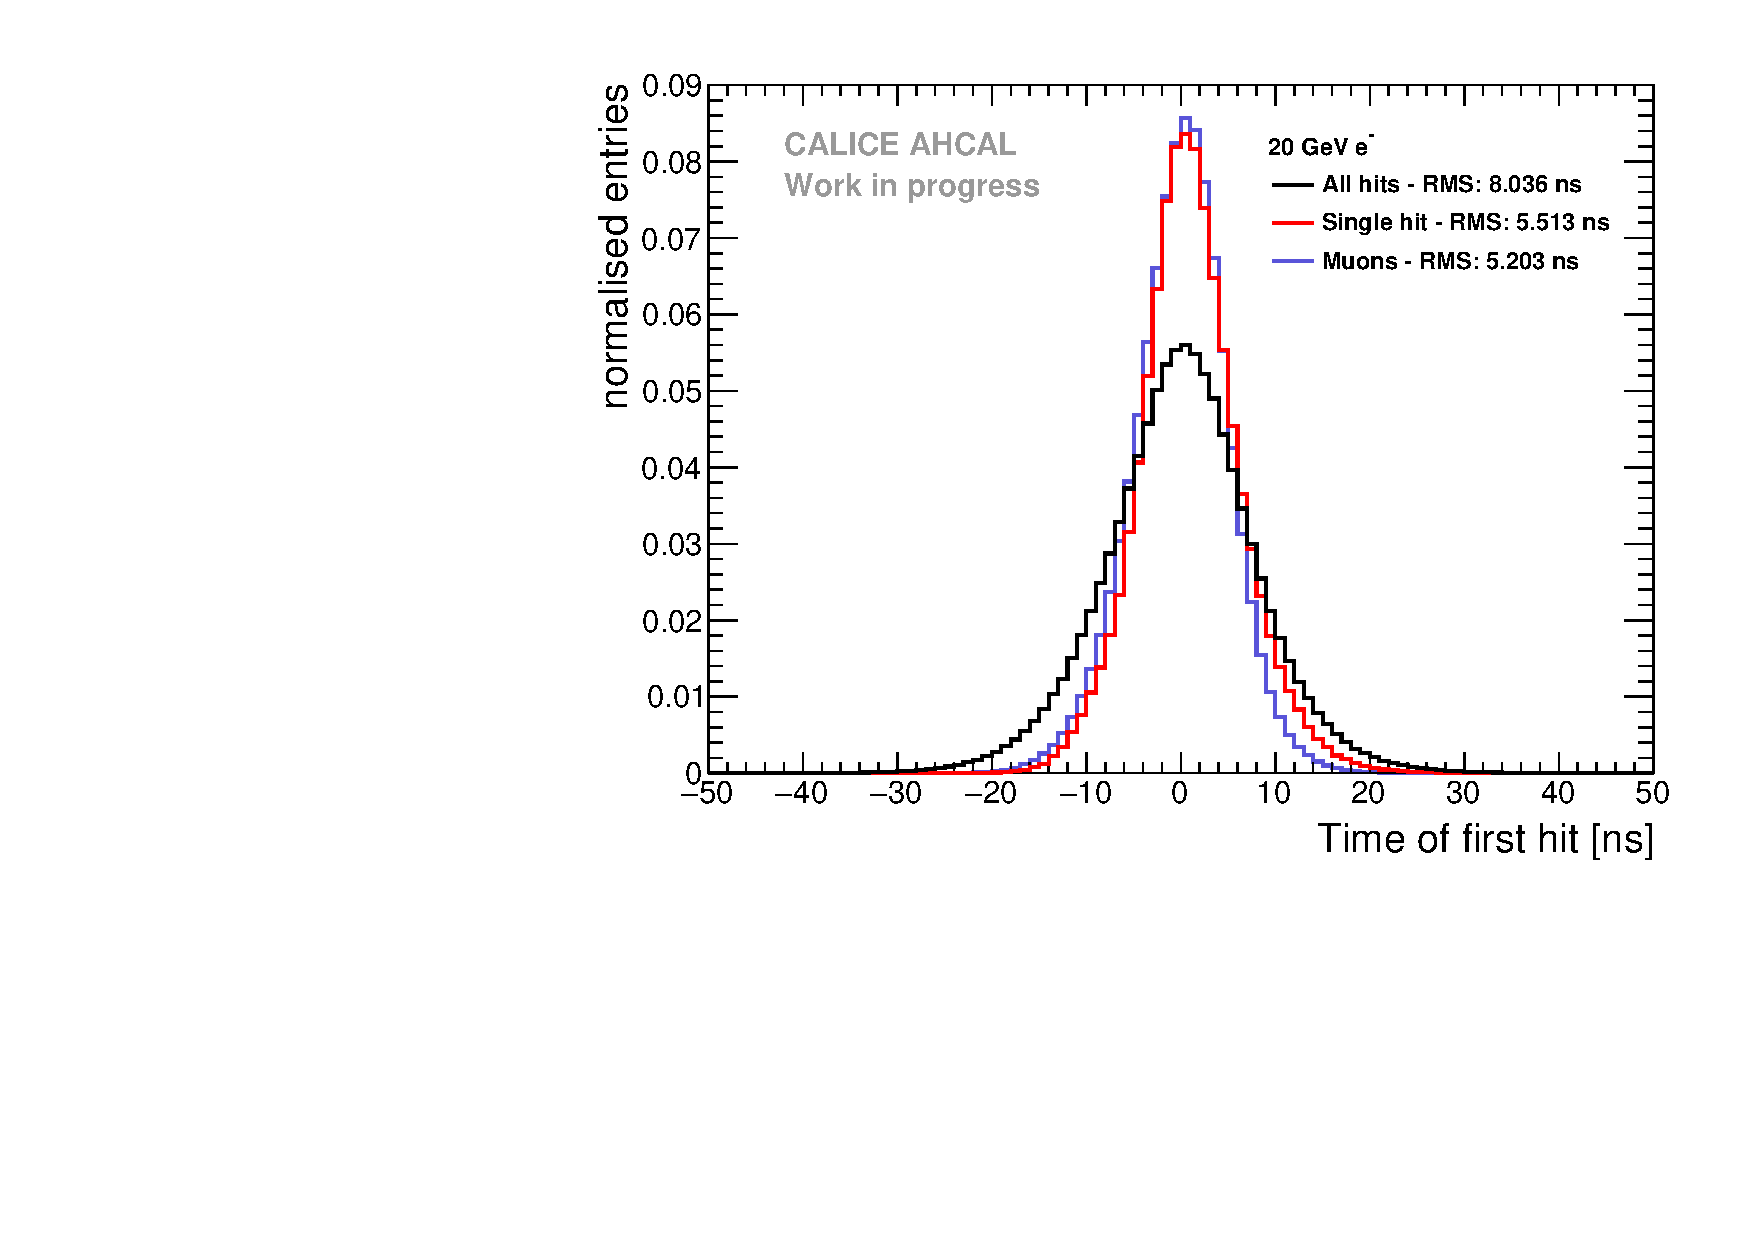
\includegraphics[width=1\textwidth]{chap5/fig_AHCAL_timing/Electrons/ComparisonAll_ElectronsSingleHit.pdf}
		\caption{Comparison with the muon time of first hit distribution.}\label{fig:timing_electron_muon_comp}
	\end{subfigure}
	\caption{\subref{fig:timing_electrons_corr} Time of the first hit distribution for 20 GeV electrons after number of triggered channel correction, $\mu$ = -0.005 ns, RMS = 7.62 ns. \subref{fig:timing_electron_muon_comp} Comparison of the electron data sample, the time distribution is very similar to the muon one if only events with single hits in a chip are taken.}
\end{figure}

The distribution of the time of the first for 20 GeV is shown in figure \ref{fig:timing_electrons_corr} after correction. As seen the correction improves the RMS of the distribution ($\sim$14.6\%) as well as the distribution appears more gaussian-like. However, there is still a discrepancy ($\sim$32.6\%) with the time resolution obtained for muons (5 ns). This is due to the fact that not only the mean time shifts but that the RMS also increases as a function of number of hits as seen in figure \ref{fig:RMS_nHits}. In order for the simulation to match the data, the increase of the width of the time distribution has to be parametrised from the data. More details can be read in the appendix \ref{appendix:ped_shift}. A comparison with the muon data has been done in order to cross-check the calibration as seen in figure \ref{fig:timing_electron_muon_comp}. If only single hits in a chip are taken, the time resolution obtained is very similar to the time resolution observed in muons ($\sim$7.7\% difference).\\
The cause of observed effect is most likely due to an element in the chip (a delay box) that get unstable with the number of triggered channels and that is responsible for the hold of the TDC value in the chip. The hold is delayed thus sampling a higher TDC value than the one expected. All electron runs have been checked to validate the correction and calibration procedure. The figure \ref{fig:all_electron_energies} shows the comparison from 10 GeV to 50 GeV. The distributions are in agreement within a 10-15\% range for all energies which is within systematical uncertainty as explained in subsection \ref{subsec:det_inhomo}.

\begin{figure}[htbp!]
	\centering
	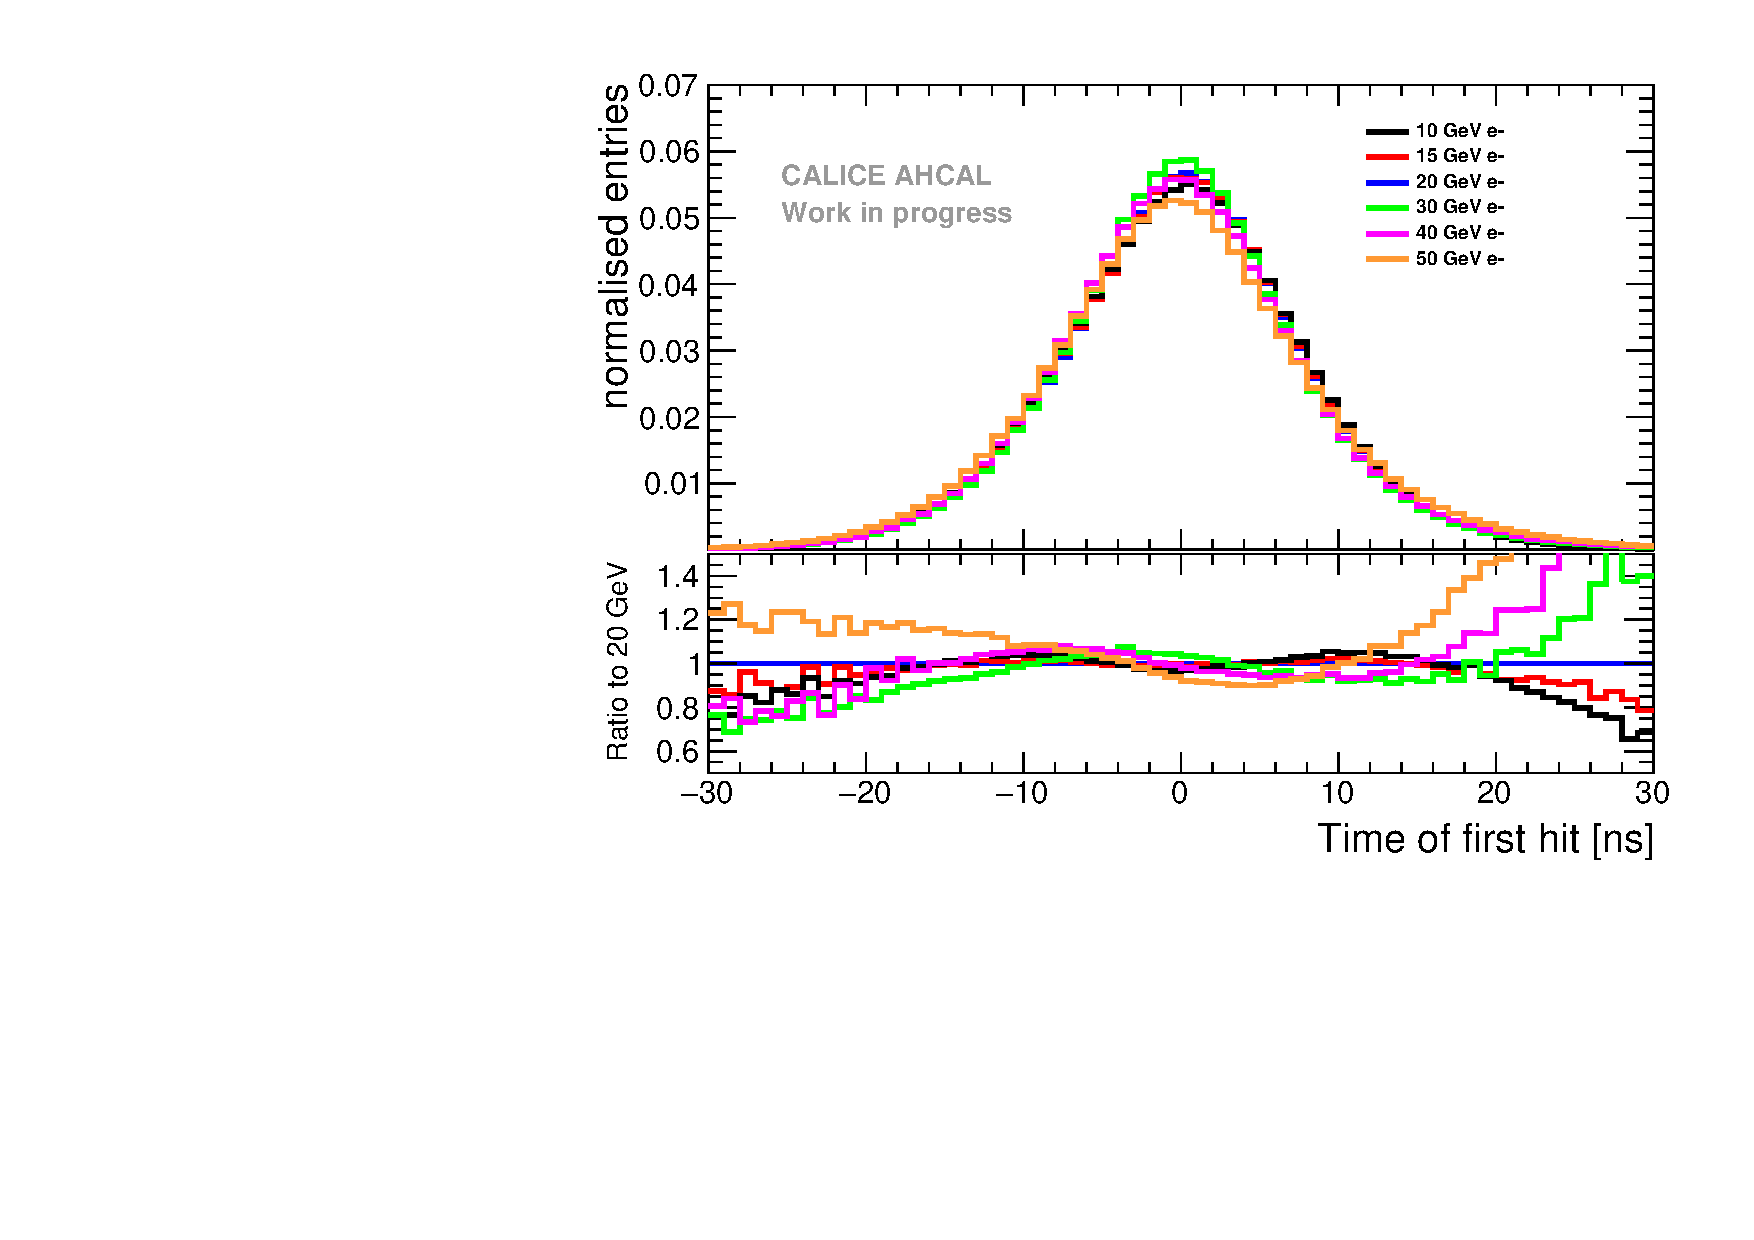
\includegraphics[width=1\textwidth]{chap5/fig_AHCAL_timing/Electrons/ComparisonDataEnergies.pdf}
	\caption{Comparison of the time of first hit distribution for all electron energies.}
	\label{fig:all_electron_energies}
\end{figure}

\subsection{Influence of the detector inhomogeneity}
\label{subsec:det_inhomo}

A study has been performed to estimate the influence of the detector inhomogeneity on timing independent of the beam profile. For this, only events in which the centre of gravity in x and y are within the 4 centre tiles of the detector are selected. This has been checked for 10 and 50 GeV electron beam energy. The difference between the distribution can help to estimate the systematic uncertainty due to the inhomogeneity of the detector.
\begin{figure}[htbp!]
	\begin{subfigure}[t]{0.45\textwidth}
		\centering
		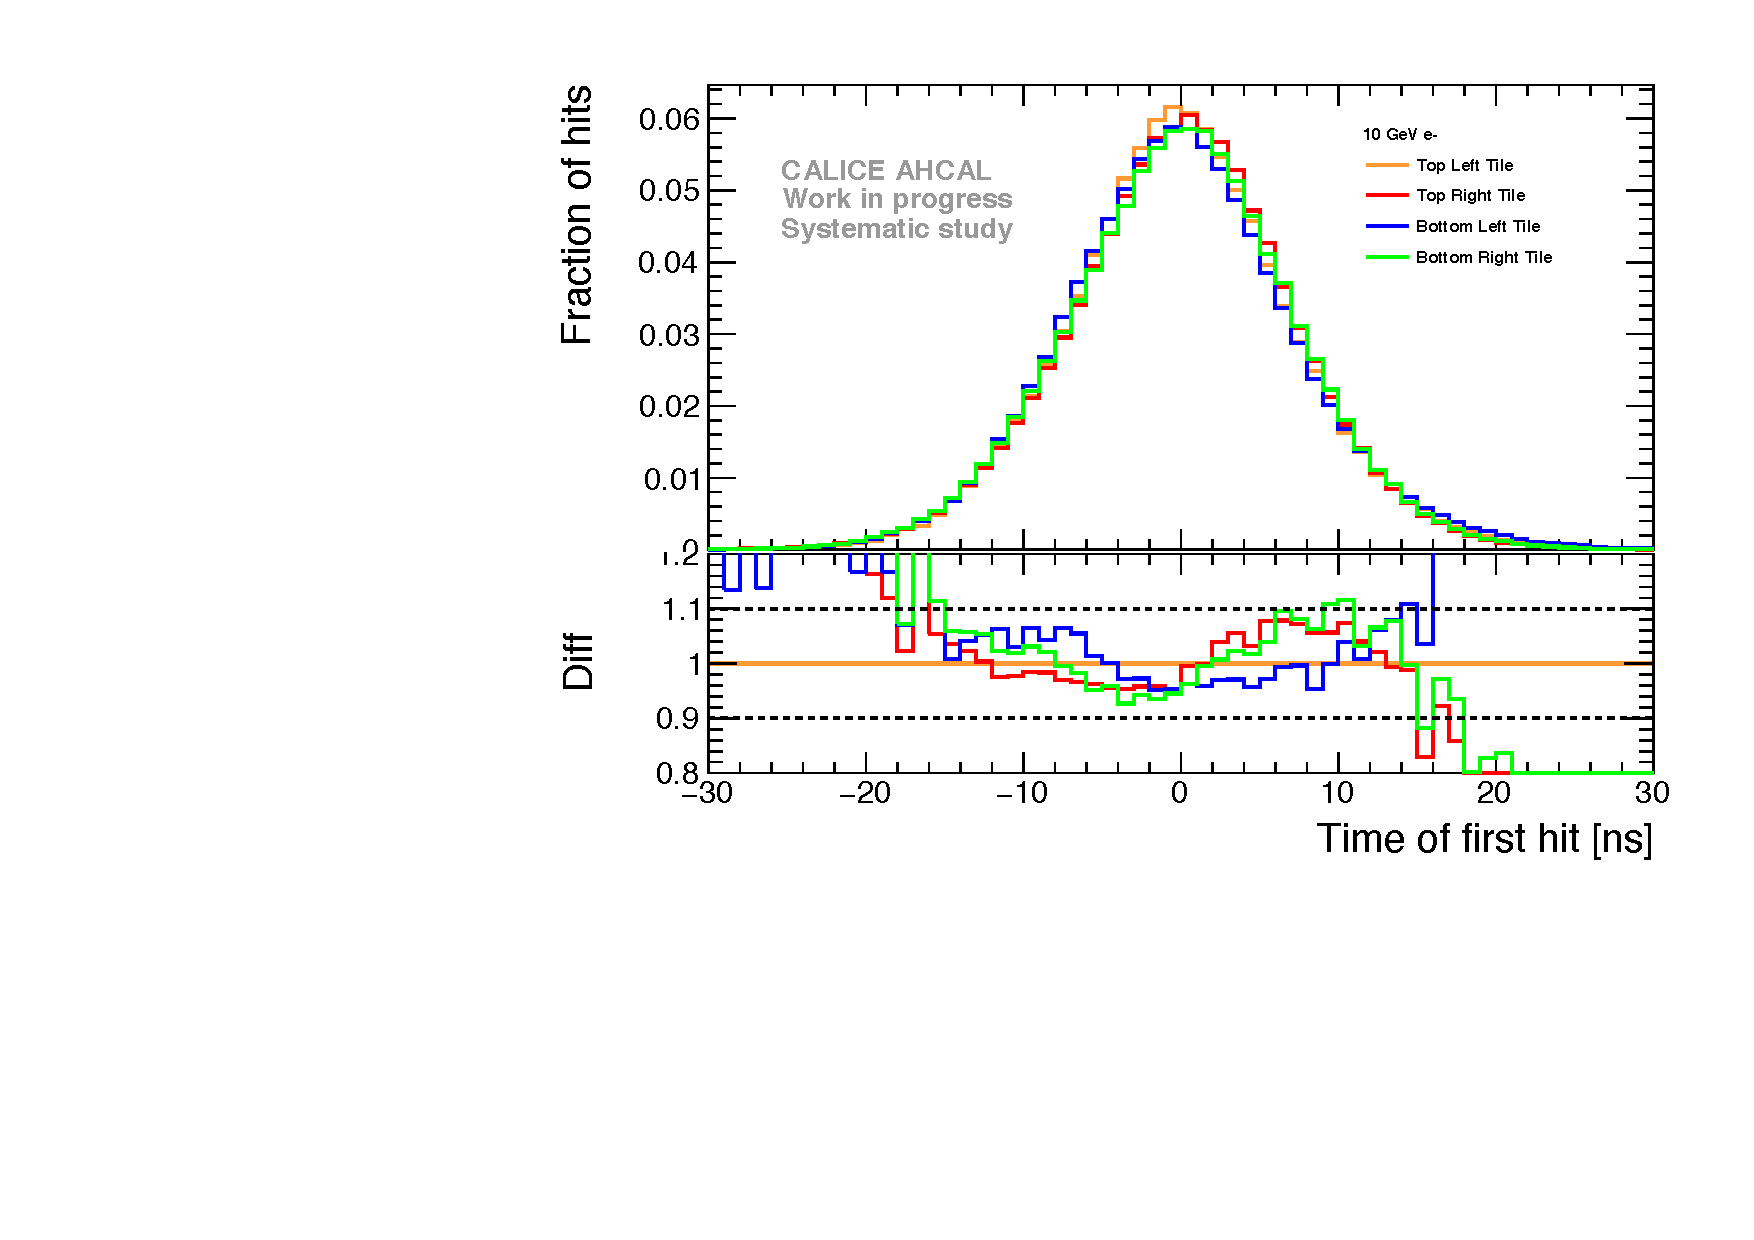
\includegraphics[width=1\textwidth]{chap5/fig_AHCAL_timing/Electrons/Systematic_Inhomogeneity_10GeV.pdf}
		\caption{Time of the first hit distribution at 10 GeV.}\label{fig:timing_inhomo_10GeV}
	\end{subfigure}
	\hfill
	\begin{subfigure}[t]{0.45\textwidth}
		\centering
		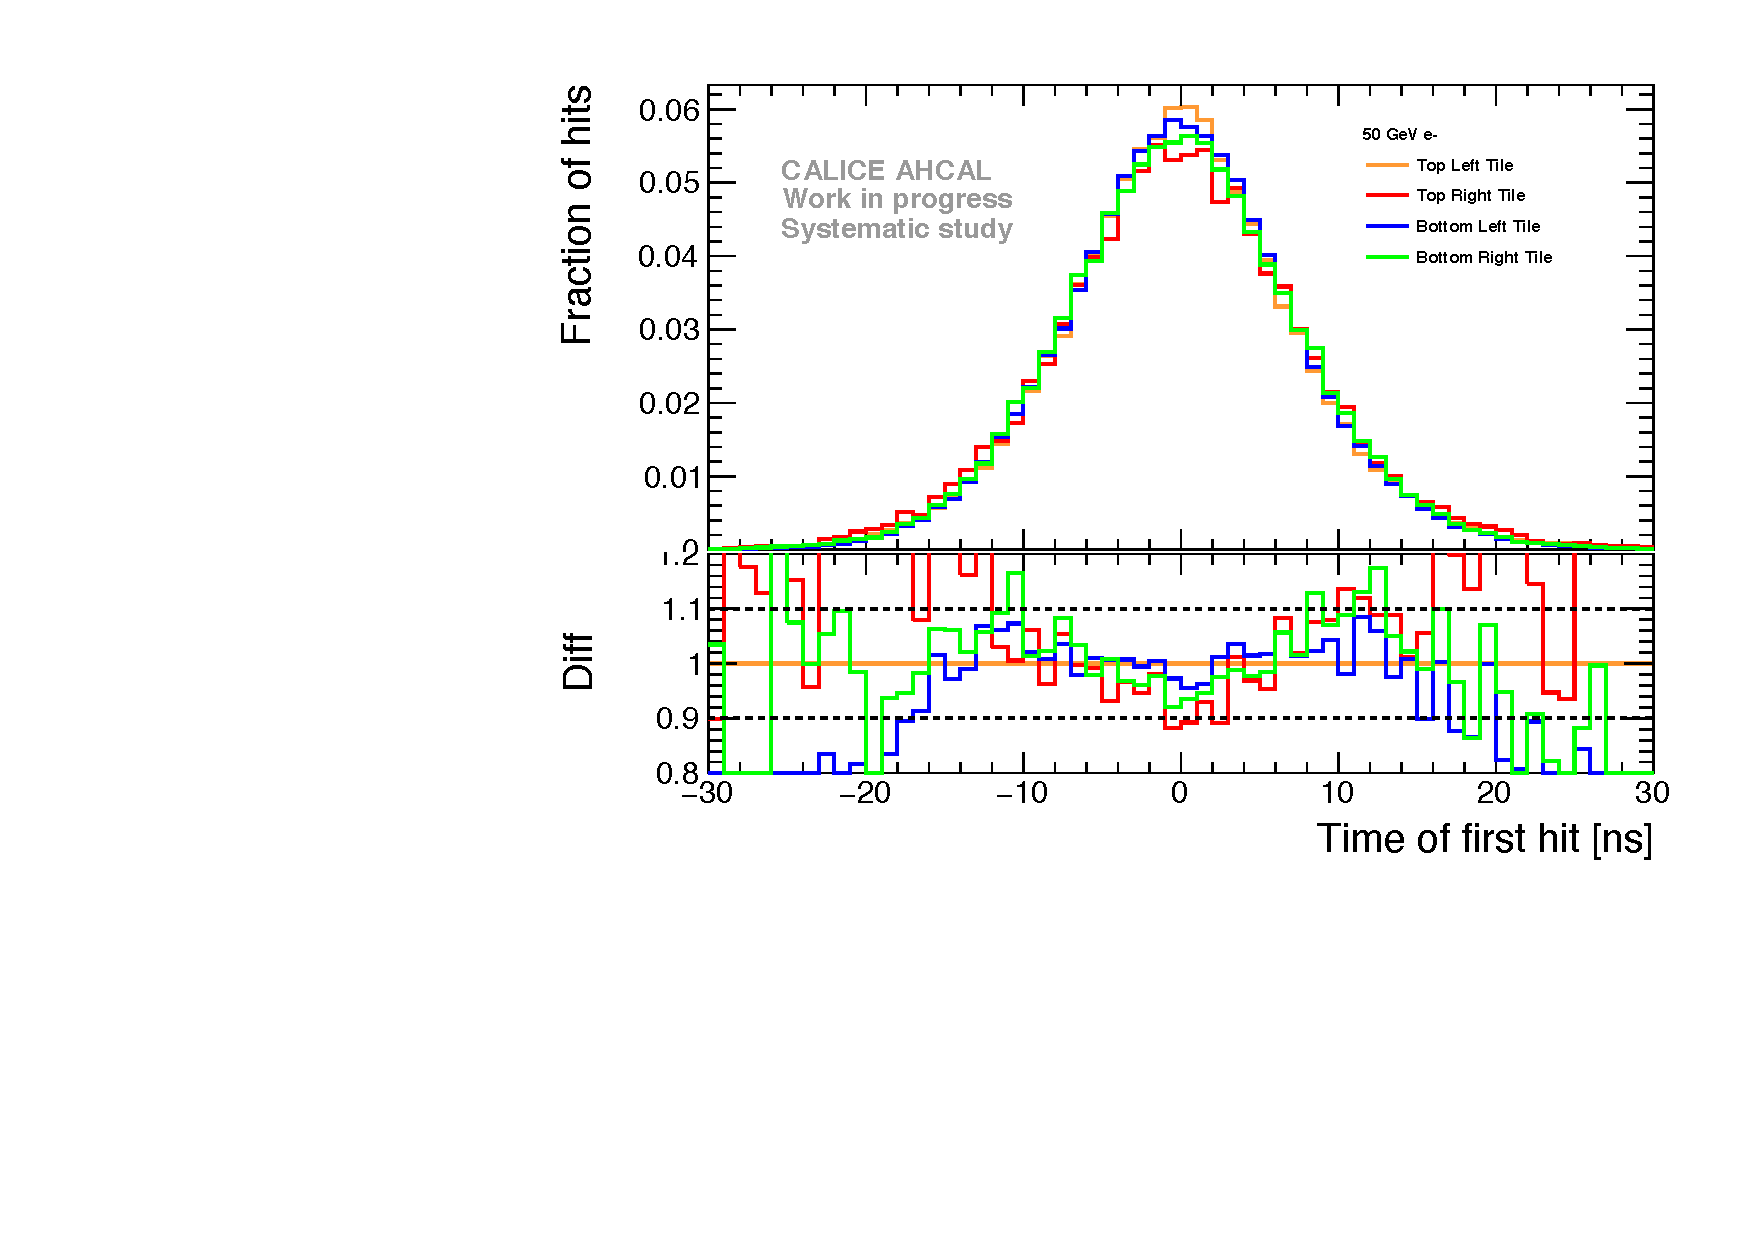
\includegraphics[width=1\textwidth]{chap5/fig_AHCAL_timing/Electrons/Systematic_Inhomogeneity_50GeV.pdf}
		\caption{Time of the first hit distribution at 50 GeV.}\label{fig:timing_inhomo_50GeV}
	\end{subfigure}
	\caption{\subref{fig:timing_inhomo_10GeV} Time of the first hit distribution for all 4 tiles at 10 GeV. All distribution are within 10-15\% in the core. \subref{fig:timing_inhomo_50GeV} Time of the first hit distribution for all 4 tiles at 50 GeV. All distribution are within 10-15\% in the core.}
\end{figure}
The figures \ref{fig:timing_inhomo_10GeV} and \ref{fig:timing_inhomo_50GeV} show the time distribution for each tiles at 10 and 50 GeV respectively. The ratio shown is compared to the top left centre tile. One can see that for both energies, the distributions are within a 10-15\% agreement. Therefore a conservative systematic uncertainty of 15\% is assigned to electron and pion data in the following.

\section{Comparison with simulation for muons and electrons}

The next step is to compare data with simulation and cross-check the simulation with electrons. The timing resolution is extracted from muon data runs by fitting a double Gaussian in the range [-50 ns, 50 ns] and is used to smear the timing of simulated hits. The table \ref{table:time_res_sim} sums up the parameters used. The comparison for muons is shown in figure \ref{fig:sim_data_muon}. The comparison shows that in the full range, the difference between data and simulation is around 10-20\% maximum. This may be because of the asymmetry present in data that might be not well reproduced in Monte-Carlo. In general, the simulation is in a good agreement with data.

\begin{table}[htb!]
	\centering
	\caption[Timing resolution extracted with a double Gaussian fit from muon data used for simulation.]{Timing resolution extracted with a double Gaussian fit from muon data used for simulation.\footnotemark[1]}
	\label{table:time_res_sim}
	\begin{tabular}{@{} cccc @{}}
		\hline
		$\mu_{1}$ [ns] & $\sigma_{1}$ [ns] & $\mu_{2}$ [ns] & $\sigma_{2}$ [ns] \\
		\hline
		-0.699095 & 5.8589 & 0.945278 & 3.40119 \\
		\hline
	\end{tabular}
\end{table}
\footnotetext{A table of rejected chips is available in appendix \ref{appendix:rejection}.}

\begin{figure}[htbp!]
	\centering
	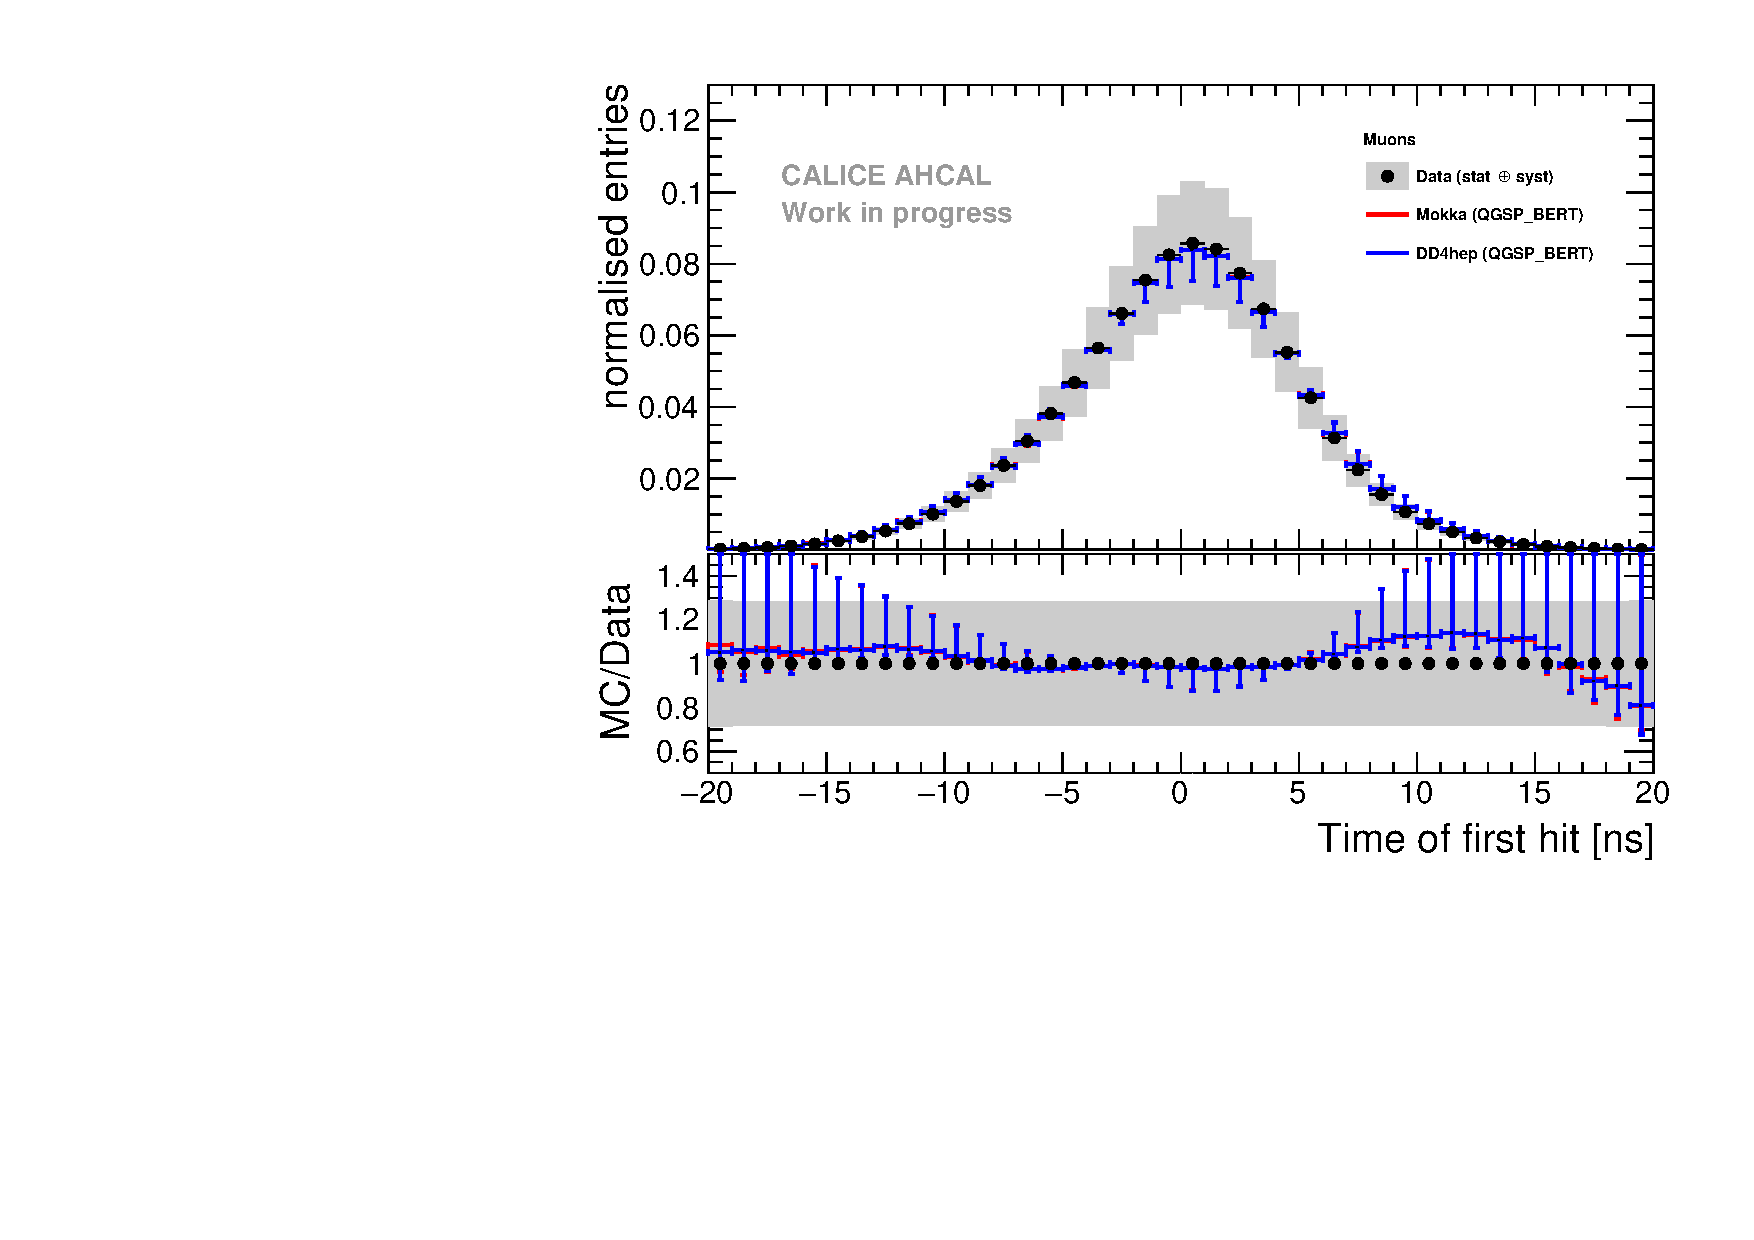
\includegraphics[width=0.6\textwidth]{chap5/fig_AHCAL_timing/Muons/Comparison_MokkaDD4hepData_Muons.pdf}
	\caption{Time of first hit for data and simulation between -20 and 20 ns.}
	\label{fig:sim_data_muon}
\end{figure}

In the next step, a comparison with electron data is necessary to validate the simulation. In addition to the muon resolution, a parametrisation of the increase of the width of the time distribution function of the number of hits above 0.5 MIPs is added in simulation as described in appendix \ref{appendix:ped_shift}. The figure \ref{fig:sim_data_elec} shows this comparison. The simulation is systematically narrower than data for all energies. This would suggest that simulation has less hits than data which is in agreement with figure \ref{fig:sim_data_elec_nHits}, where generally simulation is 10-20\% lower than data in the region of interest of 6 to 10 hits per chip. The simulation is in better agreement for higher energies (40-50 GeV) than for lower energies (10-15 GeV). This might come from the inhomogeneity of the detector that is not well reproduced in simulation by the global time parametrisation used. This may suggest that the time parametrisation is chip-wise of layer-wise. But due to the limited amount of data, only a global time parametrisation can be applied. For 10 to 20 GeV comparisons, the description of the tails in simulation are quite underestimated. This may be due to the description of the noise in simulation that is not perfectly reproduced. Overall, the simulation and data are in agreement within uncertainties.

\begin{figure}[htbp!]
	\begin{subfigure}[t]{0.45\textwidth}
		\centering
		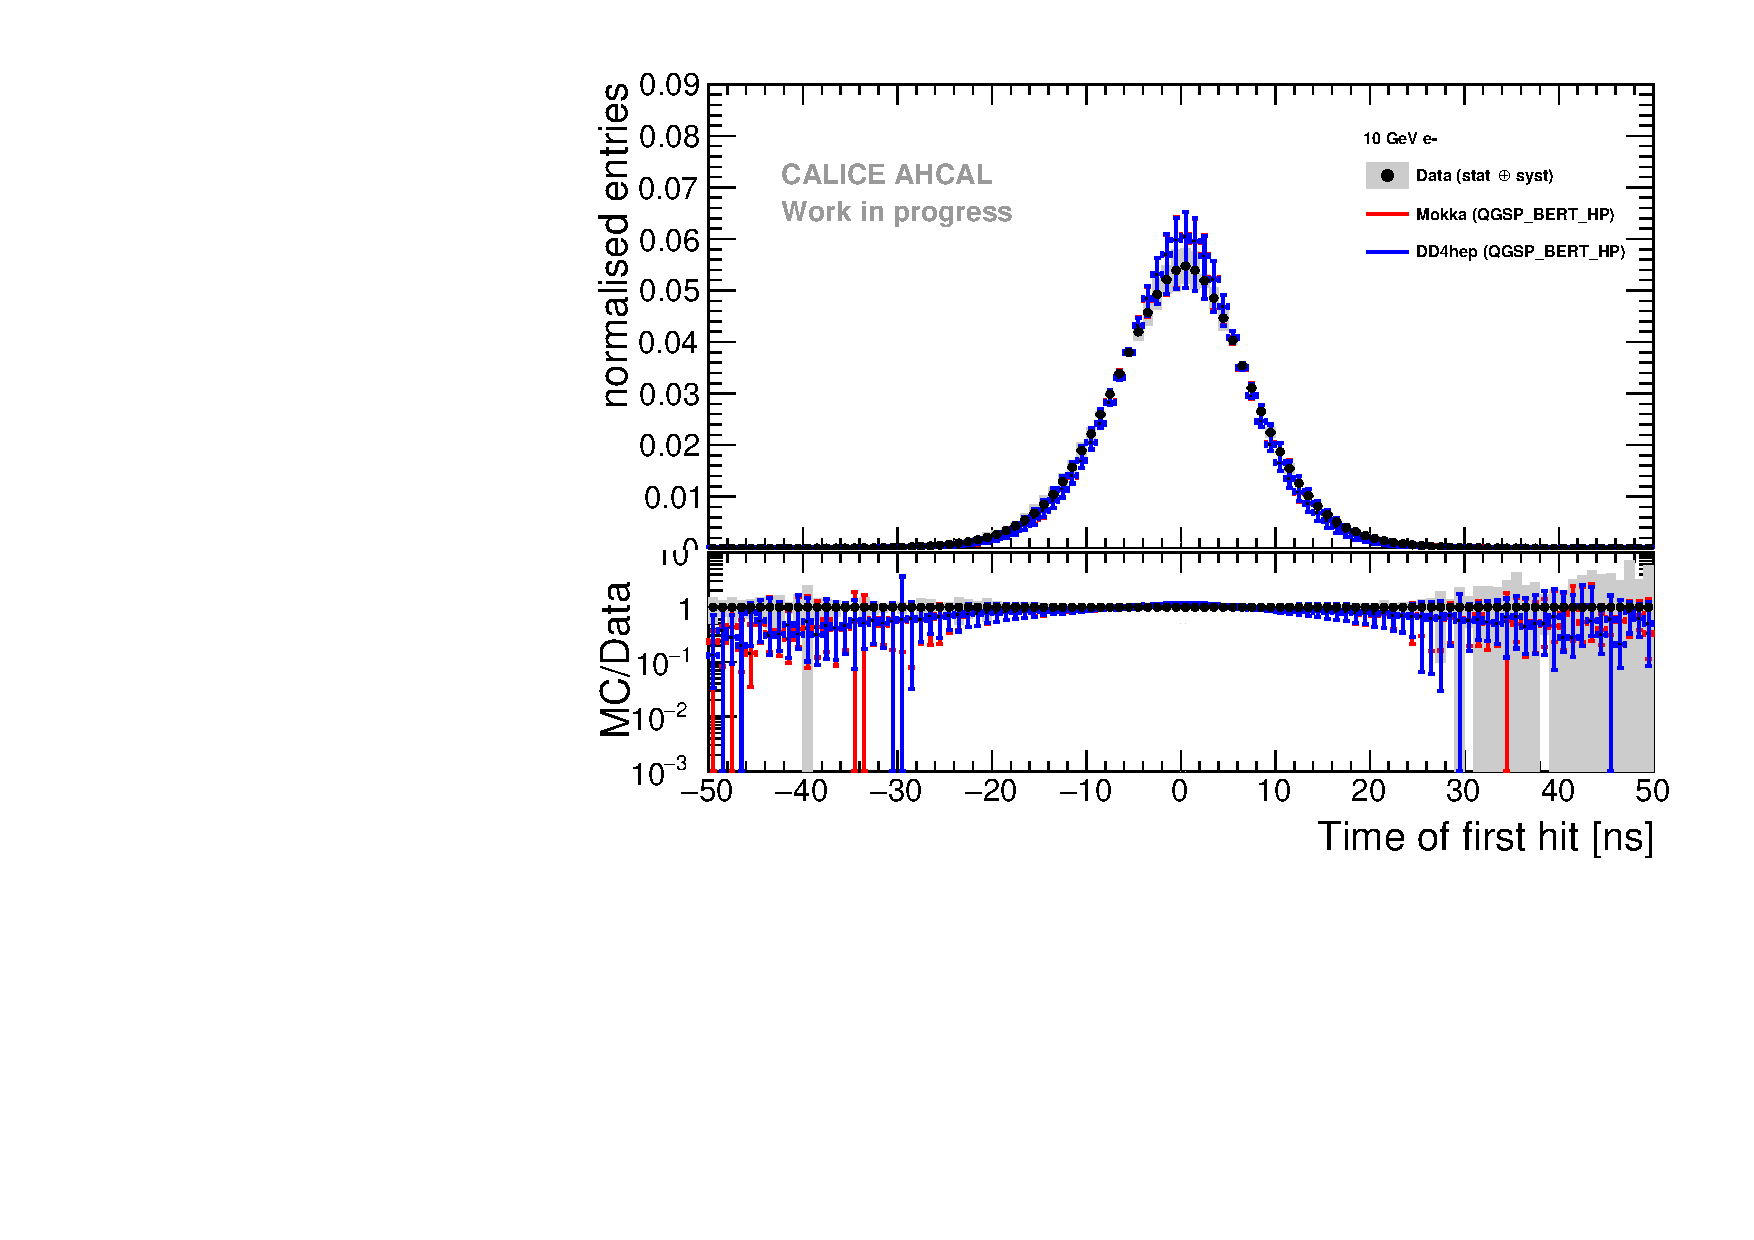
\includegraphics[width=1\textwidth]{chap5/fig_AHCAL_timing/Electrons/Comparison_SimData_Electrons10GeV.pdf}
		\caption{10 GeV.}\label{fig:elec_sim_data_10GeV}
	\end{subfigure}
	\hfill
	\begin{subfigure}[t]{0.45\textwidth}
		\centering
		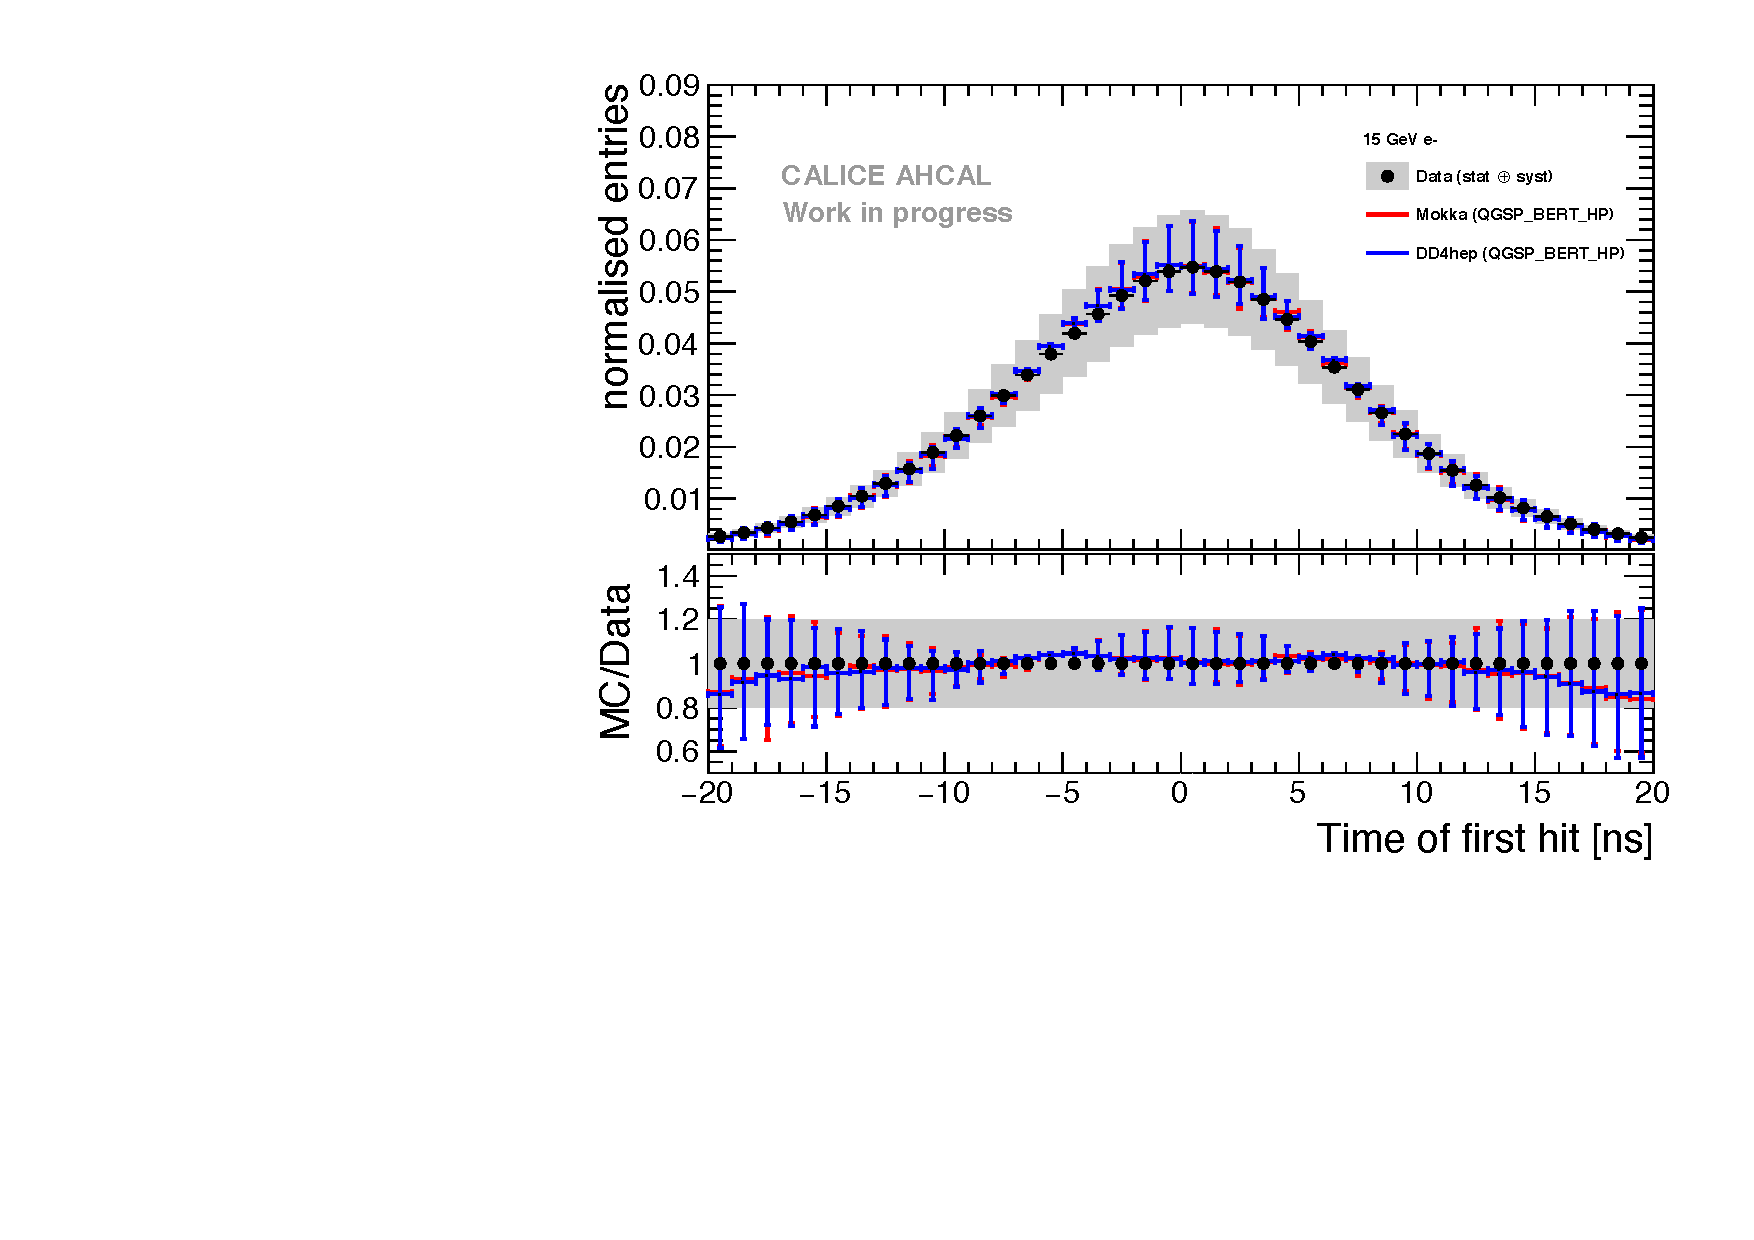
\includegraphics[width=1\textwidth]{chap5/fig_AHCAL_timing/Electrons/Comparison_SimData_Electrons15GeV.pdf}
		\caption{15 GeV.}\label{fig:elec_sim_data_15GeV}
	\end{subfigure}
	\hfill
	\begin{subfigure}[t]{0.45\textwidth}
		\centering
		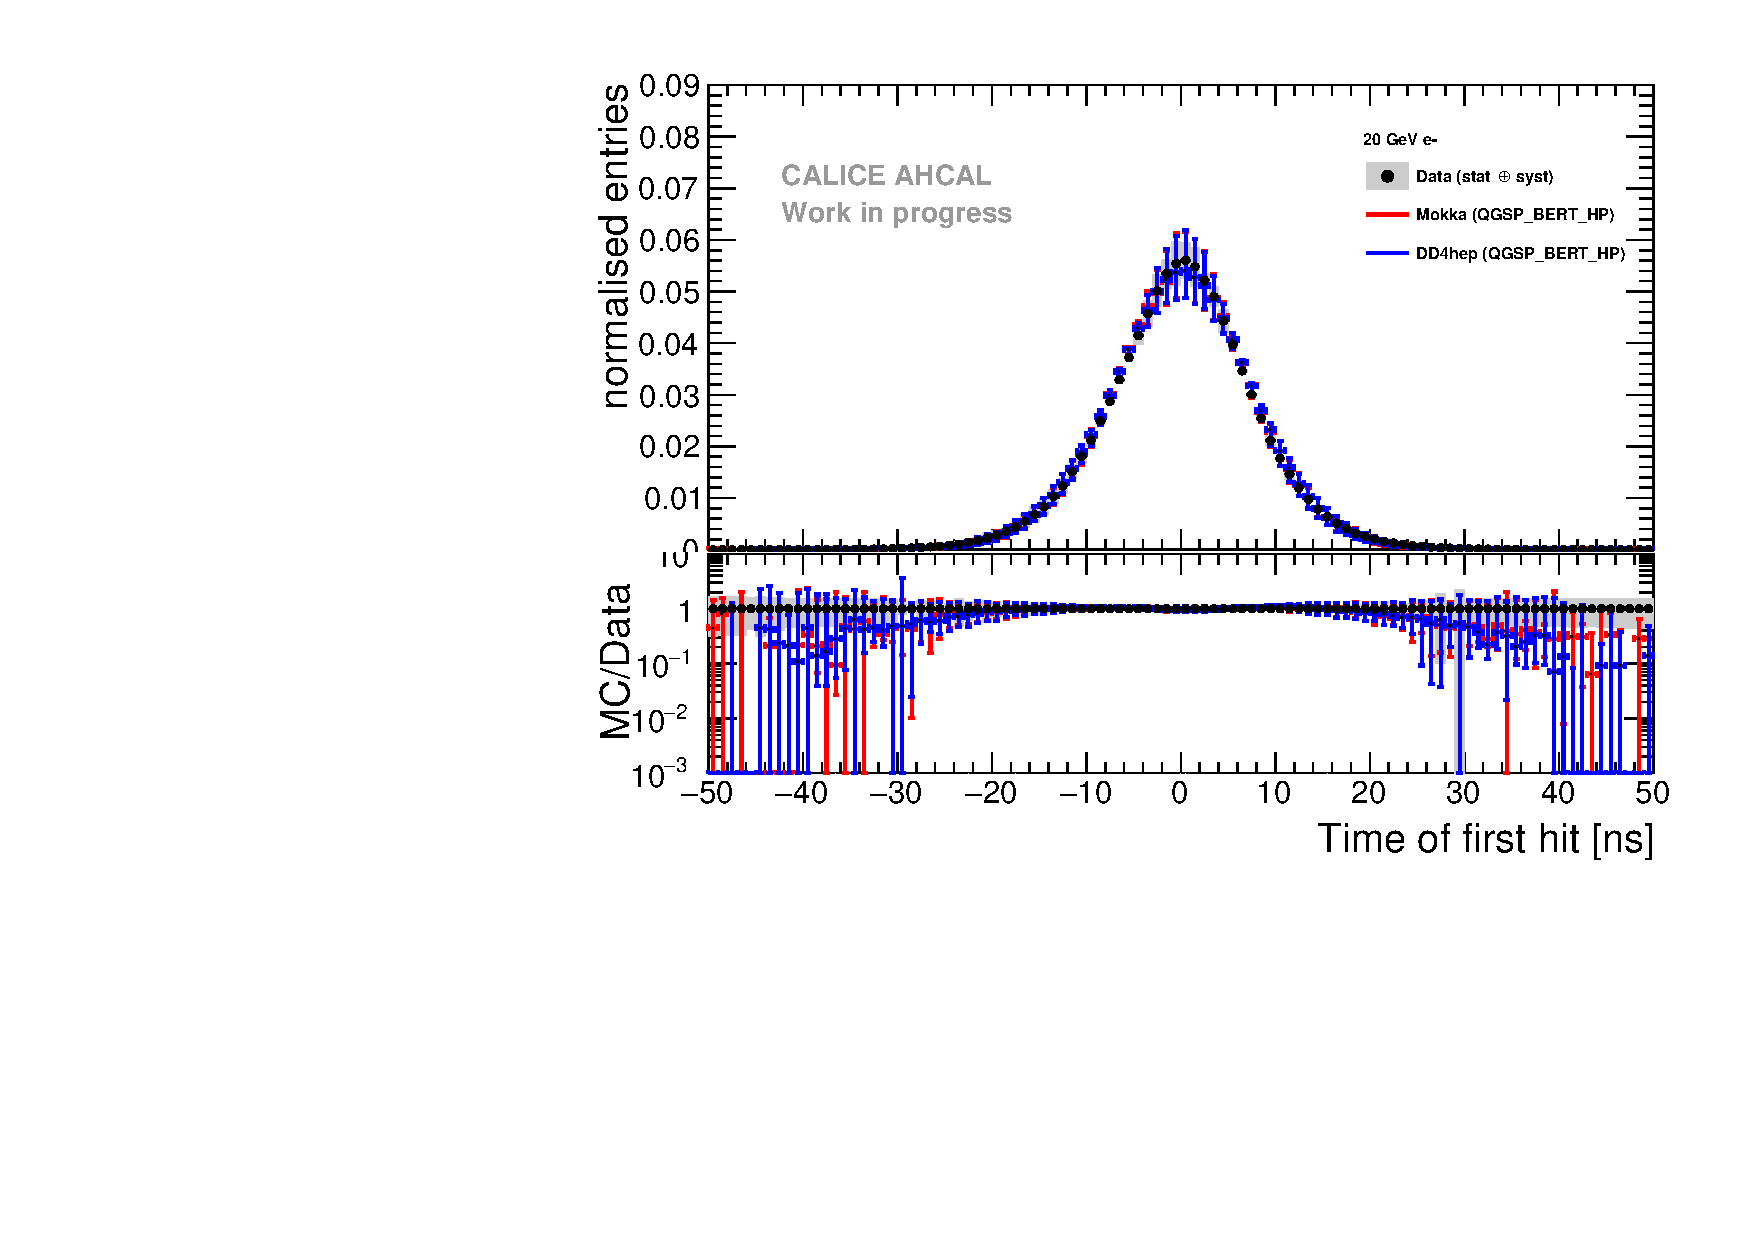
\includegraphics[width=1\textwidth]{chap5/fig_AHCAL_timing/Electrons/Comparison_SimData_Electrons20GeV.pdf}
		\caption{20 GeV.}\label{fig:elec_sim_data_20GeV}
	\end{subfigure}
	\hfill
	\begin{subfigure}[t]{0.45\textwidth}
		\centering
		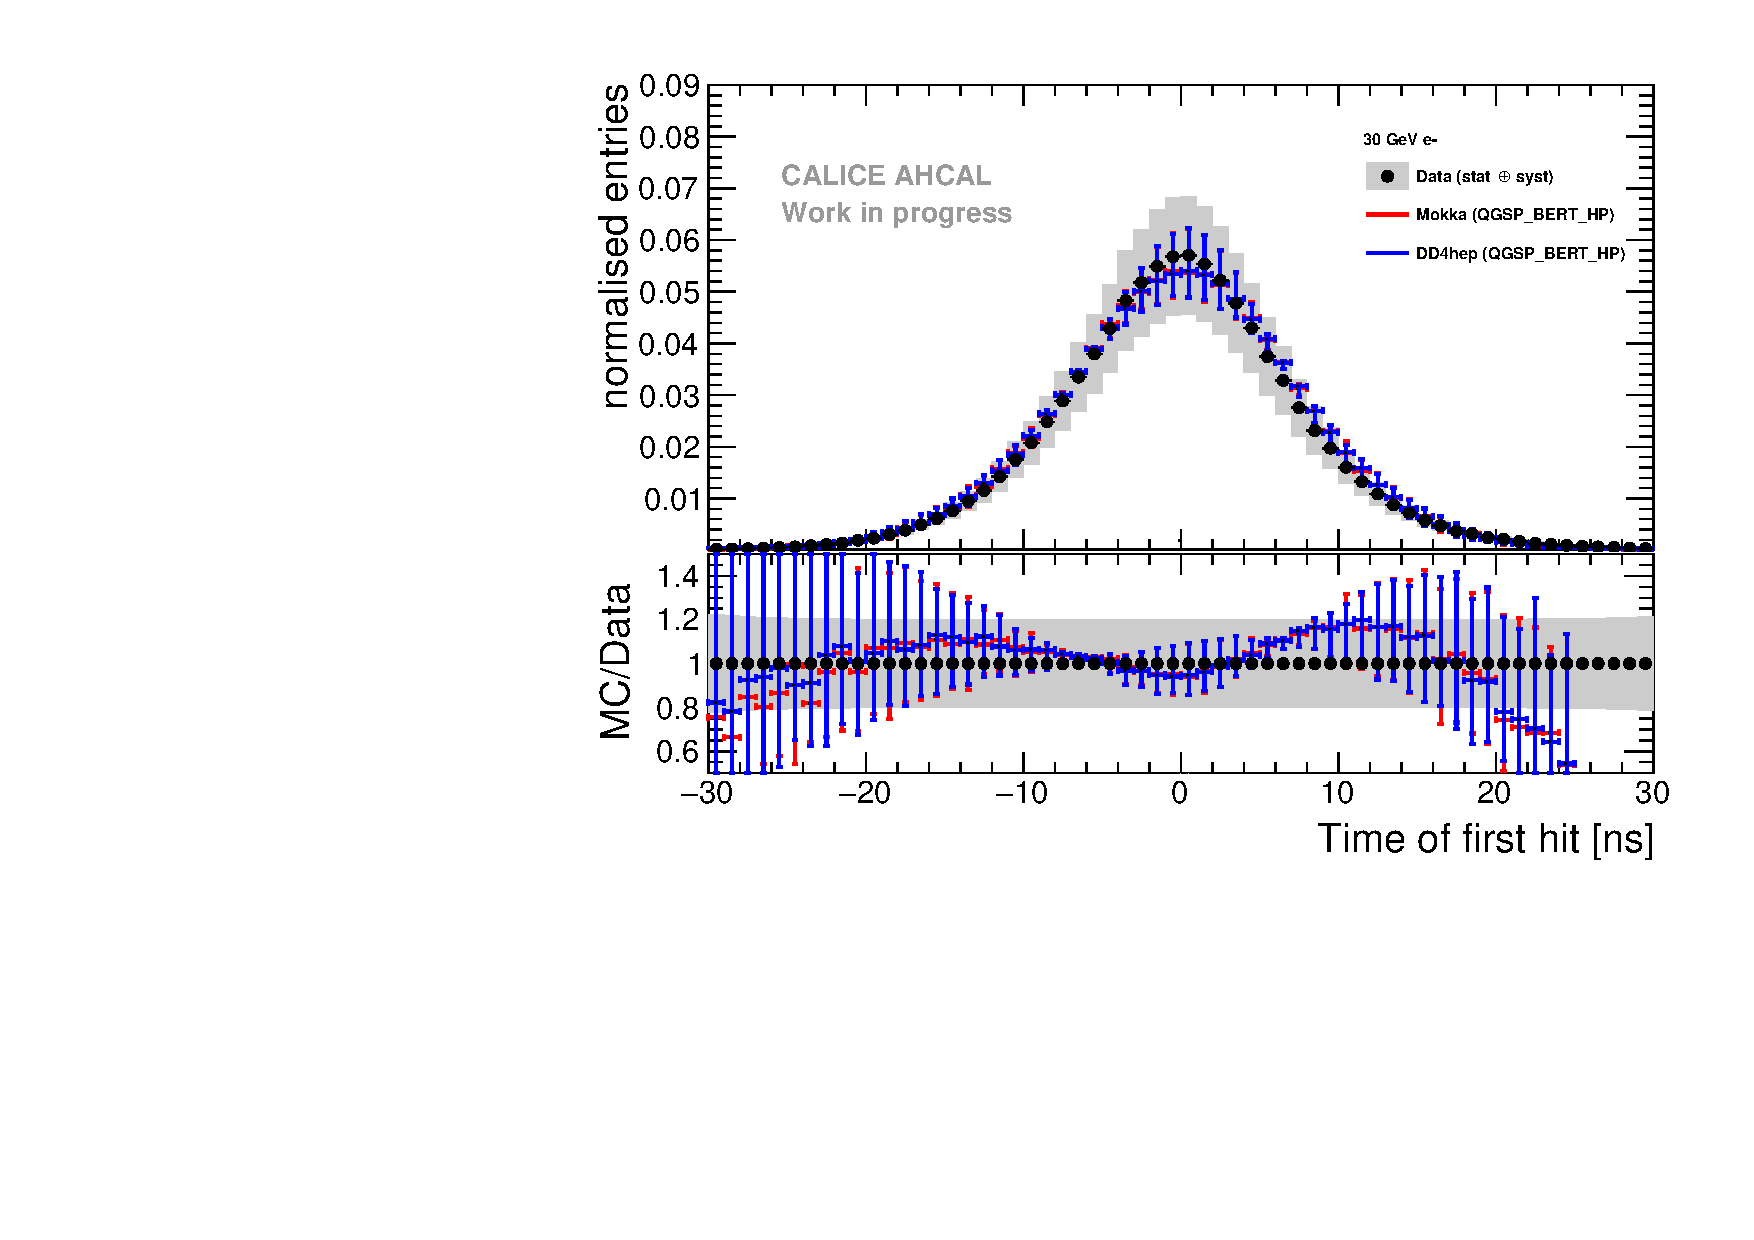
\includegraphics[width=1\textwidth]{chap5/fig_AHCAL_timing/Electrons/Comparison_SimData_Electrons30GeV.pdf}
		\caption{30 GeV.}\label{fig:elec_sim_data_30GeV}
	\end{subfigure}
	\hfill
	\begin{subfigure}[t]{0.45\textwidth}
		\centering
		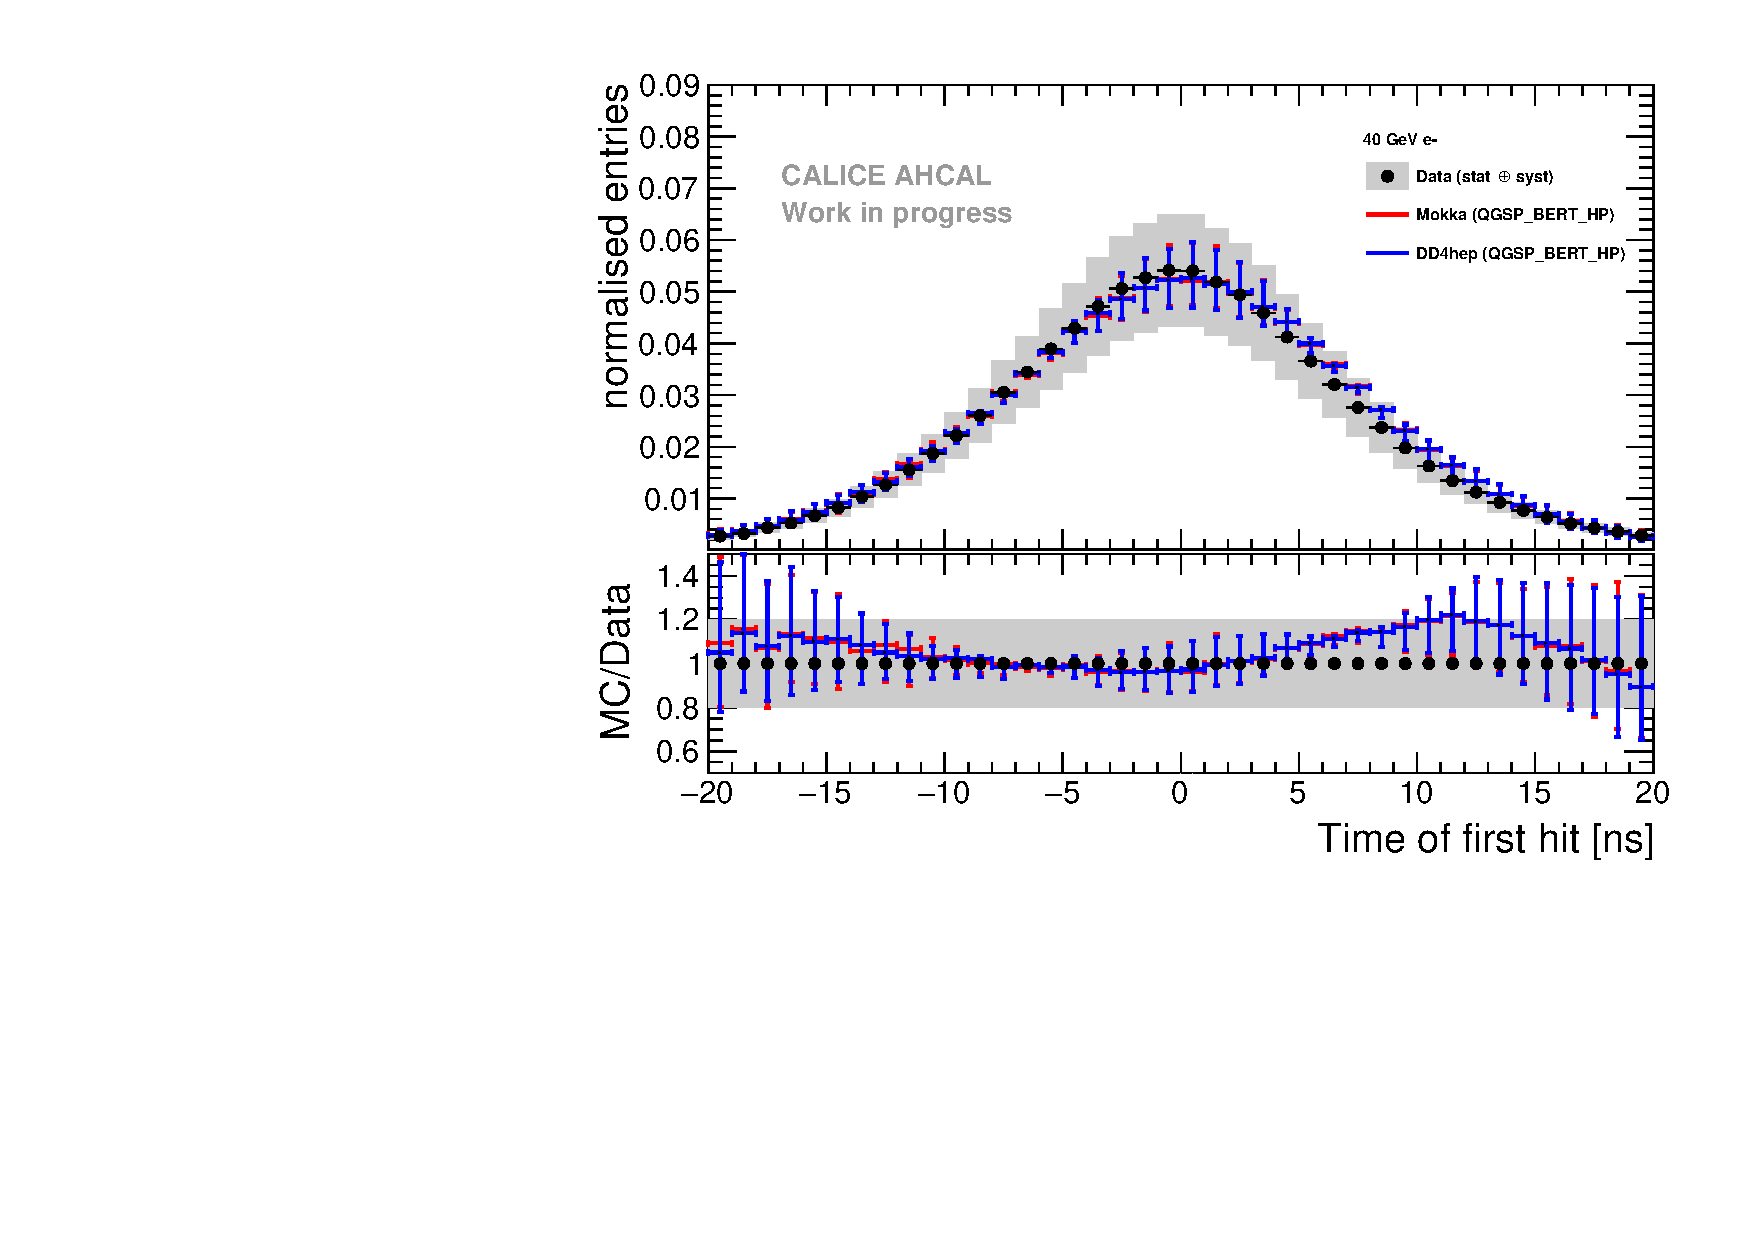
\includegraphics[width=1\textwidth]{chap5/fig_AHCAL_timing/Electrons/Comparison_SimData_Electrons40GeV.pdf}
		\caption{40 GeV.}\label{fig:elec_sim_data_40GeV}
	\end{subfigure}
	\hfill
	\begin{subfigure}[t]{0.45\textwidth}
		\centering
		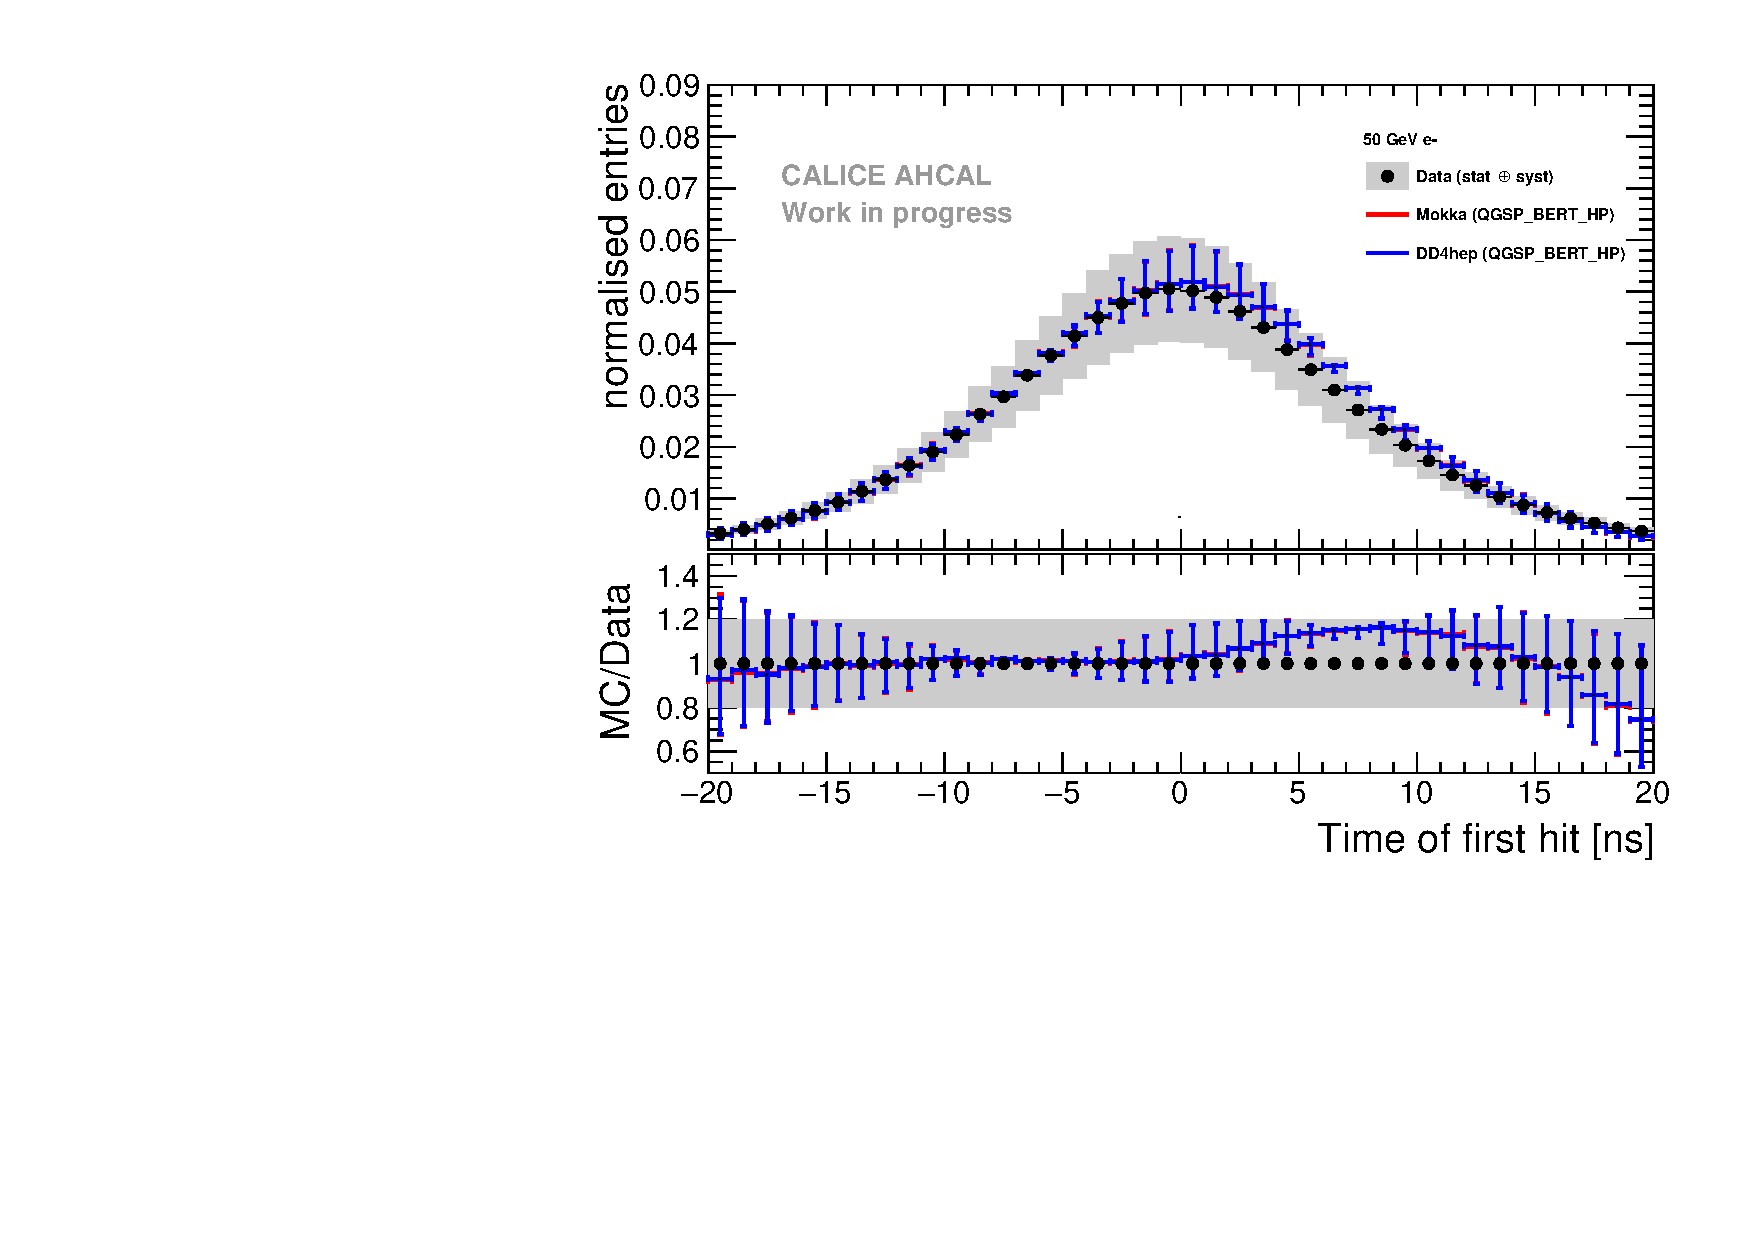
\includegraphics[width=1\textwidth]{chap5/fig_AHCAL_timing/Electrons/Comparison_SimData_Electrons50GeV.pdf}
		\caption{50 GeV.}\label{fig:elec_sim_data_50GeV}
	\end{subfigure}
	\caption{Comparison between electron data and MC for all energies of the time of first hit. The grey area represents the statistical and systematical error of the data. Error bars in simulation are obtained by varying the cross-talk parameter and with the error envelope from the number of hits parameterisation.}
	\label{fig:sim_data_elec}
\end{figure}

\begin{figure}[htbp!]
	\begin{subfigure}[t]{0.45\textwidth}
		\centering
		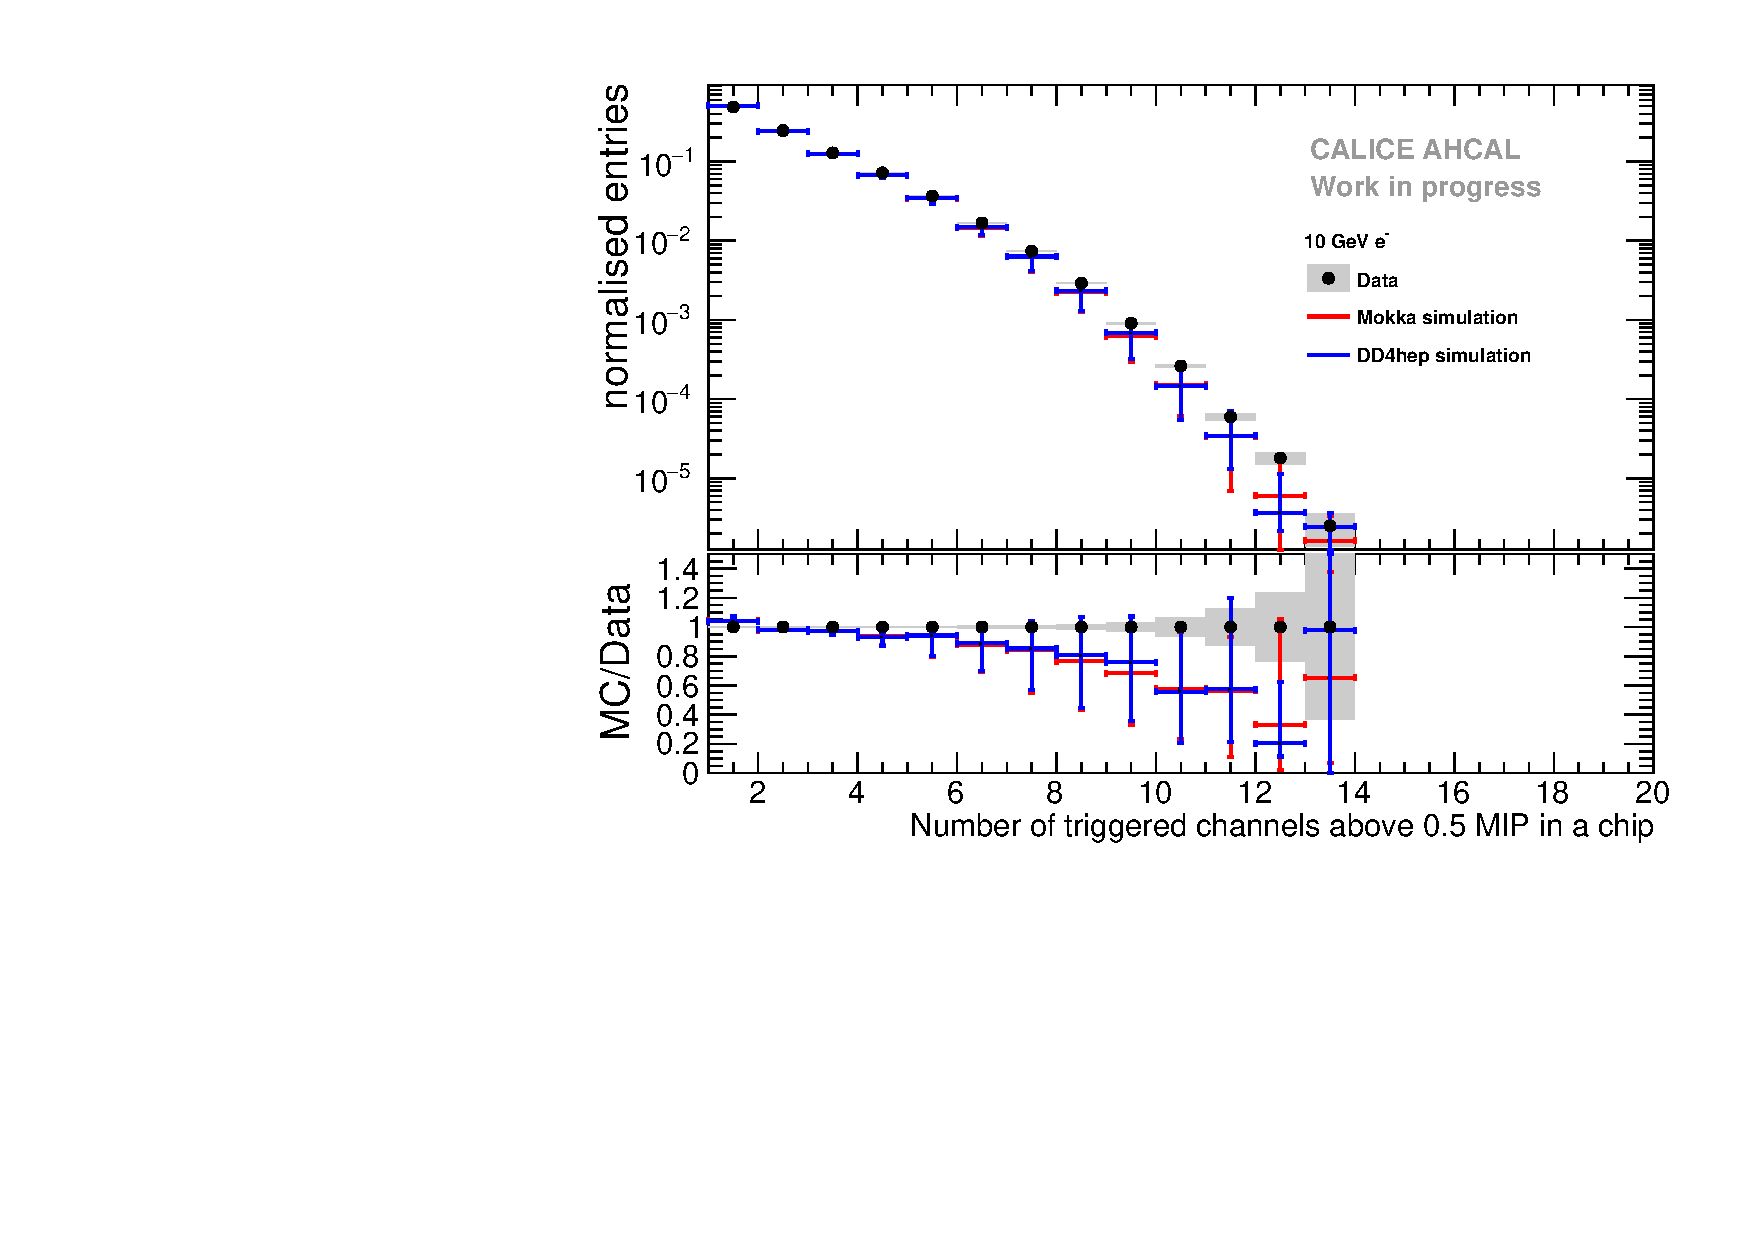
\includegraphics[width=1\textwidth]{chap5/fig_AHCAL_timing/Electrons/Comparison_SimData_Electrons_nHits_10GeV.pdf}
		\caption{10 GeV.}\label{fig:elec_sim_data_nHits_10GeV}
	\end{subfigure}
	\hfill
	\begin{subfigure}[t]{0.45\textwidth}
		\centering
		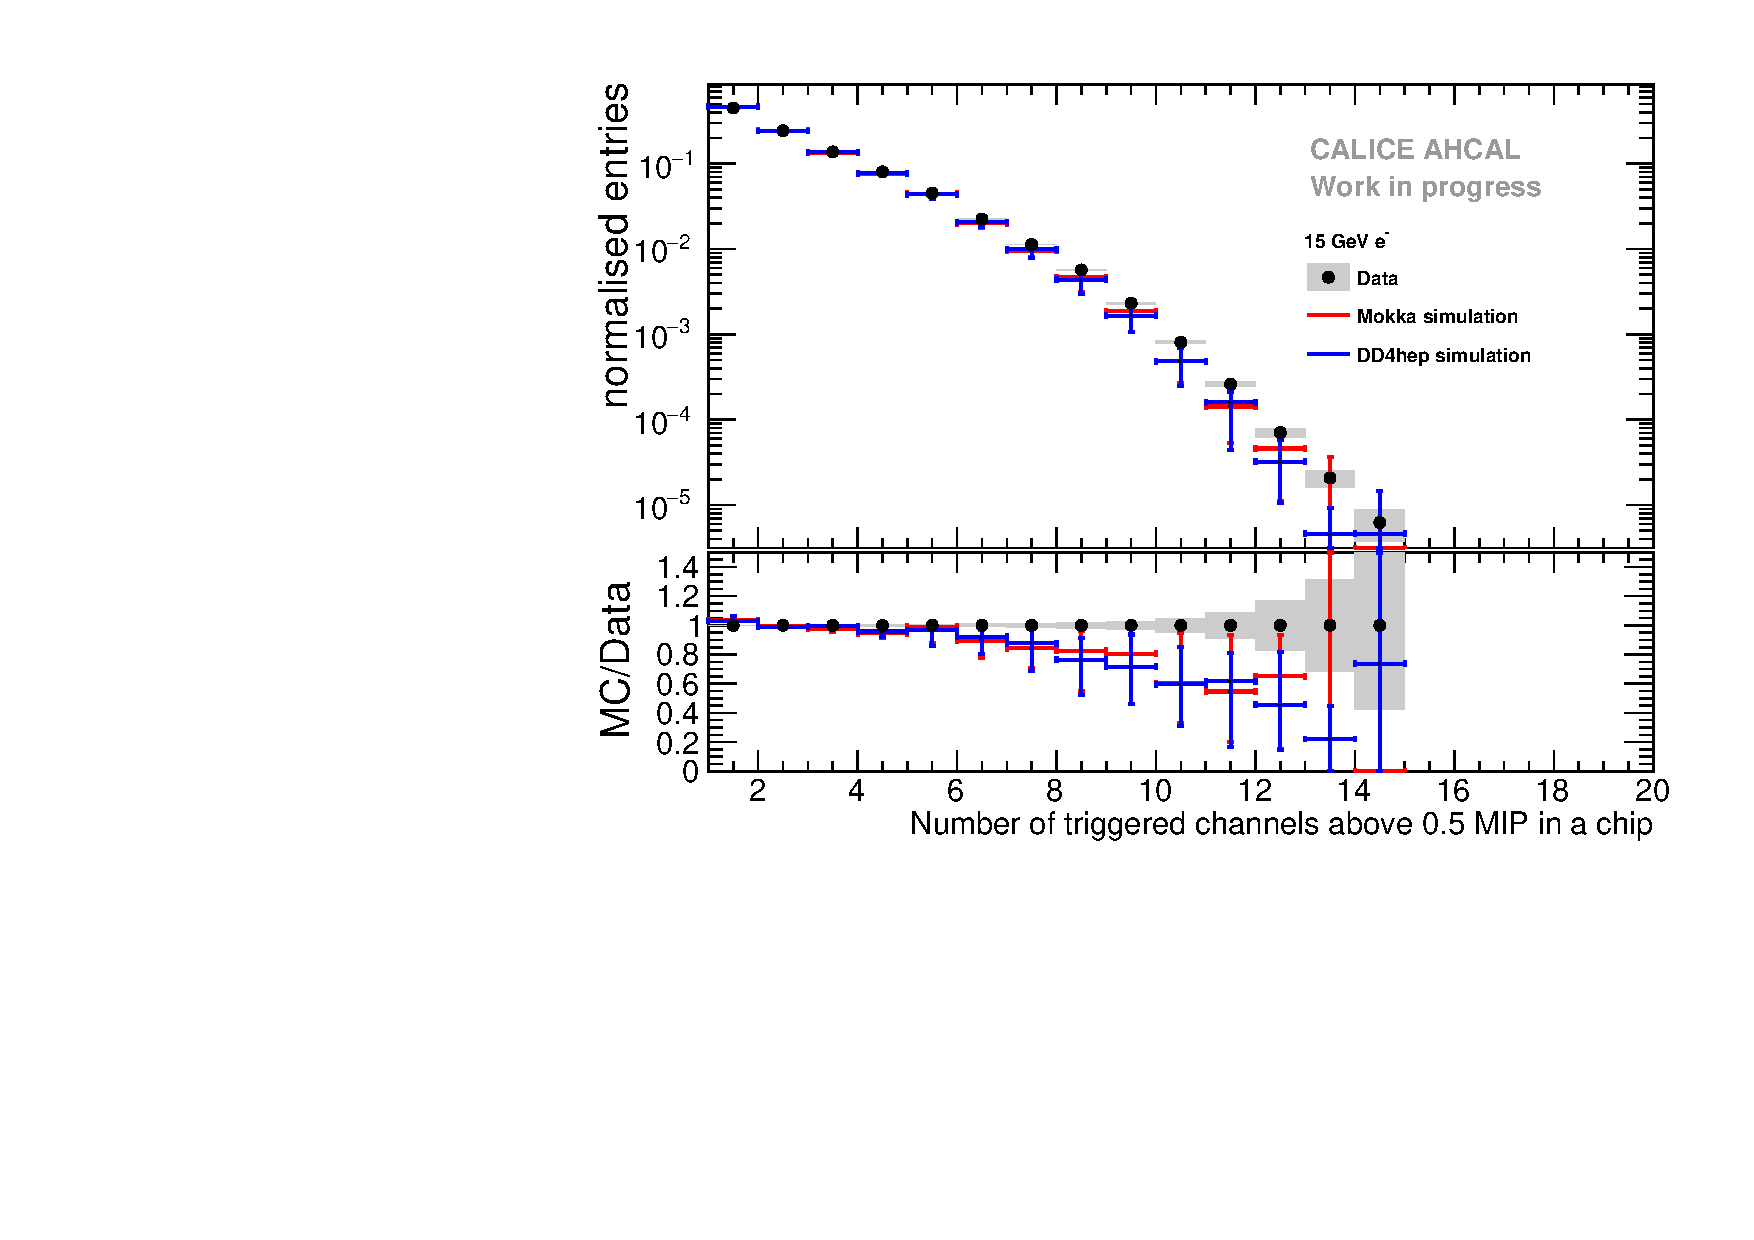
\includegraphics[width=1\textwidth]{chap5/fig_AHCAL_timing/Electrons/Comparison_SimData_Electrons_nHits_15GeV.pdf}
		\caption{15 GeV.}\label{fig:elec_sim_data_nHits_15GeV}
	\end{subfigure}
	\hfill
	\begin{subfigure}[t]{0.45\textwidth}
		\centering
		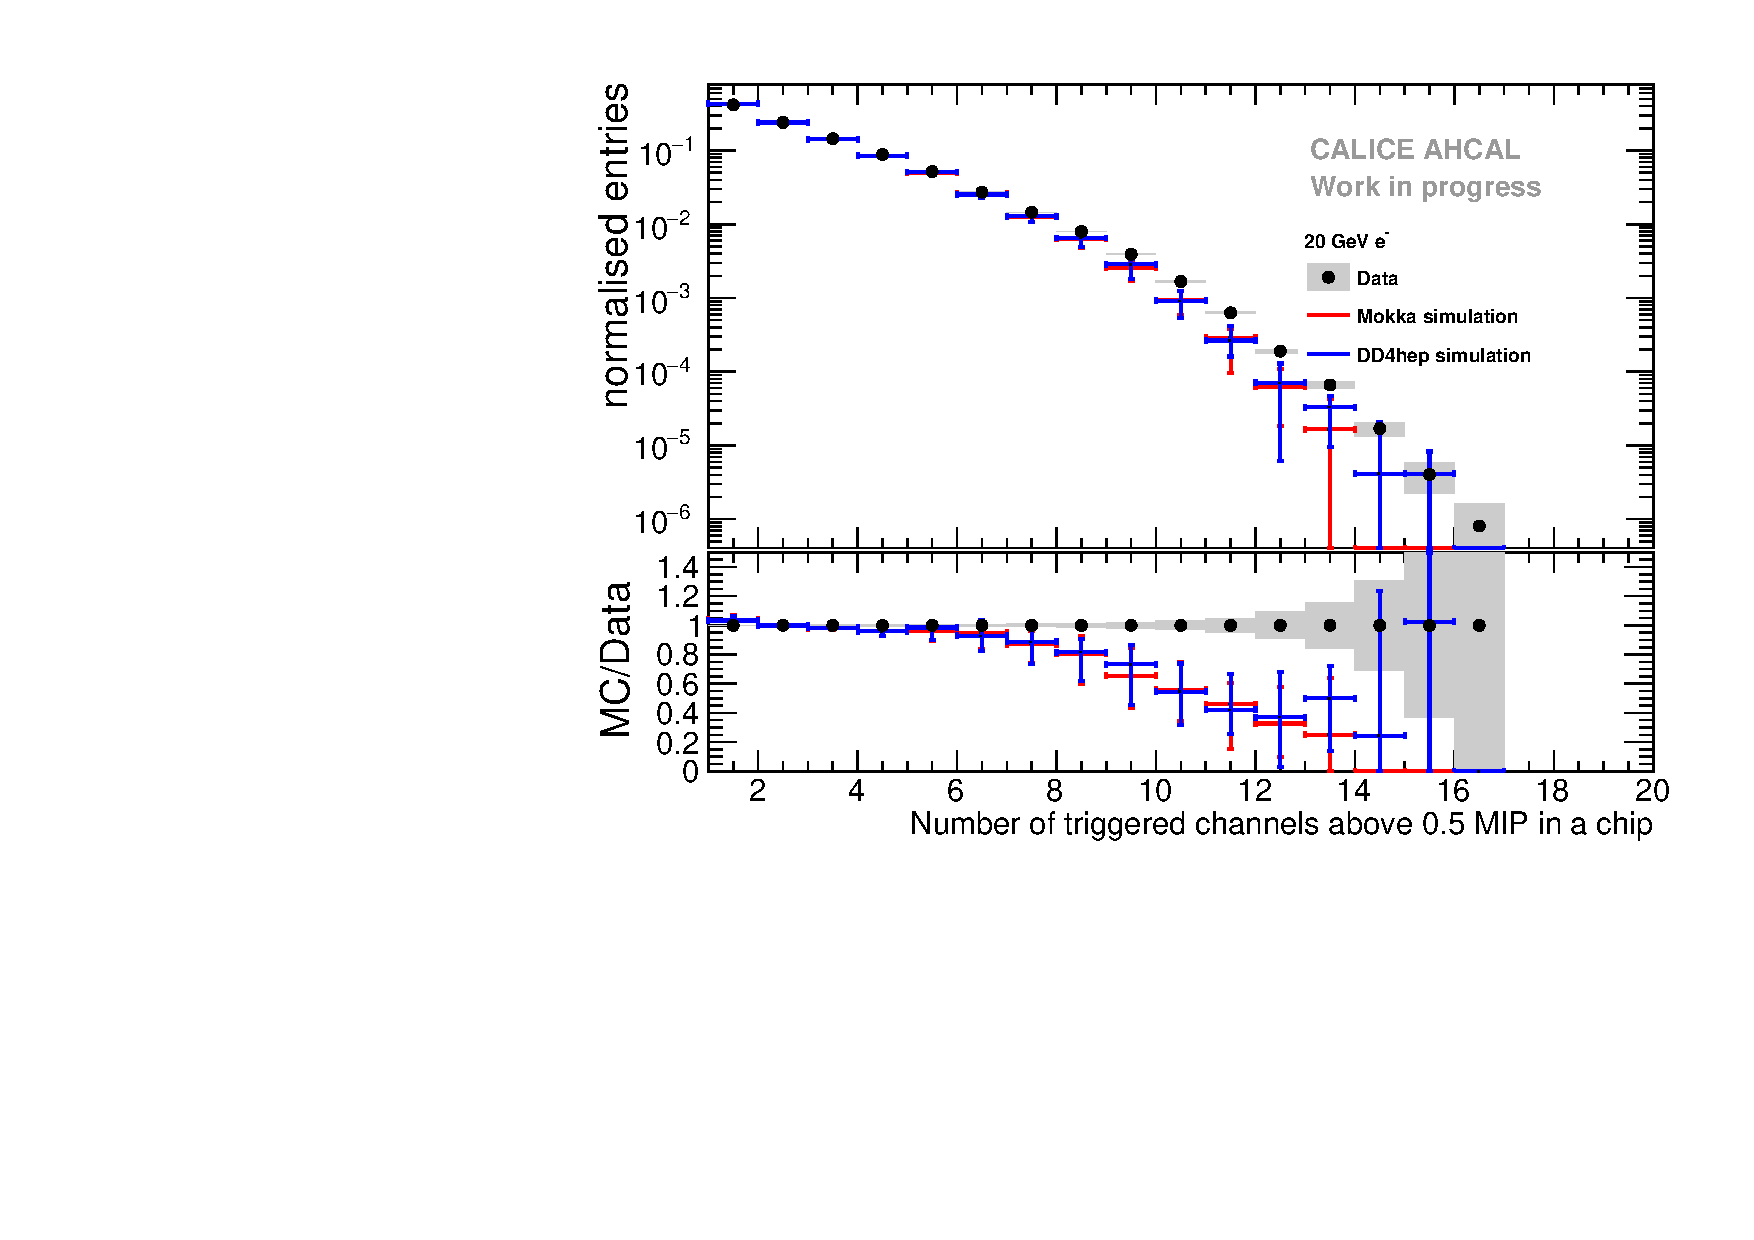
\includegraphics[width=1\textwidth]{chap5/fig_AHCAL_timing/Electrons/Comparison_SimData_Electrons_nHits_20GeV.pdf}
		\caption{20 GeV.}\label{fig:elec_sim_data_nHits_20GeV}
	\end{subfigure}
	\hfill
	\begin{subfigure}[t]{0.45\textwidth}
		\centering
		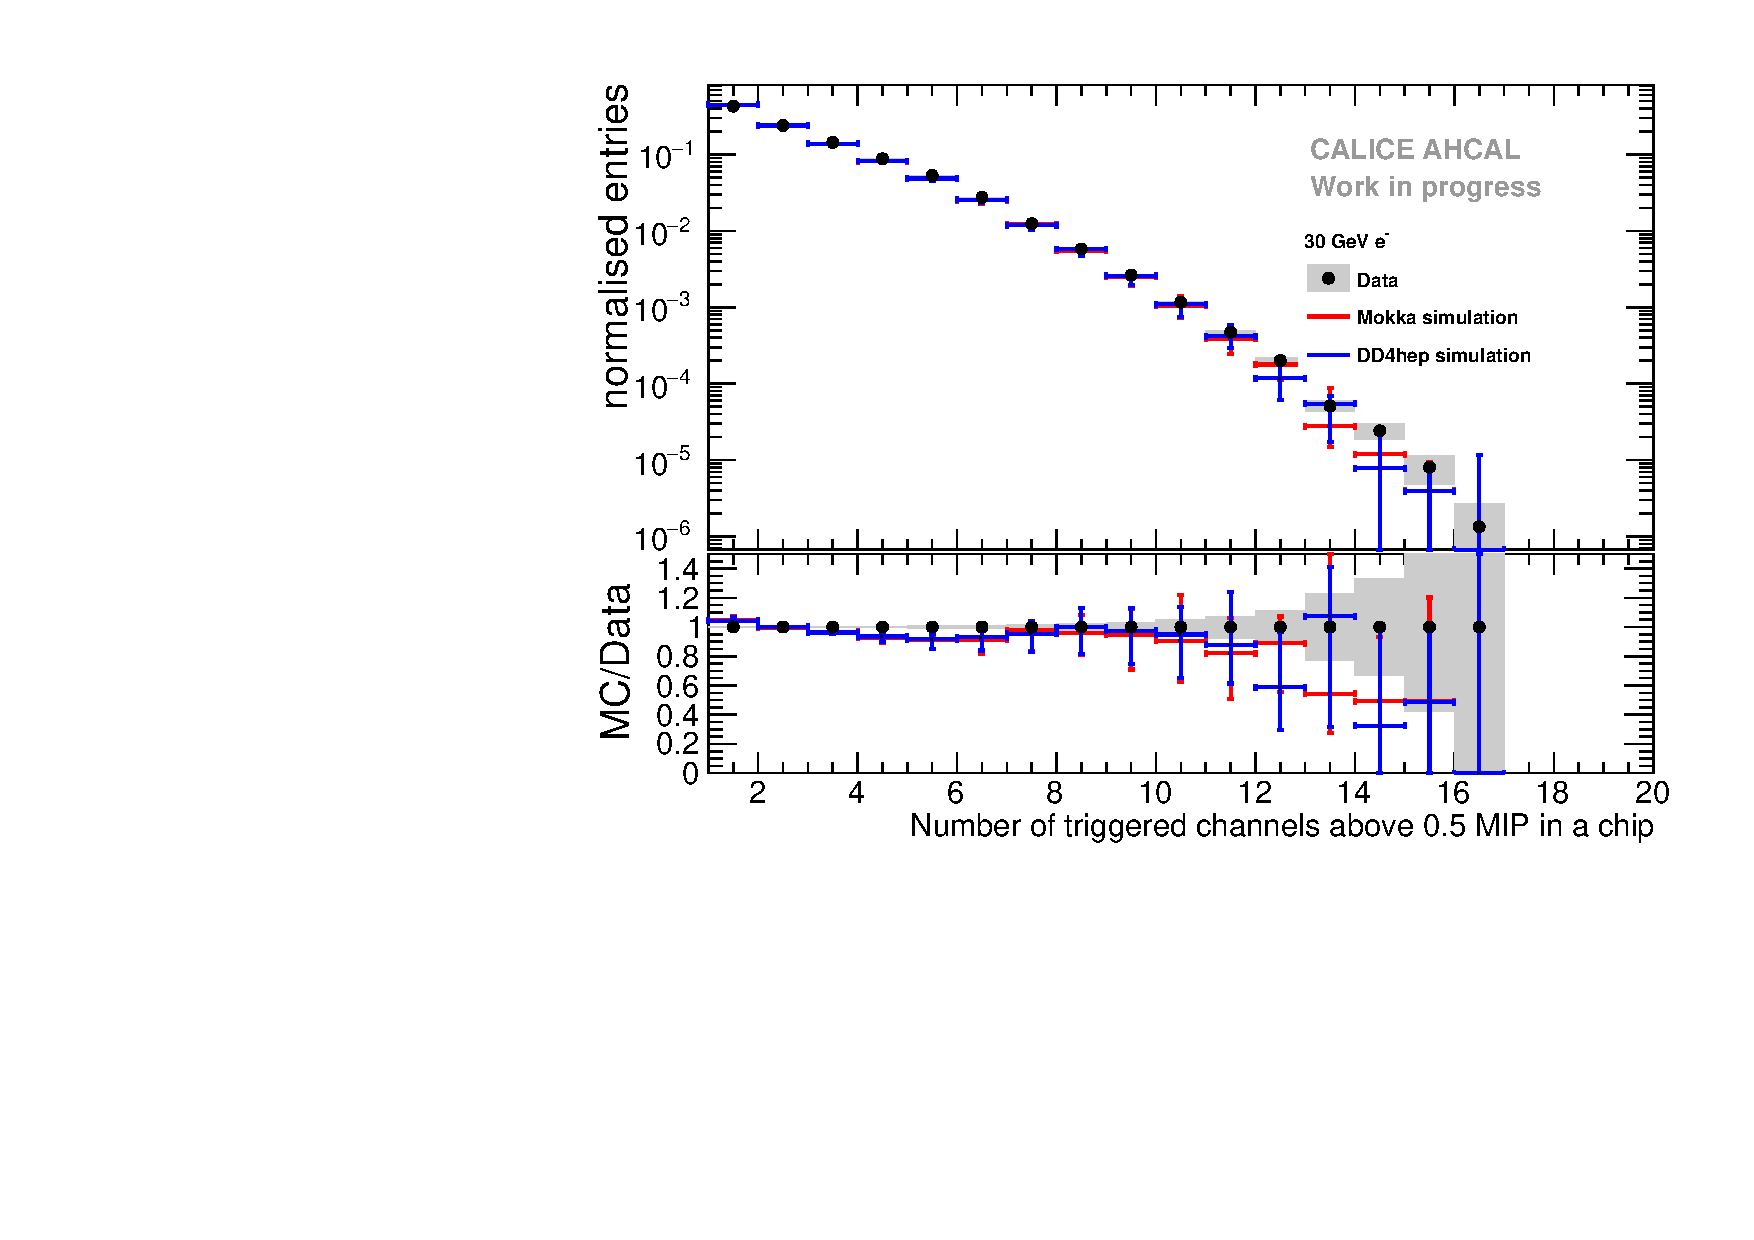
\includegraphics[width=1\textwidth]{chap5/fig_AHCAL_timing/Electrons/Comparison_SimData_Electrons_nHits_30GeV.pdf}
		\caption{30 GeV.}\label{fig:elec_sim_data_nHits_30GeV}
	\end{subfigure}
	\hfill
	\begin{subfigure}[t]{0.45\textwidth}
		\centering
		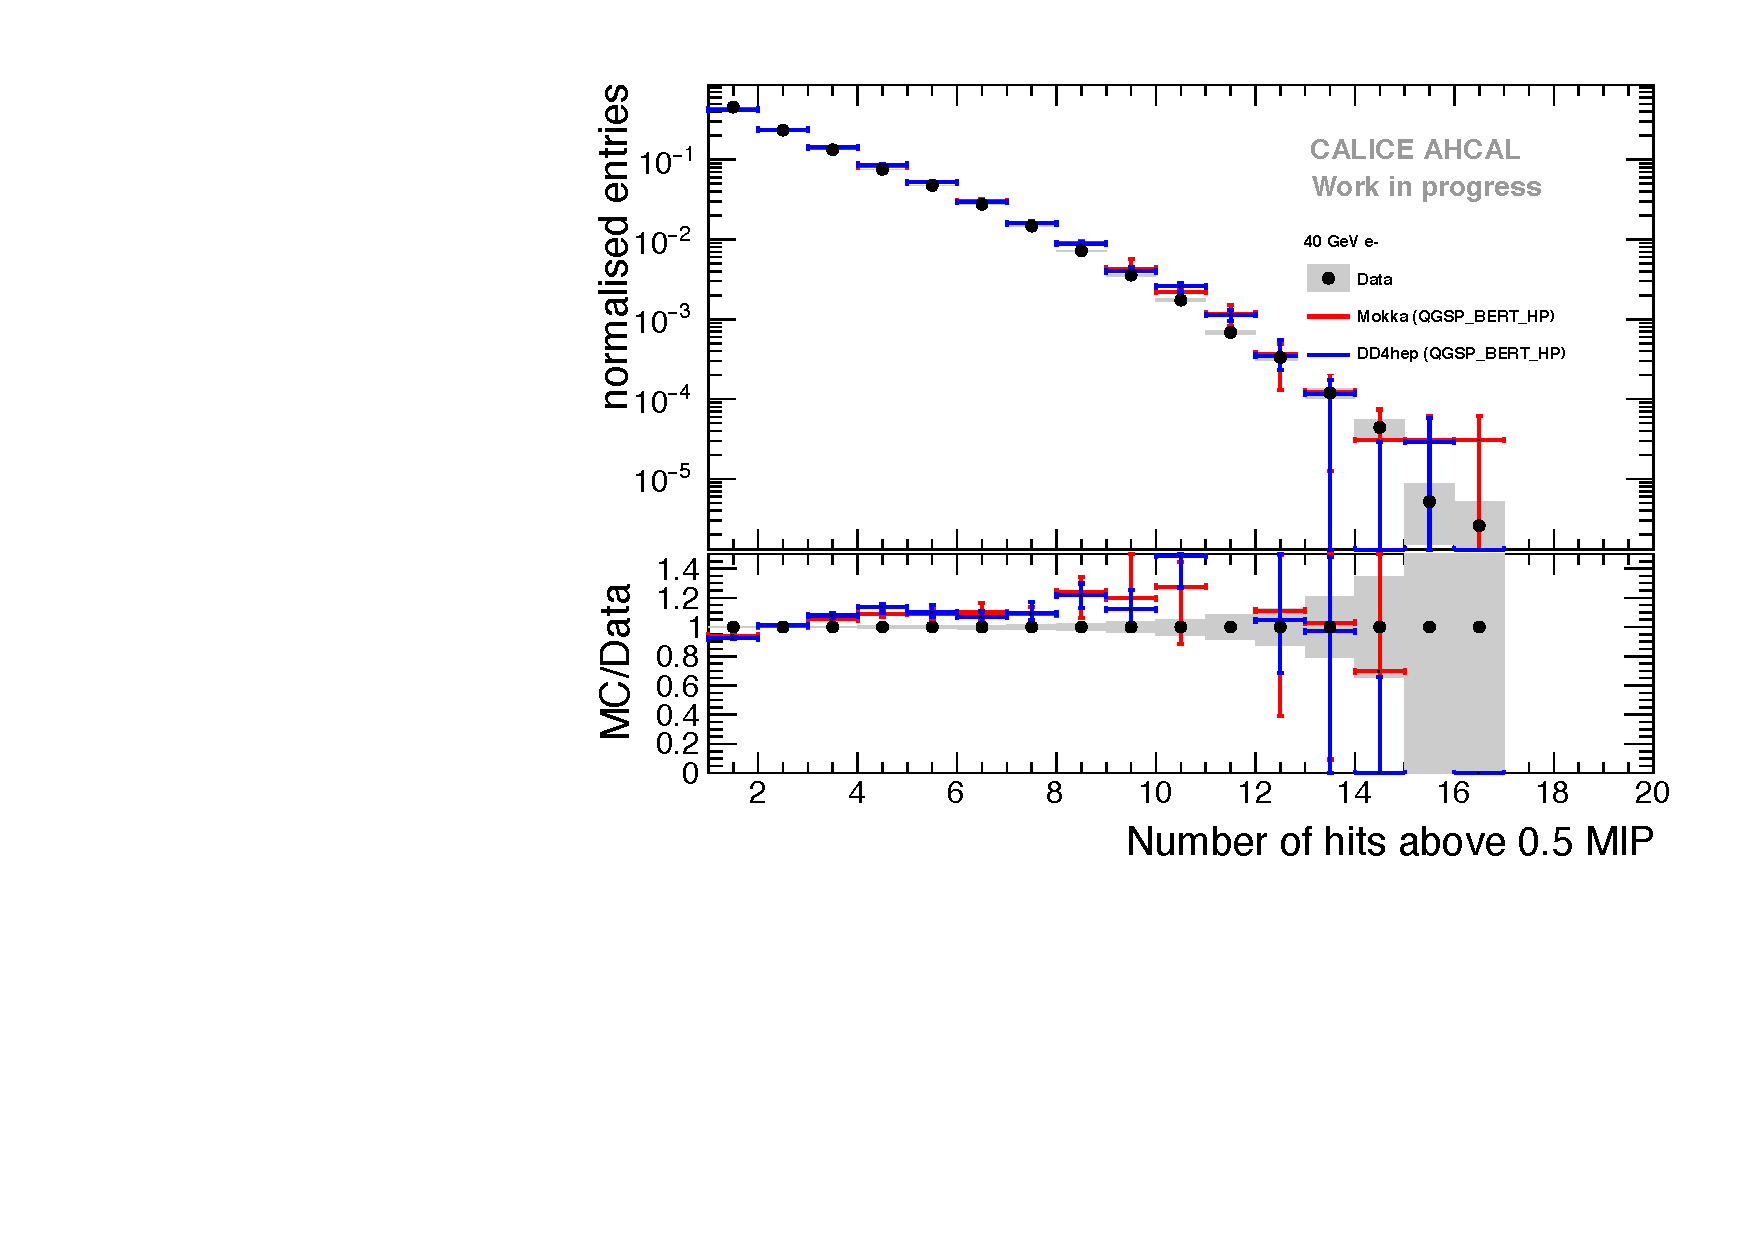
\includegraphics[width=1\textwidth]{chap5/fig_AHCAL_timing/Electrons/Comparison_SimData_Electrons_nHits_40GeV.pdf}
		\caption{40 GeV.}\label{fig:elec_sim_data_nHits_40GeV}
	\end{subfigure}
	\hfill
	\begin{subfigure}[t]{0.45\textwidth}
		\centering
		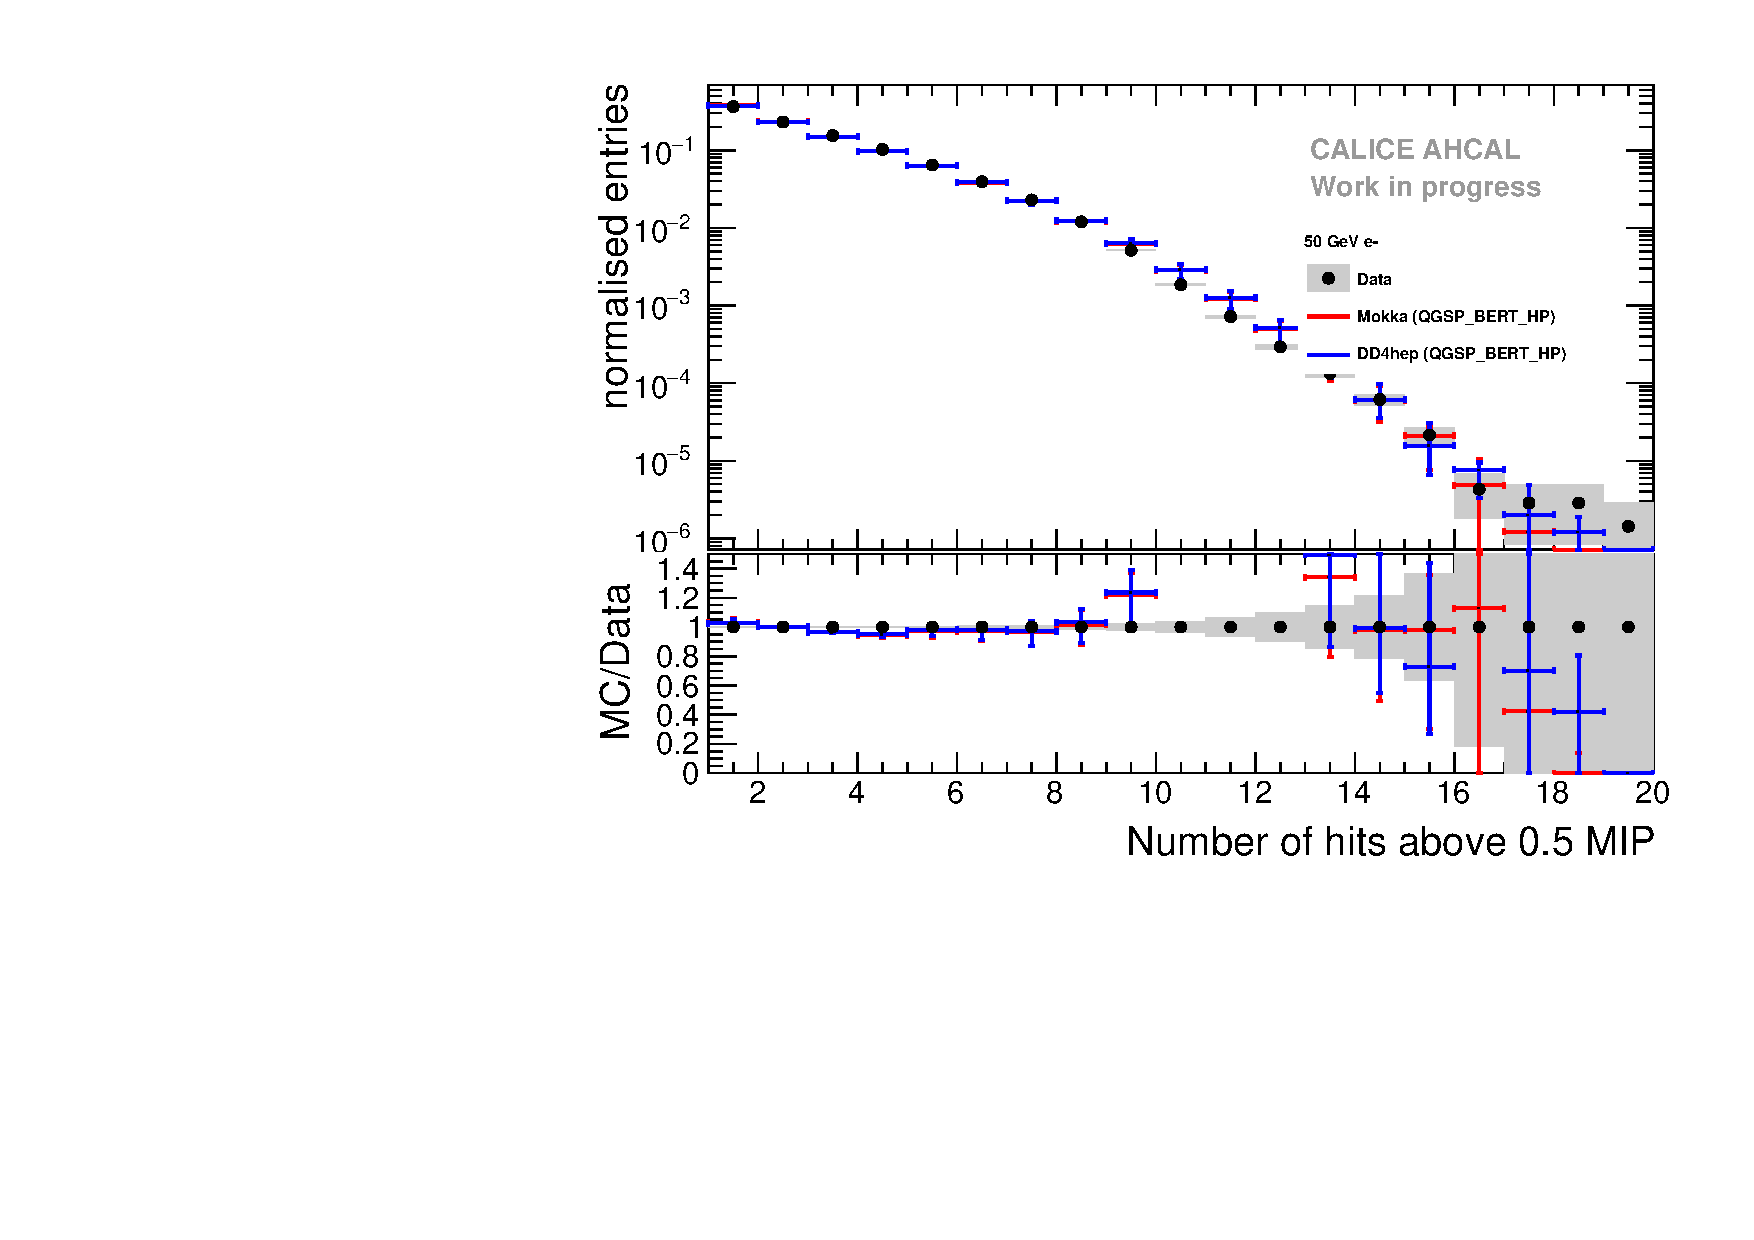
\includegraphics[width=1\textwidth]{chap5/fig_AHCAL_timing/Electrons/Comparison_SimData_Electrons_nHits_50GeV.pdf}
		\caption{50 GeV.}\label{fig:elec_sim_data_nHits_50GeV}
	\end{subfigure}
	\caption{Comparison between electron data and MC for all energies of the number of triggered channels per chip. The grey area represents the statistical error of the data. Error bars in simulation are obtained by varying the cross-talk parameter between 10\% and 18\%.}
	\label{fig:sim_data_elec_nHits}
\end{figure}

\newpage
\section{Results}

One of the main goal is to compared \geant simulation with different hadronic physics models to the recorded pion data. The table \ref{table:pion_runs} summarises the runs and datasets used.

\begin{table}[htb!]
	\centering
	\caption{Table with the statistic before and after selection used for the pion dataset.}
	\label{table:pion_runs}
	\resizebox{0.9\textwidth}{!}{%
	\begin{tabularx}{\textwidth}{>{\hsize=1.1\hsize}Xlllll}
		\hline
		Runs & Energy & Particle Type & Events (3 T0s) & Events (sel.) & $\frac{\text{N$_{sel.}$}}{\text{N$_{raw}$}}$ \\
		\hline
		24306-24317 \newline 24381-24397 & 10 GeV & $\pi^-$ & 425517 & 349012 & 82\% \\
		24578-24612 & 50 GeV & $\pi^-$ & 1183790 & 1007889 & 85.1\% \\
		24339-24342 & 70 GeV & $\pi^-$ & 142813 & 122376 & 85.7\% \\
		24223-24238 \newline 24273-24287 \newline 24331-24336 \newline 24358-24364 & 90 GeV & $\pi^-$ & 466927 & 395884 & 84.8\% \\
		\hline
	\end{tabularx}
	}
\end{table}


\section{Summary}
